\documentclass[report,paper=a4, fontsize=12pt, line_length=16cm, number_of_lines=33,dvipdfmx]{jlreq}
%\documentclass[pandoc,12pt]{bxjsarticle}

\usepackage{amsmath,amssymb}
\usepackage[bold,uplatex]{otf}
%% Fonts
\usepackage[T1]{fontenc}
\usepackage{tgtermes,tgheros,tgcursor}
\renewcommand{\bfdefault}{bx}
\usepackage[libertine]{newtxmath}
\usepackage{hyperref}
\usepackage{pxjahyper}

\usepackage{graphicx}
\graphicspath{{fig/}}

\usepackage{physics}
\usepackage{color}

\usepackage{tcolorbox}
\tcbuselibrary{breakable, skins, theorems}
%\usepackage{cleveref}

% font warningを出さないため
\DeclareFontShape{JY2}{hgt}{b}{n}{<->ssub*hgt/bx/n}{}
\DeclareFontShape{JY2}{hgt}{m}{it}{<->ssub*hgt/m/n}{}
\DeclareFontShape{JT2}{hgt}{b}{n}{<->ssub*hgt/bx/n}{}
\DeclareFontShape{JT2}{hgt}{m}{it}{<->ssub*hgt/m/n}{}

\newenvironment{myquote}{\begin{tcolorbox}[
  colback = blue!5, after = \noindent] }{\end{tcolorbox}}
\newenvironment{important}{\begin{tcolorbox}[
  colback = white,
  colframe = red!35,
  boxrule = 2mm,
  fonttitle = \bfseries,
  after = \noindent] }{\end{tcolorbox}}
\newenvironment{mycite}{\\ \qquad \textbullet\ }{\\}

\numberwithin{equation}{chapter}
%%%%%%%%%%%%%%%%%%%%%%%%%%%%%%%%%%%%%%%%%%%%%%%%%%%%%%%%%%%%%%%%%%%%%%
%                          often used macro
\newcommand{\del}{\partial}
\newcommand{\Cb}{\mathbb{C}}
\newcommand{\Zb}{\mathbb{Z}}
\newcommand{\CP}{\Cb \mathrm{P}}
\newcommand{\strong}[1]{{\sffamily \bfseries #1}}
\newcommand{\Sp}{S$'$}

\newcommand{\psib}{\overline{\psi}}
\newcommand{\phit}{\tilde{\phi}}
\newcommand{\dell}{\overleftarrow{\del}}
%\newcommand{\ad}{\mathrm{ad}}
\DeclareMathOperator{\ad}{\mathrm{ad}}
\newcommand{\xb}{\vvmathbb{x}}
\newcommand{\nb}{\vvmathbb{n}}
\newcommand{\eb}{\vvmathbb{e}}
\newcommand{\kb}{\vvmathbb{k}}
\newcommand{\jb}{\vvmathbb{j}}
\newcommand{\pbb}{\vvmathbb{p}}
\newcommand{\Ab}{\vvmathbb{A}}
\newcommand{\Bb}{\vvmathbb{B}}
\newcommand{\Lb}{\vvmathbb{L}}
\newcommand{\Sb}{\vvmathbb{S}}
\newcommand{\Jb}{\mathbb{J}}
\newcommand{\Eb}{\vvmathbb{E}}
\newcommand{\bnabla}{\raisebox{-0.2ex}{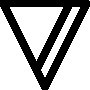
\includegraphics[width=0.65em]{bnabla.pdf}}}
\newcommand{\alphab}{\vmathbb{\alpha}}
\newcommand{\zerob}{\vmathbb{0}}


\newcommand{\uket}{\ket{\uparrow}}
\newcommand{\dket}{\ket{\downarrow}}
\newcommand{\ml}{m_{l}}

\newcommand{\Fii}{{}_1F_1}

\newcommand{\Lcal}{\mathcal{L}}
\newcommand{\Hcal}{\mathcal{H}}

\newcommand{\ao}[1]{\textcolor{blue}{#1}}
\newcommand{\aka}[1]{\textcolor{red}{#1}}

\newcommand{\dk}{\frac{d^3\kb}{(2\pi)^3}}






\newcommand{\phih}{\hat{\phi}}
\newcommand{\chih}{\hat{\chi}}
\newcommand{\pih}{\hat{\pi}}
\newcommand{\Hh}{\widehat{H}}
\newcommand{\Ah}{\widehat{A}}
\newcommand{\Bh}{\widehat{B}}
\newcommand{\ah}{\hat{a}}
\newcommand{\Nh}{\widehat{N}}
\newcommand{\Ph}{\widehat{P}}

\title{相対論的量子力学}
\author{山口 哲}
\date{\today}
\begin{document}

\maketitle
\tableofcontents
\subsubsection*{まえがき}
これは、大阪大学理学部物理学科の専門科目「相対論的量子力学」の授業のための資料です。2020年の新型コロナウイルスの流行対策としてのオンライン授業のために作成しました。授業に参加し、この資料の間違いを指摘してくれた2020年の受講生の方々に感謝します。

この資料の再配布等は自由に行っていただいて結構です。

\chapter{導入}
この講義のタイトルは「相対論的量子力学」です。文字通り量子力学を相対論的にしようという試みです。まず、相対論と量子力学について、どんなものだったか思い出しましょう。

ここでは相対論とは、特殊相対論のことです\footnote{実は、物理の研究者が「相対論」と言うと、多くの場合は一般相対論を指します。}。特殊相対論とはLorentz変換によって物理法則が不変になるという、理論の枠組みのことでした。
特に\strong{Lorentz変換は、時刻$t$と空間の位置$\xb$を混ぜる変換}ですので、理論の記述の中には、時間と空間は同等に入っていることが望ましいです
\footnote{実際には、物理量がLorentz変換の対称性を持てばよいので、理論の記述ではLorentz対称性は明らかではないかもしれません。
現代的な物理では、「物理量」と「理論の記述」を区別することが重要です。}。

もう一方の量子力学は、Schrödinger方程式で記述されるような、波動関数を考えるものでした。ポテンシャル$V(\xb)$中の1粒子の場合だと波動関数を$\psi(t,\xb)$として、
\begin{align}
  i\hbar\pdv{t} \psi=\qty(
    -\frac{\hbar^2}{2m}\bnabla^2+V(\xb)
  )\psi\label{Schroedingereq}
\end{align}
というふうになります。ここでは、時刻$t$については1階微分ですが、位置$\xb$については2階微分になっているので、これらは同等に扱われていません。
1粒子の場合では1階か2階かという程度の問題ですが、多粒子になるともっと問題が大きくなります。
例えば2粒子の場合だと時刻は1つしかないのに空間の位置は2つあります。

この後、講義で説明するように量子力学を相対論的に書き換えようとすると、困難に直面します。
その一部は\strong{Dirac方程式}を考えることで克服できます。このDirac方程式は1つの電子をそれなりに良く記述します。
これは、大変素晴らしいもので、例えば非相対論的量子力学では「手で」入れていたスピンという角運動量が、Dirac方程式の立場からは自然に導入されます。
この講義の大部分は、このDirac方程式による1つの電子の記述についてです。

Dirac方程式による1つの電子の記述は素晴らしいものですが、まだ困難は残っています。Diracはそれを克服するために「Diracの海」という概念を導入しました。
これについては、後で詳しく説明します。
このDiracの海の概念も反粒子を予言するという素晴らしい成果を残しましたが、同時に\strong{1つの電子だけを考える理論は不完全で、必ず多粒子を考えなければならない}ということも明らかにします。

結局、正しく相対論的に量子力学を記述できる理論は、次の2つの条件を満たさなければなりません。
\begin{itemize}
  \item 任意個の粒子をいっぺんに取り扱うことができる。
  \item 粒子の「個数」、「種類」が時間発展で変わりうる。
\end{itemize}
こういう条件を満たす理論が\strong{場の理論}です。この場の理論の初歩的な導入をこの講義の後半で行います。

ここで強調したいのは、量子力学を相対論的に書き換えたいという「ちょっとした」動機から始まって、様々な困難に出会い克服していくうちに、場の理論という非常に大掛かりな理論に\strong{必然的に}行かなければならないことが分かったという点です。
物理の発展の歴史の中でも、もっともドラマチックな展開の1つだと思います。
理論的な考察が大きな役割を果たしたという点も、理論物理をやっている者としては興味深い点です。

参考文献を紹介します。1つめは昔からあるこの分野の名著で
\begin{mycite}
  西島和彦「相対論的量子力学」
\end{mycite}
です。Dirac方程式の取り扱いについて非常に詳しく書かれています。場の理論に行かない範囲内での電磁気の相互作用についても書かれています。もう1つは比較的新しい本で
\begin{mycite}
  坂本眞人「場の量子論―不変性と自由場を中心にして―」
\end{mycite}
です。非常に読みやすい本です。自由場についても比較的詳しく書かれています。

\chapter{準備}
ここでは、量子力学を相対論的に書き換えるための準備をします。まず、自然単位系という便利な単位系を導入します。そして、特殊相対論と量子力学の中から必要なことを復習します。

\section{自然単位系}
この分野では、複雑な式がたくさん出てきます。
その式の見た目の複雑さを少しでも軽減するために単位をうまくとって基本的な物理定数を$1$にすることを考えます。2つだけ注意をしておきます。
\begin{itemize}
  \item このような単位系を選ぶのは、単に式の見た目を簡単にするという便利のためであって物理の本質とは全く関係ありません。SI単位系を用いて全く同じように物理を記述することができます。
  \item 物理定数をあらわに書いたほうが便利なこともあります。このようなときには、次元解析により物理定数を式の中に復活させることは、いつでもできます。復活させる練習をしておくことは重要です。
\end{itemize}

まず、我々は特殊相対論を取り扱います。特殊相対論では真空中の光速$c$は非常に基本的な定数で、そこらじゅうに現れます。ですので時間の単位をとりかえて$c=1$となる単位系をとれば式が簡単になると期待できます。例えば、長さを[m](メートル)で測ったとして、時間も[m]で測ることになります。時間1 mは真空中を光が1 m進むのにかかる時間です。

また、我々は量子力学を取り扱います。量子力学ではプランク定数を$2\pi$で割ったもの$\hbar$は非常に基本的な定数で、たくさん現れます。なのでエネルギーの単位をとりかえて$\hbar=1$になるようにすると便利です。例えば先程のように長さと時間の単位を[m]にしたとします。角振動数は角度を時間で割ったものですから、その単位は[m${}^{-1}$]になります。なのでエネルギーの単位を[m${}^{-1}$]とすると$\hbar=1$にすることができます。この場合エネルギー1 m${}^{-1}$は、角振動数1 m${}^{-1}$の光子1個が持つエネルギーになります。

このように$c=1,\hbar=1$とした単位系を\strong{自然単位系}といいます\footnote{この講義では関係ないですが、$c=1, \hbar=1$に加えてボルツマン定数$k_B=1$となるように温度の単位も選んだものを自然単位系と呼ぶことも多いです。}。自然単位系では、まだ1つだけ単位を自由に選ぶことができます。例えば上では、長さの単位[m]を選びました。素粒子論でよく使うのはエネルギーの単位を1つ選ぶことです。例えばエネルギーの単位を[GeV](ギガ電子ボルト)と選んだとすると、長さや時間は[GeV${}^{-1}$]で表すことになります。

ちなみに、これに関して覚えておくと便利な数字があります。
\begin{align}
  \hbar c = 0.20 \mathrm{\ GeV\cdot fm}\label{fmGeV}
\end{align}
というものです。ここで1 fm $=10^{-15}$mです。1 fmはだいたい原子核の大きさくらいのスケールです。\eqref{fmGeV}の意味するところは、自然単位系では$1\ \mathrm{ fm}=\frac{1}{0.20}\ \mathrm{GeV}^{-1}$ということです。

\section{特殊相対論のテンソル}
特殊相対論のテンソルの記号の使い方等は、付録\ref{app:tensor}にまとめています。ひととおり復習しておいてください。1つだけ注意することは、$\eta_{\mu\nu}$の符号についてです。今回の記号の使い方では、時空の計量は
\begin{align}
  \dd{s}^2=\eta_{\mu\nu}\dd{x}^{\mu}\dd{x}^{\nu}=+(\dd{x}^0)^2
  -(\dd{x}^1)^2
  -(\dd{x}^2)^2
  -(\dd{x}^3)^2\label{metric}
\end{align}
となります。私の電磁気学2の講義を受けた人は、そのときと符号が逆であることに注意してください。人、教科書、時と場合によって、この符号はどちらを使っているかが違います。今後教科書、論文などを読むときは注意してください。

\section{Maxwell理論}
ここでは、Maxwell理論のテンソルの記号を用いた表記について復習します。テンソルの記号を用いて書くと、シンプルになるというのみならず、Poincar\'e不変性が明らかになります。ここでやるのはあくまで復習です。もし、この節でやることを今までやったことがなければ、ちゃんとした教科書で勉強してください。

みなさんが、1年生のときから習ってきたMaxwell方程式は次のようになっていたと思います。
\begin{align}
  &\bnabla \times \Eb + \pdv{t} \Bb = \zerob ,
  &&\bnabla \cdot \Bb =0,\\
  &\bnabla\cdot \Eb = \frac{1}{\epsilon_0}\rho,\quad
  &&\bnabla \times \Bb -\epsilon_0\mu_0 \pdv{t}\Eb =\mu_0 \jb.
\end{align}
ここで、光速$c$は、$c=\frac{1}{\sqrt{\epsilon_0\mu_0}}$と表すことができました。今、自然単位系をとっているので$c=1$であり、したがって$\epsilon_0 \mu_0=1$ となります。この関係を使って$\epsilon_0$を消すと
\begin{align}
  &\bnabla \times \Eb + \pdv{t} \Bb = \zerob ,
  &&\bnabla \cdot \Bb =0, \label{Bianchi}\\
  &\bnabla\cdot \Eb = \mu_0 \rho,\quad
  &&\bnabla \times \Bb - \pdv{t}\Eb =\mu_0 \jb\label{Maxwelleq}
\end{align}
というふうに書けます。さらに電荷の単位を調整して$\mu_0=1$となるようにすることもできますが、ここでは必要ないのでやりません。\footnote{電荷の単位を決めるのに$\mu_0=1$にするのが便利なこともありますが、$\mu_0$は残したままで電子の電荷を$-1$にするのが便利なこともあります。}

これを相対論的に書き換えていきます。何も言わなければ3次元ベクトルの成分は上付きで書くことにします。例えば$\Eb=(E^1,E^2,E^3)$です。

天下り的ですが、次のように$\Eb$と$\Bb$をまとめて反対称テンソル$F^{\mu\nu}$にします。
\begin{align}
  F^{\mu\nu}=\mqty(
    0 & -E^1 & -E^2 & -E^3\\
    E^1 & 0 & -B^3 & B^2 \\
    E^2 & B^3 & 0 & -B^1 \\
    E^3 & -B^2 & B^1 & 0
  ).\label{fieldstrength}
\end{align}
この書き方の意味は$F^{\mu\nu}$を4行4列の行列の$\mu\nu$成分とみなして、その行列を書いたものです。例えば$F^{10}=E^1$になります。$F^{\mu\nu}=-F^{\nu\mu}$であることに注意してください。

\eqref{fieldstrength}式の$F^{\mu\nu}$を用いるとMaxwell方程式の\eqref{Bianchi}式と\eqref{Maxwelleq}式はそれぞれ
\begin{important}
  \begin{align}
    \del_{[\mu}F_{\nu\rho]} =0,\label{Bianchi2}\\
    \del_{\mu}F^{\mu\nu}=\mu_0j^{\nu}\label{Maxwelleq2}
  \end{align}    
\end{important}
と書けます。ただし4元ベクトル$j^{\mu}$の$0$成分は$j^0=\rho$としました。また、\eqref{Bianchi2}では反対称化の記号$[]$を用いました。定義は
$T_{\mu\nu\rho}$に対して
\begin{align}
  T_{[\mu\nu\rho]}:=\frac{1}{3!}(T_{\mu\nu\rho}+T_{\nu\rho\mu}+T_{\rho\mu\nu}-T_{\nu\mu\rho}-T_{\mu\rho\nu}-T_{\rho\nu\mu})
\end{align}
です。もっと一般の場合には付録の\eqref{antisymmetrization}式を参照してください。今の場合には\eqref{Bianchi2}は
\begin{align}
  \del_{\mu}F_{\nu\rho}+\del_{\nu}F_{\rho\mu}+\del_{\rho}F_{\mu\nu}=0\label{Bianchi3}
\end{align}
と等価です。実際\eqref{Bianchi2}(あるいは\eqref{Bianchi3})と\eqref{Maxwelleq2}がそれぞれ\eqref{Bianchi}式と\eqref{Maxwelleq}式と等価であることは次のように確かめられます。
\begin{itemize}
  \item \eqref{Bianchi2}式あるいは\eqref{Bianchi3}式で$(\mu,\nu,\rho)=(0,i,j),\ i,j=1,2,3$としたものが、\eqref{Bianchi}の左の式になります。
  \item \eqref{Bianchi2}式あるいは\eqref{Bianchi3}式で$(\mu,\nu,\rho)=(1,2,3)$としたものが\eqref{Bianchi}の右の式になります。
  \item \eqref{Maxwelleq2}式で$\nu=0$としたものが\eqref{Maxwelleq}の左の式になります。  
  \item \eqref{Maxwelleq2}式で$\nu=i,\ i=1,2,3$としたものが\eqref{Maxwelleq}の右の式になります。
\end{itemize}
実際に手を動かして確かめてみてください。

さて、\eqref{Bianchi2}の式は「解く」ことができて、あるベクトル場$A_{\mu}$を用いて
\begin{important}
  \begin{align}
    F_{\mu\nu}=\del_{\mu}A_{\nu}-\del_{\nu}A_{\mu}\label{gaugefield}
  \end{align}    
\end{important}
と書くことができます。この$A_{\mu}$は電磁気の授業でならった電磁ポテンシャル$\phi,\Ab$と同じです。実際
\begin{align}
  \phi=A^{0},\quad \Ab=(A^1,A^2,A^3)
\end{align}
となっています。電磁場$\Eb,\Bb$が
\begin{align}
  \Eb=-\pdv{t}\Ab-\bnabla \phi,\quad \Bb=\bnabla \times \Ab
\end{align}
と書けるのでした。さらに、同じ$F_{\mu\nu}$を与える$A_{\mu}$は一意的でなく、任意の関数$\alpha$を用いて\strong{ゲージ変換}
\begin{align}
  A_{\mu} \to \tilde{A}_{\mu}=A_{\mu}+\del_{\mu}\alpha 
\end{align}
としても同じ$F_{\mu\nu}$を与えます。このゲージ変換で理論が不変であることを\strong{ゲージ対称性}といいます。ゲージ対称性は素粒子論で非常に重要な概念です。

\section{相対論的な自由粒子の古典力学}
さて、相対論的な粒子の運動について復習しましょう。ここでは解析力学の枠組みで見ていきます。まずは自由粒子からです。粒子が時空に描く線を\strong{世界線}と呼びます。自由粒子の作用は世界線の長さに比例します。これは、質量を$m$として
\begin{important}
  \begin{align}
    S=-m\int \dd{s}\label{actionfree}
  \end{align}    
\end{important}
と書けます。世界線をパラメータ表示するためのパラメータを$\lambda$とし、式\eqref{metric}の両辺を$d\lambda$で割って
\begin{align}
  \qty(\dv{s}{\lambda})^2=\eta_{\mu\nu}\dv{x^{\mu}}{\lambda}\dv{x^{\nu}}{\lambda}
\end{align}
となるので、\eqref{actionfree}の作用は
\begin{align}
  S=-m\int \dd{s}
  =-m\int \dd{\lambda}\dv{s}{\lambda}
  =-m\int \dd{\lambda}\sqrt{\eta_{\mu\nu}\dv{x^{\mu}}{\lambda}\dv{x^{\nu}}{\lambda}}
\end{align}
と書くことができます。ここで気づくことは、$\lambda$はちゃんとパラメータ付けできるようなものである限り何でもよいということです。別の言い方をすると、再パラメータ付け$\lambda\to \lambda'=\lambda'(\lambda)$の対称性があるということです\footnote{再パラメータ付けの対称性は広い意味でのゲージ対称性です。}。

再パラメータ付けの対称性を利用して$\lambda=t$という条件を付けることにします。このような操作を一般に\strong{ゲージを選ぶ}あるいは\strong{ゲージ固定}といいます。特に今の$\lambda=t$の条件を課すゲージ固定は\strong{静的ゲージ}と呼びます。こうすると、作用は
\begin{align}
  S=\int \dd{t} L,\quad L=-m\sqrt{1-\dot{\xb}^2}\label{staticgauge}
\end{align}
となります。$\dot{\xb}$は速度です。この表式では、明白なLorentz不変性は失われてしまっています。これは、静的ゲージという時間$t$を特別扱いしたゲージをとったためです。しかし、理論からLorentz不変性が失われたわけではないことに注意してください。

さて、\eqref{staticgauge}の作用を解析力学で習ったように取り扱うことにしましょう。このLagrangianには、$\dot{\xb}$は現れますが$\xb$そのものは現れない、つまり$\xb$は循環座標になっています。この場合、$\xb$を並進する対称性があり、$\xb$の正準運動量が保存します。これを求めてみましょう。$i=1,2,3$として定義にしたがって計算すると
\begin{align}
  p^i=\pdv{L}{\dot{x}^i}=\frac{m\dot{x}^i}{\sqrt{1-\dot{\xb}^2}}
\end{align}
となります。つまり、3次元ベクトルの記法を用いると
\begin{align}
  \pbb=\frac{m\dot{\xb}}{\sqrt{1-\dot{\xb}^2}}
\end{align}
となります。

一方、Lagrangianは時間$t$に陽によっていないので時間並進の対称性もあります。時間並進対称性の保存量であるエネルギーは
\begin{align}
  E=\pbb\cdot \dot{\xb}-L=\frac{m}{\sqrt{1-\dot{\xb}^2}}
\end{align}
となります。時間方向並進と空間方向並進は合わせて4元ベクトルを組んでいるので、その保存量である$E$と$\pbb$も合わせて4元ベクトルになっていると期待できます。実際$p^0=E$としたとき、$p^{\mu}$が4元反変ベクトルになっています。例えば$p^2$を計算してみると
\begin{align}
  p^2=\eta_{\mu\nu}p^{\mu}p^{\nu}=E^2-\pbb^2
=\frac{m^2}{1-\dot{\xb}^2}-\frac{m^2\dot{\xb}^2}{1-\dot{\xb}^2}
\end{align}
となり、
\begin{important}
  \begin{align}
    p^2=m^2\label{p2}
  \end{align}  
\end{important}
というスカラーを得ます。式\eqref{p2}になると、また明白なLorentz不変性があります。

\section{電磁場背景中の粒子}
\label{classicalelemagbackground}
ここでは、電磁場背景中の電荷を持った粒子を考えることにしましょう。運動方程式には、電場や磁場あるいはそれをまとめた$F_{\mu\nu}$しか出てこないですが、作用を書くためには電磁ポテンシャル$(\phi, \Ab)$あるいはそれをまとめた\eqref{gaugefield}式の$A_{\mu}$が必要になります。
% \begin{align}
%   \phi=A^0,\quad \Ab=\mqty(A^1 \\ A^2 \\ A^3)
% \end{align}
% としたとき$A^{\mu}$は4元反変ベクトルになっています。

少々天下り的ですが、電荷$q$をもつ粒子の作用は
\begin{align}
  S=-m\int \dd{s}-q\int A_{\mu}\dd{x}^{\mu}
\end{align}
となります。これが、Lorentz対称性およびゲージ対称性を保っていることは確かめることができます。静的ゲージをとると
\begin{align}
  S=\int \dd{t}L,\quad
  L=-m\sqrt{1-\dot{\xb}^2}-qA_{0}-qA_{i}\dot{x}^{i}
  \label{emstaticgauge}
\end{align}
となります。

ここで、前と同じように正準運動量を求めると
\begin{align}
  p^{i}=\pdv{L}{\dot{x}^i}
  =\frac{m\dot{x}^i}{\sqrt{1-\dot{\xb}^2}}-qA_{i}
  =\frac{m\dot{x}^i}{\sqrt{1-\dot{\xb}^2}}+qA^{i}
\end{align}
となります。ここで$A_i=-A^i$であることに注意してください。正準運動量はゲージ場によっているのがちょっと不思議です\footnote{これはゲージ変換をすると変化してしまいますから、物理量ではありません。}。そこで粒子の運動だけによる「運動学的運動量」$K^i$も定義しておきます。
\begin{align}
  K^i:=p^i-qA^{i}=\frac{m\dot{x}^i}{\sqrt{1-\dot{\xb}^2}}.
\end{align}
これは、電磁場がないときの運動量と同じです。同様にエネルギーを求めると
\begin{align}
  E=p^i\dot{x}^i-L
  =p^i\dot{x}^i+m\sqrt{1-\dot{\xb}^2}+qA_{0}+qA_{i}\dot{x}^{i}
  =K^i\dot{x}^i+m\sqrt{1-\dot{\xb}^2}+qA_{0}
  =\frac{m}{\sqrt{1-\dot{\xb}^2}}+qA_{0}
\end{align}
となります。$A_0=A^0$であることに注意して$K^0:=E-qA^0$は
\begin{align}
  K^0:=E-qA^0=\frac{m}{\sqrt{1-\dot{\xb}^2}}\label{kinematicalenergy}
\end{align}
となって、電磁場がないときのエネルギーと同じになります。$K^{\mu}=p^{\mu}-qA^{\mu}$ですので、$K^{\mu}$はまた4元反変ベクトルになります。これは、電磁場が無いときの4元運動量なので
\begin{align}
  K^2=(p-qA)^2=m^2
\end{align}
を満たします。

まとめると電磁場が入ったときの運動量の関係は
\begin{important}
  電磁場$A_{\mu}$が入る\ $\Rightarrow$\ $p_{\mu}\to p_{\mu}-qA_{\mu}$の置き換え
\end{important}
をやればよいことになります。実はこれには深い意味があり、ゲージ対称性から説明することができます。それは、この講義の後の方で出てきます。

\section{量子力学における確率の保存}
量子力学における重要な原理の1つは確率解釈です。通常の1粒子の量子力学で、この確率解釈がどのように成り立っていたかを思い出してみましょう。

1粒子のSchrödinger方程式\eqref{Schroedingereq}を考えましょう。自然単位系でもう一度書いてみると
\begin{align}
  i\dv{t} \psi=\qty(-\frac{1}{2m}\bnabla^2+V(\xb))\psi
\end{align}
でした。このとき位置$\xb$にいる確率密度は規格化の定数を除いて
\begin{align}
  \rho(t,\xb)=\psi^{*}\psi
\end{align}
でした。まず、これは確率密度であるための必要条件$\rho\ge 0$を満たします。規格化の定数は
\begin{align}
  Z(t)=\int \dd[3]{\xb}\rho(t,\xb) 
\end{align}
とします。この$Z(t)$が実は時間によらないというのは自明なことではありません。もし、この$Z(t)$が時間によらなければ、$\psi \to \psi'=\psi/\sqrt{Z}$というふうに規格化しなおすことにより、全確率を$1$にすることができます。

では、$Z(t)$が時間によらないことは、どのようにして証明できるでしょうか。ここで、電磁気で習った電荷の保存則がどのように示せるかを思い出してみましょう。電荷密度$\rho(t,\xb)$に対して、電流密度$\jb(t,\xb)$が存在して、Maxwell方程式から
\begin{important}
  \begin{align}
    \pdv{t} \rho+\bnabla\cdot \jb=0 \label{continue}
  \end{align}    
\end{important}
という連続の式が導けるのでした。この式の意味は「ある領域から流れ出た電荷の分だけ、その中にある電荷が減る」というものであり、全電荷が時間変化しないことはここからすぐに導くことができます。なので今の場合も確率密度$\rho(t,\xb)$に対して式\eqref{continue}を満たすような「確率の流れ密度」$\jb(t,\xb)$を見つけてやればよいことになります。実際、
\begin{align}
  \jb(t,\xb)=\frac{i}{2m}\qty((\bnabla \psi^*)\psi-\psi^{*}\bnabla \psi)
\end{align}
とするとよいです。実際にこの$\jb$が式\eqref{continue}を満たすことを確かめるのは、みなさんの練習問題に残しておきます。

式\eqref{continue}を満たすような$\jb$が存在するというのは、単に全確率が保存するということ以上の意味があります。確率密度が移動するときは「ワープ」したりせず、必ず途中の道を通っていくということです。このような理論の性質は一般に局所性と呼ばれます。

\section{この章のまとめ}
この章では、量子力学を相対論的に書き換えるための準備をしました。
\begin{itemize}
  \item まず、記述の簡単のために$c=\hbar=1$とする自然単位系を導入しました。
  \item 特殊相対論のテンソルの記号の使い方を復習しました。付録\ref{app:tensor}にまとめました。
  \item 相対論的な自由粒子の古典力学を復習しました。特に\eqref{p2}の関係式は後で使います。
  \item 電磁場中の相対論的な荷電粒子の古典力学を復習しました。電磁場と結合させるには$p_{\mu}\to p_{\mu}-q A_{\mu}$の置き換えをやればよいことが分かりました。
  \item 量子力学で確率解釈が出来るための必要条件について復習しました。確率密度$\rho\ge 0$であること、そして式\eqref{continue}を満たすような確率の流れ密度$\jb$が存在することが重要です。
\end{itemize}

\chapter{相対論的量子力学に向けて}
ここでは、量子力学を相対論的に書き換えることに挑戦します。そのときに出会う様々な困難について説明します。

\section{素朴な量子化}
次のようなことを考えましょう。古典的には、エネルギーを$p$と$x$の関数として表したものがHamiltonianです。相対論的な自由粒子のHamiltonian は、式\eqref{p2}より、
\begin{align}
  H=\sqrt{m^2+\pbb^2}
\end{align}
です。このHamilton形式の力学のLorentz不変性は明白ではありませんが、少なくとも古典論の範囲内では、Lorentz不変な相対論的な粒子の理論になっています。

これを$\pbb\to -i\bnabla$の置き換えを行うという素朴な量子化を行ってみましょう。波動関数を$\psi(t,\xb)$として、Schrödinger方程式は
\begin{align}
  i\pdv{t} \psi = \sqrt{m^2-\bnabla^2} \psi\label{naivequantization}
\end{align}
となります。ここで右辺は、演算子としての平方根であって、例えばTaylor展開
\begin{align}
  \sqrt{m^2-\bnabla^2} \psi=m\qty(1-\frac{\bnabla^2}{2m^2}-\frac{(\bnabla^2)^2}{8m^4}+\dots)\psi
\end{align}
となり、無限回の微分を含みます。決して作用させた後に平方根をとる$\sqrt{(m^2-\bnabla^2)\psi}$ではないことに注意してください。

この理論は、次のような点で不満足な理論です。
\begin{itemize}
  \item まず、方程式\eqref{naivequantization}は時間について1階微分ですが、空間については無限回微分を含む方程式になっています。なので時間と空間を(少なくとも表面上は)平等に扱ってはいません。
  \item 式\eqref{continue}を満たすような確率の流れ$\jb$を作れそうにありません。なので局所的な確率の保存が成り立ちそうにありません。
  \item 無限回の微分を含むため、非局所的な理論になっています。特に因果律を満たしません。
\end{itemize}

最後の非局所性について、詳しく見てみましょう。波動関数の空間方向をFourier変換して考えます。つまり
\begin{align}
  \psi(t,\xb)=\int\frac{\dd[3]{\kb}}{(2\pi)^3}e^{i\kb\cdot \xb}
  \varphi(t,\kb)\label{Fourier3}
\end{align}
として$\varphi(t,\kb)$を導入します。これを式\eqref{naivequantization}に代入して、両辺を比較すると$\varphi(t,\kb)$に対する微分方程式
\begin{align}
  i\pdv{t} \varphi = \sqrt{m^2+\kb^2} \varphi
\end{align}
を得ます。こうなると時間方向に1階の微分方程式で、無限回の微分は含まないので気が楽ですね。しかも簡単に解けます。$\omega_{\kb}:=\sqrt{m^2+\kb^2}$として解は、
\begin{align}
  \varphi(t,\kb)=\varphi(0,\kb)e^{-i\omega_{\kb}t}\label{naivesolution}
\end{align}
となります。例えば、時刻$t=0$で原点にデルタ関数的に局在している波動関数の時間発展を考えてみましょう。$\psi(0,\xb)=\delta^3(\xb)$ですので式\eqref{Fourier3}を逆に解いて
\begin{align}
  \varphi(0,\kb)
  =\int\dd[3]{\xb} e^{-i\kb\cdot \xb}\psi(0,\xb)
  =\int\dd[3]{\xb} e^{-i\kb\cdot \xb}\delta^3(\xb)
  =1
\end{align}
となります。式\eqref{naivesolution}に代入し、さらにそれを式\eqref{Fourier3}に代入することによって
\begin{align}
  \psi(t,\xb)=\int\frac{\dd[3]{\kb}}{(2\pi)^3}e^{i\kb\cdot \xb-i\omega_{\kb}t}
\end{align}
を得ます。これは難しい関数ですが、少なくとも$t>0$では\strong{光円錐の外側でも値を持っています。}これは、原点にあった粒子が一瞬にして、光の速さでもたどり着けないような遠くにいる確率が$0$でないということになります。これは、原点から空間的に離れた点ですから、Lorentz変換した別の座標系から見ると原点にあった粒子が過去に影響を与えたことになり、因果律を破ります。

結論として、ここで考えた素朴な量子化は相対論的な量子力学としては不満足なものです。

\section{Klein-Gordon方程式}
先程の素朴な量子化がダメだったのは、平方根$\sqrt{\ }$があったせいでした。これを避ければうまくいくかもしれません。ここで考えるのは、平方根をとらずに式\eqref{p2}の$p^2=m^2$をそのまま使うことです。

いつもの置き換えは$p_{\mu}\to i\del_{\mu}$です。言い換えると$E\to i\pdv{t},\ \pbb\to -i\bnabla$です(符号に注意してください)。すると波動関数を$\psi(x)=\psi(t, \xb)$として
\begin{align}
  (\del^2+m^2)\psi=0\label{KleinGordon}
\end{align}
という式を得ます。式\eqref{KleinGordon}は\strong{Klein-Gordon方程式}と呼ばれます。

Klein-Gordon方程式は、明白なLorentz不変性を持っています。これは非常に良い点です。

しかし、1粒子の量子力学の波動関数としては、次の2点で問題があります。
\begin{itemize}
  \item 負エネルギー解がある。
  \item 確率解釈ができない。
\end{itemize}
順に見ていきましょう。

まずは、負エネルギー解があることです。Klein-Gordon方程式\eqref{KleinGordon}の解は、一般に平面波解の重ね合わせで書けます。平面波解は、$\omega_{\kb}=\sqrt{m^2+\kb^2}$として
\begin{align}
  \psi_{\pm}=e^{i\kb\cdot\xb\mp i\omega_{\kb}t}
\end{align}
となります。これらの解のエネルギーは
\begin{align}
  i\pdv{t}\psi_{\pm}=\pm\omega_{\kb}\psi_{\pm}
\end{align}
となるので$\pm \omega_{\kb}$となることが分かります。なので$\psi_{-}$の方は、負のエネルギーを持ち、しかも$\kb^2$が大きくなるにしたがって、いくらでも負で大きいエネルギーを持ちます。なので、他のものとの相互作用があった場合、いくらでもエネルギーを吸い取って、下の方の状態に落ち込んでいくことになり、不安定な系になってしまいます。

もう一方の確率解釈について考えてみましょう。実は式\eqref{continue}を満たすような$\rho,\jb$は存在します。実際
\begin{align}
  \rho=-i\qty(\pdv{t} \psi^{*})\psi+i\psi^{*}\pdv{t} \psi,\quad 
  \jb=i\qty(\bnabla \psi^{*})\psi-i\psi^{*}\bnabla \psi
  \label{KGcurrent0}
\end{align}
とすると、式\eqref{continue}を満たすことが分かります。これは、そのまま計算しても確かめられますが、Lorentz共変な形に書いておくと見通しが良くなります。$j^{0}=\rho$、$\jb$の3成分を$j^{1},j^{2},j^{3}$とすると$j^{\mu}$は
\begin{align}
  j^{\mu}=-i\qty(\del^{\mu} \psi^{*})\psi+i\psi^{*}\del^{\mu} \psi\label{KGcurrent}
\end{align}
と書けるので4元反変ベクトルになることが分かります。\eqref{continue}は
\begin{align}
  \del_{\mu}j^{\mu}=0
\end{align}
と書けます。これは、左辺に\eqref{KGcurrent}を代入して
\begin{align}
  (\text{左辺})&
  =\del_{\mu}\qty(-i\qty(\del^{\mu} \psi^{*})\psi+i\psi^{*}\del^{\mu}\psi)
  =\qty(-i\qty(\del^{2} \psi^{*})\psi+i\psi^{*}\del^{2}\psi)\nonumber\\
  &=\qty(i m^2\psi^{*}\psi-im^2\psi^{*}\psi)
  =0
\end{align}
のように示すことができます。ここで、1行目から2行目へは、Klein-Gordon方程式\eqref{KleinGordon}を用いました。

保存するカレントがあるのは良いのですが、この保存する量は確率と思うことはできません。それは、\eqref{KGcurrent0}の「密度」$\rho$が負の値も取りうるため、確率密度と思うことができないからです。

このようにKlein-Gordon方程式は、Lorentz不変性が明白ですが、負エネルギーがあることと確率解釈ができないことから、1粒子の量子力学の波動関数と思うことには無理があります。

ただし、後で説明するように相対論的な場の満たす方程式としては良いものであり、場の理論では重要になる方程式です。

\section{Dirac方程式}
最初の素朴な量子化では、素朴に$\sqrt{\ }$をとったのがダメでした。ここでは、もっとうまく$\sqrt{\ }$をとることを考えましょう。
Hamiltonian $H$は、
\begin{align}
  H^2=m^2-\bnabla^2
  \label{H2}
\end{align}
の式を満たします。この$H$を1階微分演算子で表すことは、1成分のものを考えている限り難しそうです。Diracが考えたのは、1成分ではなく行列なら可能だということです。

\subsection{Weyl方程式}
まず、少しだけ簡単な問題で練習してみましょう。Pauli行列$\sigma_i,\ i=1,2,3$は、それぞれ$2\times 2$行列で
\begin{align}
  \sigma_i\sigma_j+\sigma_j\sigma_i=0,\ (i\ne j),\quad
  \sigma_i^2=1\label{sigmarelation}
\end{align}
という関係式を満たすということは、皆さん量子力学の授業で習ったと思います\footnote{具体的な表式はここでは書きません。この関係式を満たすならば、ここからの議論は具体的な表式によらないということが重要だからです}。特に\strong{異なるものは互いに反交換する}というのが重要です。これで
\begin{align}
  H=-i\sigma_1\del_{1}-i\sigma_2\del_{2}+m\sigma_3
\end{align}
としてみます。これで式\eqref{sigmarelation}を用いて$H^2$を計算してみると
\begin{align}
  H^2=-\del_1^2-\del_2^2+m^2
\end{align}
となります。式\eqref{H2}と比べると非常に惜しいところまで行ってますね。あと一息です。

ちなみに、もし$m=0$なら
\begin{align}
  H=-i\sigma_{i}\del_{i}
\end{align}
とすると、$H^2=-\bnabla^2$となり、欲しかった関係式を満たします。このHamiltonianを用いたSchrödinger方程式は、2成分の波動関数$\psi(t,\xb)=\mqty(\psi_1(t,\xb)\\ \psi_2(t,\xb))$に対する方程式になり、
\begin{align}
  i\pdv{t} \psi=-i\sigma_{i}\del_{i}\psi
\end{align}
となります。この方程式は\strong{Weyl方程式}と呼ばれます。特徴を挙げてみると
\begin{itemize}
  \item $m=0$の場合のみです。なので電子は記述できません。
  \item パリティ(空間反転対称性)を破ります。
  \item 4次元の「スピン1/2の場」の最小構成単位です。現実の素粒子の物理を記述するのに重要な役割を果たします。
\end{itemize}

\subsection{Dirac方程式の構成}
さて、式\eqref{H2}を満たす$H$の構成に戻りましょう。ここで練習して分かったように
\begin{important}
  4つのエルミート行列$\alpha_i,\ (i=1,2,3),\beta$が互いに反交換し、それぞれ自乗すると$1$となる。式で書くと
  \begin{align}
    \alpha_{i}\alpha_{j}+\alpha_{j}\alpha_{i}=0\ (i\ne j),\quad \beta \alpha_{i}+\alpha_{i}\beta=0,\quad
    \alpha_i^2=1,\quad \beta^2=1\label{alphabeta}
  \end{align}
\end{important}
を満たすとします。するとエルミート演算子
\begin{align}
  H=-i\alpha_i\del_i+m\beta \label{DiracHamiltonian}
\end{align}
を定義すれば、式\eqref{H2}を満たします。式\eqref{alphabeta}を満たすような$\alpha_i,\beta$は$2\times 2$行列では作ることができず、最低$4\times 4$行列が必要であることが知られています。ここでは$\alpha_i,\beta$の具体的な表示は、あえて示しません。これからの議論が表示によらず、\eqref{alphabeta}の関係のみを用いて進められることを強調するためです。付録\ref{app:alphabeta}に、この行列に関することを載せておきます。

このHamiltonian\eqref{DiracHamiltonian}が自然に作用する波動関数は、縦に4つ成分を並べたもの$\psi(x)=\mqty(\psi_1(x)\\\psi_2(x)\\\psi_3(x)\\\psi_4(x))$です。このHamiltonian\eqref{DiracHamiltonian}を用いて書いたSchrödinger方程式
\begin{important}
  \begin{align}
    i\pdv{t} \psi=(-i\alpha_i\del_i+m\beta)\psi
    \label{freeDiracequation}
  \end{align}
\end{important}
は(自由な)\strong{Dirac方程式}と呼ばれます。

Dirac方程式の特徴をいくつか挙げます。
\begin{itemize}
  \item これは明白なLorentz不変性を持っています。これについては次の章で詳しく見ます。
  \item 確率解釈が可能です。確率密度を$\rho=\psi^{\dag}\psi$とすると\footnote{$\psi$は縦に成分を並べたものですから$\psi^{\dag}$は横に成分を並べたものです。なので$\psi^{\dag}\psi$は1成分の量です。}、$\rho\ge 0$を満たします。また$j^i=\psi^{\dag}\alpha_i\psi$とすると
  \begin{align}
    \pdv{t} \rho+\del_{i}j^{i}=0
  \end{align}
  を満たします。したがって確率密度が正で、全確率が保存するので確率解釈が可能です。
  \item 負エネルギー解があります。これについては、これから詳しく見ていきます。
\end{itemize}

\subsection{負エネルギー解とDiracの海}
負エネルギー解があることを見ていきましょう。式\eqref{DiracHamiltonian}のHamiltonianの固有値がエネルギー固有値ですから、固有値方程式
\begin{align}
  H\psi=E\psi
\end{align}
を考えればよいことになります。しかし、これは行列の入った微分方程式なのでちょっと難しい気がします。これの詳しい解析は後回しにして式\eqref{H2}の関係を利用して
\begin{align}
  E^2\psi=H^2\psi=(-\bnabla^2+m^2)\psi
\end{align}
という式を得ます。これは皆さんがとても馴染み深い式ですね。$(-\bnabla^2+m^2)$を対角化するには、平面波を考えればよくて、その波数を$\kb$とすると
\begin{align}
  E^2=\kb^2+m^2
\end{align}
という式を得ます。これを解くと
\begin{align}
  E=\pm \sqrt{\kb^2+m^2}
\end{align}
となります。つまり、可能性として正の固有値の可能性も負の固有値の可能性もあります。これから示すことは、両方同じだけあるということです。

これを示すのに、強引に計算しても良いのですが、それは後回しにして、ここではちょっとうまくやることを考えましょう。このような考え方は非常に役に立つものです。まず
\begin{align}
  \tau:=\alpha_1\alpha_2\alpha_3\beta
\end{align}
という行列を定義します。これは、$\alpha_i,\beta$と反可換、つまり
\begin{align}
  \{\tau,\alpha_i\}=\{\tau,\beta\}=0
\end{align}
となることが式\eqref{alphabeta}を用いて確かめることができます。これらを用いると
\begin{align}
  \{\tau,H\}=0
\end{align}
が示せます。

次に$\psi$が$H$の固有値$E$の固有状態であった、つまり$H\psi=E\psi$とします。このときに$\tau \psi$に$H$をあてるとどうなるかを見てみましょう。$\{\tau,H\}=0$ですから
\begin{align}
  H\tau\psi=-\tau H\psi=-E\tau\psi
\end{align}
となって$\tau\psi$は固有値$-E$の固有状態であることが分かりました。つまり、エネルギー$E$の固有状態が1つあると、それに対応してエネルギー$-E$の固有状態が必ず1つあるということが証明できました。

さて、負エネルギー解があると、どういう困ったことがあるでしょうか。図\ref{fig:negative_energy}を見てください。縦軸はエネルギーで横軸は運動量をとっています。本当は運動量は3次元なのですが、それだと絵にかけないので模式的に1次元にしています。相互作用があったとすると、最初正エネルギーの状態にいた電子も、ある確率で光を放出して負エネルギー状態に遷移します。さらにどんどん光を放出していくらでも低いエネルギー状態に行ってしまうので、系が不安定になってしまいます。
\begin{figure}[htbp]
  \centering
  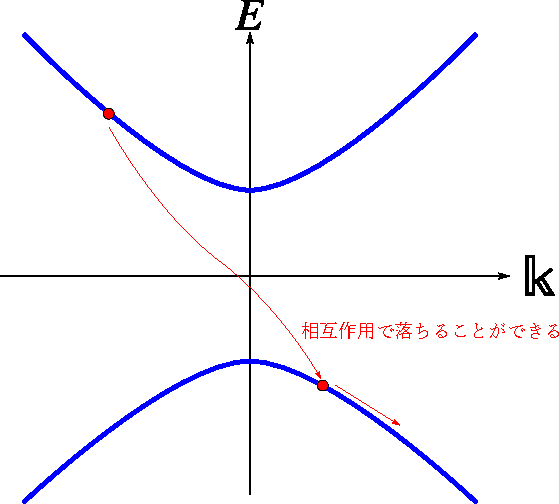
\includegraphics{negative_energy.pdf}
  \caption{Dirac方程式のエネルギー準位の様子。青いところが電子が入れる状態がある部分。相互作用があると最初正エネルギーのところにいても負エネルギーのところに遷移することがあり、さらにいくらでも負で大きいエネルギーのところに落ちていってしまう。}
  \label{fig:negative_energy}
\end{figure}

Diracはこの困難に対して次のような解決法を提案しました。ミソは電子がフェルミオンであることです。フェルミオンはPauliの排他律と呼ばれる、同じ状態に2つの粒子が入れないという法則があります。これを考えに入れて、すべての負のエネルギー準位が埋め尽くされている状態が「真空」と考えるべきだ、というのがDiracの提案です。このような負のエネルギーが電子で埋め尽くされていることを\strong{Diracの海}と言います。この提案が良いことの1つの理由は、負のエネルギー準位は、そこに電子がいるとエネルギーが下がりますから、埋め尽くされているがエネルギー最小となり、「真空」と呼ぶにふさわしい状態になります。「真空」以外の状態は、すべて「真空」よりもエネルギーが高くなります。
\begin{figure}[htbp]
  \centering
  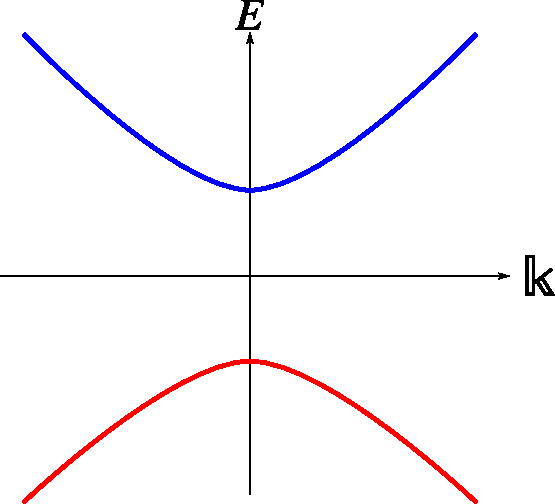
\includegraphics{diracsea.pdf}
  \caption{Diracの提案した真空状態。すべての負エネルギー準位に電子が詰まっているのを赤く表している。}
  \label{fig:diracsea}
\end{figure}

真空状態に比べて、余分に正のエネルギー準位の1つが埋まっている状態が1つの電子がある状態と言えます。図\ref{fig:oneparticle}を見てください。今度は、先程のケースと異なり、電子は負のエネルギー状態に行くことができません。それは、負のエネルギー準位は既にすべて埋まっており、Pauliの排他律により他の電子が入ってくることができないからです。したがって、このような状態は安定な状態となります。
\begin{figure}[htbp]
  \centering
  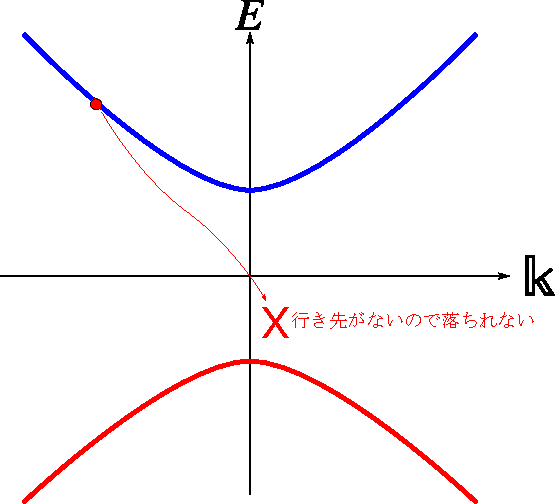
\includegraphics{oneparticle.pdf}
  \caption{1つの電子がある状態。負のエネルギー準位はすべて埋まっているので、Pauliの排他律のため落ちることができない。}
  \label{fig:oneparticle}
\end{figure}

Diracの提案がすごいのは、ここからです。図\ref{fig:antiparticle}のように、負エネルギー準位の電子が1つ足りないような状態を考えることができます。これは、どのような状態でしょうか。これは、真空状態に比べて「負のエネルギー」の電子が「足りない」ので、正のエネルギーを持つことになります。また、この準位の運動量が足りないので、その反対の運動量を持つことになります。角運動量も同様です。特に電荷は電子の電荷の逆になります。このような状態を「陽電子」が1つある状態と呼ぶことができると思います。今は電子を考えたので陽電子が出てきましたが、ここでの議論を一般の粒子にあてはめると、必ず質量が同じで電荷などの量子数が逆になるような粒子が出てくることになります。このような粒子のことを\strong{反粒子}と呼びます。つまり電子の反粒子は陽電子になります。
\begin{figure}[htbp]
  \centering
  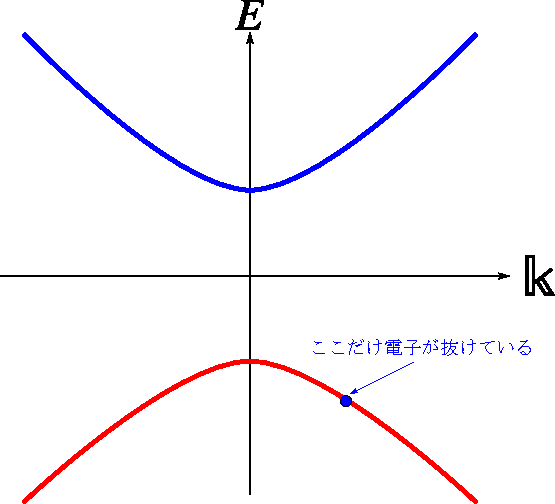
\includegraphics{antiparticle.pdf}
  \caption{負エネルギー状態の電子が1つ抜けた状態。電子の反粒子である「陽電子」が1つある状態と言える。}
  \label{fig:antiparticle}
\end{figure}

さらにこれを推し進めると、次のような現象を予言することができます。図\ref{fig:paircreation}の左のように電子と陽電子が1つずつあるような状態を考えてみます。この場合、正エネルギーを持つ電子が空いている負エネルギー準位に落ち込むことができ、この遷移で放射を出します。結果、電子も陽電子もなくなり放射だけがあるような状態になりました。このような変化を\strong{対消滅}と呼びます。逆に何かの拍子に負エネルギー状態に詰まっている電子が放射のエネルギーを吸収して正エネルギーへと励起すると左側の電子と陽電子が1つずつある状態になります。このような変化を\strong{対生成}と呼びます。
\begin{figure}[htbp]
  \centering
  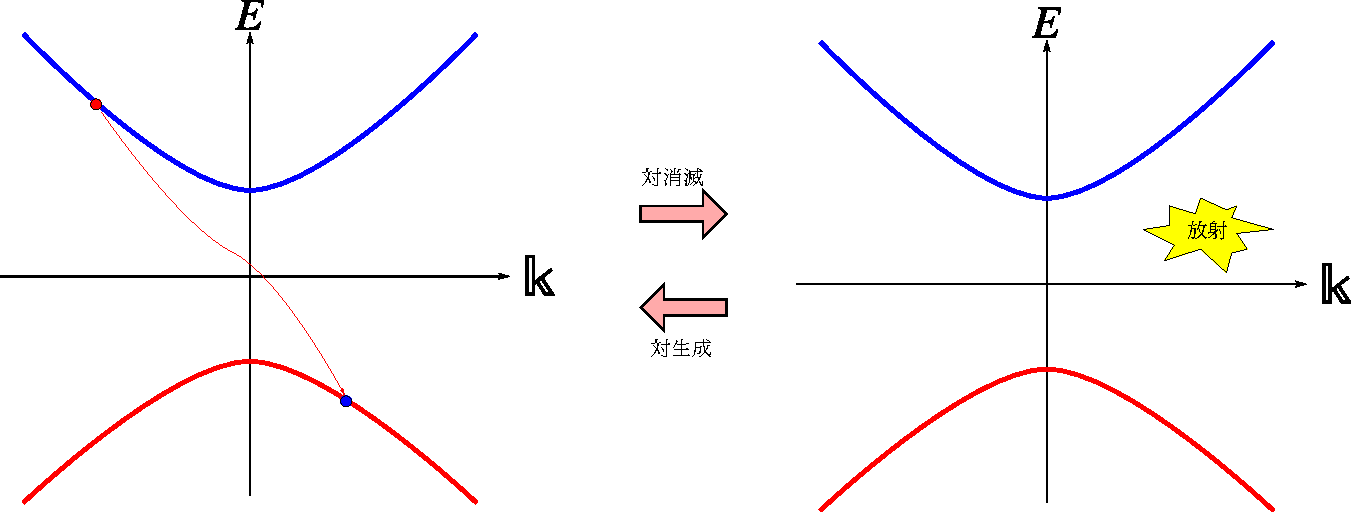
\includegraphics[width=14cm]{paircreation.pdf}
  \caption{対生成と対消滅}
  \label{fig:paircreation}
\end{figure}

このようにしてDiracは陽電子などの反粒子を予言し、それらが対生成や対消滅などの反応をすることを予言しました。実際に陽電子は、すぐに発見し、Diracの海の描像が正しいことが示されました。

このようにDirac方程式とDiracの海の見方は大成功しましたが、同時に1粒子を記述する方程式としてのDirac方程式の限界も示しました。Diracの海を表すためには、1粒子だけ記述するというのは本質的に限界があり、無限個の粒子を記述しなければなりません。別の言い方をするなら、対生成や対消滅といった粒子の数が変化するような時間発展を記述できるような理論の枠組みでなければ、正しく自然界を記述できていないことになります。

したがって、量子力学を相対論的に書き換えようとすれば、必然的に粒子の数や種類の変化も含めて記述できる理論である\strong{場の理論}に行かなければなりません。この講義の後半では、場の理論の入門的な説明をします。大学院では、本格的に場の理論を取り扱う講義があります。

この講義の前半では、1粒子の電子を記述する理論としてのDirac方程式を学びます。この記述は対生成や対消滅が起こらない範囲内で近似的に1つの電子を記述する理論としては、よいものです。

\section{Maxwell方程式}
重要な相対論的な場の方程式であり、みなさんにも馴染み深いものがMaxwell方程式です。これも自然界の記述に重要な役割を果たすので、ここで触れておきます。物質がない場合のMaxwell方程式はベクトル場$A_{\mu}(x)$に対する方程式で
\begin{align}
  \del_{\mu}(\del^{\mu}A^{\nu}-\del^{\nu}A^{\mu})=0
\end{align}
と書けます。

これの特徴は次のとおりです。
\begin{itemize}
  \item 明白なLorentz不変性があります。
  \item 1粒子の量子力学の波動関数としては解釈できません。
  \item 相対論的な場の方程式としては良いものです。光子と呼ばれる粒子の元になる場を記述します。
\end{itemize}

ここで少し、力と物質ということについて考えてみたいと思います。
そもそも電磁気という「力」を記述するために、場の概念が導入されました。
みなさんがこれまで習ってきたように、Maxwell理論による電磁場の記述は大変良いものです。
一方で前の節で見たように、物質を記述する際にも場の導入が必然でした。
つまり、力と物質という、力学では全く異なる意味を持つ2つの物理の概念が、ここまで来ると「場」という同じ概念で表されることになります。
つまり、\strong{場の理論においては「力」と「物質」は両方「場」であり、同じ土俵で記述できます。}


\section{この章のまとめ}
この章では、量子力学を相対論的に書きかえるという様々な試みを紹介してきました。
\begin{itemize}
  \item 古典的な粒子の正準形式の理論を素朴に量子化したものは、うまくいきません。
  \item Klein-Gordon方程式は、明白なLorentz不変性を持ちます。しかし、保存する「確率」は負にもなりうるため、確率解釈はできません。負エネルギー解もあります。
  \item Dirac方程式は、明白なLorentz不変性を持ち、確率解釈も可能です。しかし負エネルギー解を持ちます。
  \item Diracの海の描像により、反粒子の存在が予言されます。
  \item 量子力学を相対論的に書きかえようとすると、必然的に場の理論に行かないといけないことが分かります。
  \item Klein-Gordon方程式、Dirac方程式、Maxwell方程式は相対論的な場の方程式として良いものです。
\end{itemize}

\chapter{Dirac方程式}
\section{ガンマ行列}
Dirac方程式\eqref{freeDiracequation}をもう一度書きます。
\begin{align}
  i\del_{0}\psi=(-i\alpha_i\del_{i}+m\beta)\psi.
  \label{freeDiracequation1}
\end{align}
これは、時間微分は左辺にあって空間微分は右辺にあったりするので、もう少し時間と空間を平等に扱った形に書き換えます。ガンマ行列$\gamma^{\mu}$を
\begin{align}
  \gamma^{0}=\beta,\quad \gamma^{i}=\beta\alpha_i
\end{align}
とすると、Dirac方程式\eqref{freeDiracequation1}は
\begin{important}
  \begin{align}
    (i\gamma^{\mu}\del_{\mu}-m)\psi=0 \label{freeDiracequation2}
  \end{align}
\end{important}
という形に書くことができます。こちらの方が少なくともベクトルの添字を$\mu=0,1,2,3$の縮約で書いているので見た目が良いです。実際、例えば場の理論でDirac方程式を扱う場合、こちらの形の方が遥かに便利です。

ここで出てきたガンマ行列$\gamma^{\mu}$は、
\begin{important}
  \begin{align}
    \{\gamma^{\mu},\gamma^{\nu}\}=2\eta^{\mu\nu}\label{gammaanticommutationrelation}
  \end{align}    
\end{important}
という反交換関係を満たします。この形の反交換関係は記憶に便利ですが、実際に計算するときには、次のように、ばらした形の方が便利な場合も多いです。
\begin{align}
  (\gamma^{0})^2=1,\quad (\gamma^{i})^2=-1,\quad
  \gamma^{\mu}\gamma^{\nu}=-\gamma^{\nu}\gamma^{\mu}\ (\mu\ne \nu).
  \label{gammaanticommutationrelation1}
\end{align}
また、$\alpha_i,\beta$がエルミートであることから
\begin{align}
  \gamma^{0\dag}=\gamma^{0},\quad \gamma^{i\dag}=-\gamma^{i}
  \label{gammahermiticity}
\end{align}
となります。

この表記の有用性を示すために、Dirac方程式の確率の保存を考えてみましょう。
まず、Dirac共役$\psib$を
\begin{important}
  \begin{align}
    \psib:=\psi^{\dag}\gamma^{0}
  \end{align}  
\end{important}
で定義します。$\psib$は4成分を横にならべたものであることに注意してください。後々見ていくようにエルミート共役ではなく、このDirac共役を用いることにより、様々な式を共変に書くことができます。

次のような4元反変ベクトルっぽい量を定義します\footnote{本当に4元反変ベクトルであることは、後に$\psi$のLorentz変換がどうなるかを調べたあとで示します。}。
\begin{align}
  j^{\mu}=\psib \gamma^{\mu}\psi.
\end{align}
成分を見てみると時間成分が以前導入した確率密度、空間成分が確率の流れ密度になります。

$j^{\mu}$が連続の式$\del_{\mu}j^{\mu}=0$を満たすことを示しましょう。まず、反交換関係\eqref{gammaanticommutationrelation}あるいは\eqref{gammaanticommutationrelation1}とエルミート共役の関係\eqref{gammahermiticity}を用いると
\begin{align}
  \gamma^{0}\gamma^{\mu\dag}\gamma^{0}=\gamma^{\mu}\label{gammahermiticity2}
\end{align}
を得ます。Dirac方程式\eqref{freeDiracequation2}の両辺のエルミート共役をとり、式\eqref{gammahermiticity2}を用いると
\begin{align}
  \psib(-i\gamma^{\mu}\dell_{\mu}-m)=0\label{conjugateDiraceqation}
\end{align}
を得ます。ここで記述の簡単のために左側に作用する微分演算子$\dell_{\mu}$を導入しました。$\psib\dell_{\mu}:=\del_{\mu}\psib$です。式\eqref{freeDiracequation2}と式\eqref{conjugateDiraceqation}を用いると
\begin{align}
  \del_{\mu}j^{\mu}&=\del_{\mu}(\psib\gamma^{\mu}\psi)
  =\psib\gamma^{\mu}\dell_{\mu}\psi+\psib\gamma^{\mu}\del_{\mu}\psi\nonumber\\
  &=\psib(im)\psi+\psib(-im)\psi=0
\end{align}
となって、保存の式$\del_{\mu}j^{\mu}=0$が示せます。

\section{スピン}
Dirac方程式の一番美しいところは、非相対論的な場合には手で入れていた電子の「スピン」が必然的に入っているところです。これについて見ていきましょう。

まず、軌道角運動量について思い出してください。3次元ベクトルの外積の記号で
\begin{align}
  \Lb=\xb \times \pbb=-i\xb\times\bnabla
\end{align}
でした。3次元の成分では、
\begin{align}
  L_i=-i\epsilon_{ijk}x^{j}\del_{k}
\end{align}
と書けます。ここで$\epsilon_{ijk}$は完全反対称テンソルで$\epsilon_{123}=1$となる記号です。

軌道角運動量が保存するかどうかを見てみましょう。これにはHamiltonian\eqref{DiracHamiltonian}と交換するかどうかを見ればよいです。交換関係は
\begin{align}
  [H,L_i]=-\epsilon_{ijk}\alpha_{j}\del_{k}\label{HLi}
\end{align}
となります。したがって\strong{軌道角運動量は保存しない}ということが分かります。

これはどういうことでしょうか。角運動量は回転対称性の保存量でしたから、それが保存しないということは、回転対称性がないということでしょうか。答えは、軌道角運動量以外にスピンという角運動量があって、合わせると保存していて回転対称性はちゃんと保っている、というものです。少々天下り的ですが、スピンを
\begin{align}
  S_i
  :=\frac{i}{4}\epsilon_{ijk}\gamma^{j}\gamma^{k}
  :=-\frac{i}{4}\epsilon_{ijk}\alpha_{j}\alpha_{k}\label{spin1/2}
\end{align}
と定義します。具体的に成分を書くと
\begin{align}
  S_1=-\frac{i}{2}\alpha_{2}\alpha_{3},\quad
  S_2=-\frac{i}{2}\alpha_{3}\alpha_{1},\quad
  S_3=-\frac{i}{2}\alpha_{1}\alpha_{2},\quad
\end{align}
となります。このとき、次の2つのことが成り立ちます。
\begin{itemize}
  \item $S_i$が角運動量の交換関係を満たすこと。
  \item 軌道角運動量とスピンをあわせた全角運動量$L_i+S_i$が保存すること。
\end{itemize}

まず、角運動量の交換関係を満たすことを確かめましょう。例えば
\begin{align}
  [S_1,S_2]&=-\frac{1}{4}[\alpha_{2}\alpha_{3},\alpha_{3}\alpha_{1}]
  =-\frac{1}{4}(\alpha_{2}\alpha_{3}\alpha_{3}\alpha_{1}-\alpha_{3}\alpha_{1}\alpha_{2}\alpha_{3})\nonumber\\
  &=-\frac{1}{4}(\alpha_{2}\alpha_{1}-\alpha_{1}\alpha_{2})
  =\frac{1}{2}\alpha_{1}\alpha_{2}
  =iS_3
\end{align}
となります。計算には式\eqref{alphabeta}の関係を用いました。$1,2,3$を巡回的に入れ替えれば、結局
\begin{align}
  [S_i,S_j]=i\epsilon_{ijk}S_k
\end{align}
という角運動量の交換関係が成り立つことが分かりました。

次に$L_i+S_i$が保存することを確かめましょう。まず式\eqref{alphabeta}の関係を用いて交換関係$[H,S_i]$を計算します。例えば
\begin{align}
  [H,S_1]
  =[-i\alpha_i\del_i+m\beta,-\frac{i}{2}\alpha_2\alpha_3]
  =-\frac12\del_{i}[\alpha_i,\alpha_2\alpha_3]
  =-\del_{2}\alpha_{3}+\del_{3}\alpha_{2}
\end{align}
となります。$1,2,3$を巡回的に入れ替えると
\begin{align}
  [H,S_i]=\epsilon_{ijk}\alpha_{j}\del_{k}
\end{align}
を得ます。\eqref{HLi}と合わせると
\begin{align}
  [H,L_i+S_i]=0
\end{align}
が確かめられました。

さて、「スピンの大きさ」を求めておきましょう。
\begin{align}
  \Sb^2=\sum_{i}S_i^2=\frac{3}{4}=\frac{1}{2}\qty(\frac{1}{2}+1)=s(s+1)
\end{align}
なので、$s=\frac{1}{2}$となります。つまり、Dirac方程式はスピン$\frac{1}{2}$の粒子を記述しています。例えば、電子はスピン$\frac{1}{2}$なのでDirac方程式でうまく記述できます。

\section{Lorentz変換}
Dirac方程式\eqref{freeDiracequation2}は、Lorentz不変になりそうな雰囲気ではありますが、これまではちゃんとLorentz不変であることを示していませんでした。Lorentz不変であることを示すためには、4成分の$\psi$がLorentz変換の元でどう振る舞うかを考える必要があります。$\psi$は4成分の場ですが、ベクトルではありません。このような場は\strong{スピノール}と呼ばれます。スピノールがLorentz変換でどのように振る舞うかを調べるのがここでの目的です。

\subsection{3次元の回転}
まず、ウォーミングアップとしてLorentz変換の一部である3次元の回転を復習しましょう。ここではLie群、Lie代数、表現論といった数学の概念が有用ですので、簡単に説明します。こういった数学は場の理論、特にゲージ理論を考える際に不可欠ですので、みなさん勉強してください。

3次元の回転は$3\times 3$行列$R$で$RR^{T}=1,\ \det R=1$を満たすようなものです。こういう変換の集合は、次のような性質を持っています。
\begin{enumerate}
  \item 行列の集合は結合則を満たす掛け算で閉じています。
  \item 単位元$1$があります。
  \item この集合の任意の元$R$に対して、「逆元」$R^{-1}$が存在します。
\end{enumerate}
一般にこの3つの性質を持つ集合を\strong{群}と呼びます。群は対称性を表すのに便利な数学の概念です。
群のうち「連続的なもの」をLie群と呼びます。大事なことは、群を考えるときは抽象的な掛け算の構造だけに注目し、どのような行列で表されていたかというのは一旦忘れることです。具体的に群の元を掛け算の構造を保ったまま行列で表すことを\strong{表現}と呼びます。\strong{1つの群に対していろんな表現がある}、ということが非常に重要です。実際、量子力学では状態に対して回転がどう作用するか、ということを考えるわけですが、これは回転の群を$\infty\times\infty$の行列で表すことに対応しています。

量子力学でよくやるように、無限小変換を考えましょう。$R$が非常に$1$に近いとき、ある非常に小さい数$\theta_i \ (i=1,2,3)$を用いて
\begin{align}
  R=1-i\theta_i J_i
\end{align}
と書けます。ここで$J_i$は生成子と呼ばれるもので
\begin{align}
  J_1=\mqty(
    0 & 0 & 0\\
    0 & 0 & -i\\
    0 & i & 0
  ),\quad
  J_2=\mqty(
    0 & 0 & i\\
    0 & 0 & 0\\
    -i & 0 & 0
  ),\quad
  J_3=\mqty(
    0 & -i & 0\\
    i & 0 & 0\\
    0 & 0 & 0
  )\label{so(3)3rep}
\end{align}
とします。群では、掛け算の構造が重要でしたが、それを無限小変換の言葉になおすと交換関係になります。
交換関係は、実際に計算すると
\begin{align}
  [J_i,J_j]=i\epsilon_{ijk}J_k\label{so(3)alg}
\end{align}
となります。この$J_i$の線形結合全体で表される集合は次の性質を持っています。
\begin{enumerate}
  \item ベクトル空間です。つまり、足し算とスカラー倍があり、所定の性質を持っています。
  \item 双線形な演算$[,]$があります。
  \item この集合の任意の元$X,Y$に対して$[X,Y]=-[Y,X]$を満たします。
  \item この集合の任意の元$X,Y,Z$に対して$[X,[Y,Z]]+[Z,[X,Y]]+[Y,[Z,X]]=0$(Jacobi恒等式)を満たします。
\end{enumerate}
一般に、このような性質を満たす集合を\strong{Lie代数}と呼びます。Lie代数は、連続的な対称性の無限小変換の性質を考えるための数学的な対象として非常に有用なものです。やはり、ここでも大事なことは、\eqref{so(3)3rep}のような具体的に行列でどう表されるかは一旦忘れ、Lie代数の構造である線形結合や交換関係\eqref{so(3)alg}にのみ注目することです。線形結合や交換関係の構造を保つように行列で表すことを\strong{表現}と呼びます。やはり1つのLie代数に対して、いろんな表現があります。例えば皆さんは回転のLie代数の表現として$2\times 2$の行列で表す方法を知っていると思います。つまり、Pauli行列$\sigma_i$を用いて$J_i=\frac12\sigma_i$とすれば、交換関係\eqref{so(3)alg}を満たします。他のいろんな次元の表現を作る方法を量子力学の授業でやったと思います。

ここでは、Lie群やLie代数について、これ以上詳しくやる時間は残念ながらありません。自分たちで本などを読んで勉強することを強く勧めます。

さて、物理に戻りましょう。これまで準備してきた数学を用いると、次のように言えます。
\begin{myquote}
  角運動量とは空間回転のLie代数のHilbert空間に対する表現である。
\end{myquote}
つまり、\eqref{so(3)alg}の交換関係を満たすようなHilbert空間上の演算子です。例えば、非相対論的でスピンを持たない粒子の場合、Hilbert空間は3次元空間での規格化可能な関数全体でした。その場合の角運動量は
\begin{align}
  J_i=L_i:=-i\epsilon_{ijk}x^j\del_{k}
\end{align}
となります\footnote{ここでは、記号の簡単のためにLie代数の元とその表現に同じ記号$J_i$を用いました。これはもしかしたら混乱を招くかもしれません。繰り返しますが、抽象的なLie代数の元とその表現を区別することが非常に重要です。}。この$L_i$のことを物理では軌道角運動量と呼んでいるわけです。同様にDirac方程式で記述される4成分の波動関数$\psi(x)$に対しては、前の節でやったように
\begin{align}
  J_i=L_i+S_i,\quad S_i=\frac{i}{4}\epsilon_{ijk}\gamma^{j}\gamma^{k}\label{3dangularmomentum}
\end{align}
となります。これが\eqref{so(3)alg}の交換関係を満たすことは前節で確かめました。

\subsection{Lorentz群とそのLie代数}
さて、前項でやったことをLorentz変換のなす群でやります。まず、Lorentz変換全体が群をなすことは良いでしょうか。結合則が成り立つ掛け算があって、単位元、逆元があるような集合を群と言うのでした。Lorentz変換全体は、「変換を続けて行う」というのを掛け算とすると、この性質を満たします。これをLorentz群と呼んでおくことにしましょう。Lorentz群を考えることは、3次元の回転を考えることに比べて次の2点で難しくなっています。
\begin{itemize}
  \item 3次元が4次元になっている。
  \item (ベクトルの大きさ)${}^2$が必ずしも正ではない。
\end{itemize}
逆に言えば、これ以外は変わっていません。変わったところ、変わっていないところに注目して読んでいってください。

具体的に付録\ref{app:tensor}の記号を使って説明します。Lorentz変換は$x'^{\mu}=\Lambda^{\mu}{}_{\nu}x^{\nu}$という1次変換で表されます。ここで$\Lambda^{\mu}{}_{\nu}$は
\begin{align}
  \eta_{\mu\nu}\Lambda^{\mu}{}_{\rho}\Lambda^{\nu}{}_{\sigma}=\eta_{\rho\sigma}
  \label{Lorentztransf1}
\end{align}
という関係を満たします。

さて、Lorentz変換の無限小変換を考えることにより、Lorentz群のLie代数(Lorentz代数と呼んでおきましょう)の構造を考えます。$\omega^{\mu}{}_{\nu}$を非常に小さい量として
\begin{align}
  \Lambda^{\mu}{}_{\nu}=\delta^{\mu}_{\nu}+\omega^{\mu}{}_{\nu}\label{infinitesimalLorentz0}
\end{align}
を考えます。この$\omega^{\mu}{}_{\nu}$が満たすべき性質を調べましょう。式\eqref{Lorentztransf1}に\eqref{infinitesimalLorentz0}を代入して変形し、$\omega$の2次以上を無視します。
\begin{align}
  &\eta_{\mu\nu}(\delta^{\mu}_{\rho}+\omega^{\mu}{}_{\rho})(\delta^{\nu}_{\sigma}+\omega^{\nu}{}_{\sigma})=\eta_{\rho\sigma}\\
  \Leftrightarrow\quad&\eta_{\mu\nu}\delta^{\mu}_{\rho}\delta^{\nu}_{\sigma}+\eta_{\mu\nu}\delta^{\mu}_{\rho}\omega^{\nu}{}_{\sigma}+\eta_{\mu\nu}\omega^{\mu}{}_{\rho}\delta^{\nu}_{\sigma}=\eta_{\rho\sigma}\\
  \Leftrightarrow\quad&\eta_{\rho\sigma}+\omega_{\rho\sigma}+\omega_{\sigma\rho}=\eta_{\rho\sigma}
\end{align}
と変形できます。$\eta_{\mu\nu}\omega^{\nu}{}_{\sigma}=:\omega_{\mu\sigma}$と定義しました。得られたのは
\begin{important}
  \begin{align}
    \omega_{\rho\sigma}=-\omega_{\sigma\rho}\label{infinitesimalLorentz1}
  \end{align}
  つまり、(無限小Lorentz変換のパラメータ)$=$(反対称テンソル)。
\end{important}
ということです
%\footnote{例えば$\Lambda$がテンソルか否かということは議論できません。なぜなら、$\Lambda$は1つの座標系が決まれば決まるというものではないからです。しかし、$\omega$は無限小変換ですからテンソルか否かが議論できて、ここでは本当にテンソルになります。}
。3次元の回転のときは、無限小変換のパラメータは$\theta_i$という3次元ベクトルでした。この違いは3次元と4次元の違いに起因します。というより、一般には、反対称テンソルで、3次元の場合に限って(反対称テンソル)$=$(ベクトル)という関係が成り立ってしまうのです。つまり
\begin{align}
  \theta_{i}=\frac12 \epsilon_{ijk}\omega_{jk}
\end{align}
という関係があります。テンソルというと難しく感じるので、これまで物理の授業ではベクトルとして習ってきたのです。

次にLorentz変換の生成子について考えましょう。数学の言葉では生成子はLie代数の(ベクトル空間としての)基底です。式\eqref{infinitesimalLorentz1}の関係を用いると、\eqref{infinitesimalLorentz0}は
\begin{align}
  \Lambda^{\mu}{}_{\nu}=\delta^{\mu}_{\nu}-\frac{i}{2}\omega^{\rho\sigma}(M_{\rho\sigma})^{\mu}{}_{\nu}
\end{align}
と書けます。ここで
\begin{align}
  (M_{\rho\sigma})^{\mu}{}_{\nu}:=i\delta^{\mu}_{\rho}\eta_{\sigma\nu}-i\delta^{\mu}_{\sigma}\eta_{\rho\nu}\label{vectorrep0}
\end{align}
を導入しました。括弧をつけた変な書き方をしている理由は、$M_{\rho\sigma}$というのが、($\rho,\sigma$を固定したときに)$4\times 4$の行列と思いたいからです。足の付き方も、ちゃんと掛け算できる付き方になってますよね。$M_{\rho\sigma}=-M_{\sigma\rho}$ですから、独立な生成子は$M_{01},\ M_{02},\ M_{03},\ M_{12},\ M_{23},\ M_{13}$の6つです。繰り返しますが、これら1つ1つが$4\times 4$行列であることに注意してください。例えば
\begin{align}
  M_{12}=\mqty(
    0 & 0 & 0 & 0 \\  
    0 & 0 & -i & 0 \\  
    0 & i & 0 & 0 \\  
    0 & 0 & 0 & 0 \\  
  ),\quad
  M_{01}=\mqty(
    0 & -i& 0 & 0 \\  
    -i& 0 & 0 & 0 \\  
    0 & 0 & 0 & 0 \\  
    0 & 0 & 0 & 0 \\  
  )
\end{align}
などです。ただし、ここでは$(M_{\rho\sigma})^{\mu}{}_{\nu}$の$\mu$を行の足、$\nu$を列の足にし、それぞれ$0,1,2,3$の順で書きました。
独立な生成子が6つあるという意味でLorentz群、およびそのLie代数は6次元です。例えば$M_{12}$は$0$行および$0$列を除くと、全体の符号を除いて\eqref{so(3)3rep}の$J_3$と同じになっています。これは当然で、3次元の回転はLorentz変換の特別な場合です。$M_{01}$などが、速度の違う観測者に移るという、Lorentz変換らしいLorentz変換であり、「ブースト」と呼ばれます。ブーストの生成子は行列としては反対称行列ではなく対称行列(エルミート行列ではなく、反エルミート行列)になっていますが、この違いは「(大きさ)${}^2$が必ずしも正ではない。」の方の違いから来ています。

さて、Lie代数の構造で重要なのは、交換関係でした。生成子の交換関係を計算しましょう。答えは
\begin{important}
  \begin{align}
    [M_{\mu\nu},M_{\rho\sigma}]=i\eta_{\nu\rho}M_{\mu\sigma}-i\eta_{\mu\rho}M_{\nu\sigma}
    +i\eta_{\mu\sigma}M_{\nu\rho}-i\eta_{\nu\sigma}M_{\mu\rho}\label{Lorentzcomm}
  \end{align}
\end{important}
となります。この式は、その内容以上に見た目がゴチャゴチャしていて難しく感じてしまうと思います。計算は強引にやればできますが、うまくやらないと面倒です。少しだけ「計算しなくても分かること」を解説しましょう。
\begin{itemize}
  \item Lie代数になっていることを認めると、交換関係は$M$ついて1次のはずです。
  \item 交換関係の結果に現れるテンソルは$M_{\cdot\cdot}$と$\eta_{\cdot\cdot},\eta^{\cdot\cdot}$および$\delta^{\cdot}_{\cdot}$というものだけのはずです。これらを用いて下付きの足を$4$つもつもので$M$について1次のものものは、$\eta_{\cdot\cdot}M_{\cdot\cdot}$で$\cdot$のところには$\mu\nu\rho\sigma$を順番を入れ替えていれたものという組み合わせしかありません。
  \item さらに$M_{\mu\nu}$は$\mu\nu$について反対称ですから、左辺の交換関係は$\mu\nu$および$\rho\sigma$については反対称なはずです。したがって、$\eta_{\mu\nu}M_{\rho\sigma}$のような項はありえません。この反対称性まで考慮すると「計算しなくても」全体にかかる係数を除いて式\eqref{Lorentzcomm}と一致することが分かります。
\end{itemize}
全体にかかる係数を決めるには、例えば$[M_{12},M_{31}]$を計算すれば、式\eqref{Lorentzcomm}の第3項だけが$0$でなく出てくるので、その係数を見れば良いです。

\subsection{スカラー場への表現}
まずは、練習のためにスカラー場$\phi(x)$への表現を考えましょう。スカラー場はLorentz変換のもとで
\begin{align}
  \phi'(x')=\phi(x)\label{scalartransf0}
\end{align}
と変換します。無限小変換のもとでは、$x$は
\begin{align}
  x'^{\mu}=(\delta^{\mu}_{\nu}+\omega^{\mu}{}_{\nu})x^{\nu}=x^{\mu}+\omega^{\mu}{}_{\nu}x^{\nu}
\end{align}
と変換します。ひとまず
\begin{align}
  x'^{\mu}=x^{\mu}+\delta x^{\mu},\quad \delta x^{\mu}:=\omega^{\mu}{}_{\nu}x^{\nu}
\end{align}
と書いておきましょう。
このとき、スカラー場の変化$\delta \phi(x):=\phi'(x)-\phi(x)$を計算しましょう。引数が同じ$x$であることに注意してください。式\eqref{scalartransf0}を用いて計算すると
\begin{align}
  \delta \phi(x)&:=\phi'(x)-\phi(x)=\phi'(x'-\delta x)-\phi(x)\nonumber\\
  &=\phi'(x')-\delta x^{\mu}\del_{\mu}\phi(x)-\phi(x)
  =-\omega^{\mu}{}_{\nu}x^{\nu}\del_{\mu}\phi(x)
  =-\frac{i}{2}\omega^{\mu\nu}L_{\mu\nu}\phi(x)\label{scalarinfinitesimaltransf}
\end{align}
となります。ここで$\omega$の2次以上は無視しました。また$L_{\mu\nu}$は
\begin{align}
  L_{\mu\nu}=i(x_{\mu}\del_{\nu}-x_{\nu}\del_{\mu})
\end{align}
と定義しました。この$L_{\mu\nu}$の交換関係を計算すると\eqref{Lorentzcomm}と同じになることが分かります。つまり
\begin{align}
  [L_{\mu\nu},L_{\rho\sigma}]=i\eta_{\nu\rho}L_{\mu\sigma}-i\eta_{\mu\rho}L_{\nu\sigma}
  +i\eta_{\mu\sigma}L_{\nu\rho}-i\eta_{\nu\sigma}L_{\mu\rho}
\end{align}
となります。言い換えると、$L_{\mu\nu}$はLorentz代数の表現になっています。

ここで出てきた$L_{\mu\nu}$は、見た目のとおり軌道角運動量のアナロジーです。スカラー場の場合には$L_{\mu\nu}$以外の部分、つまりスピンはありません。言い換えると、スカラー場はスピン0です。


スカラー場の場合に、無限小変換から有限変換を導出できることを見ておきましょう。この部分に関しては、3次元の量子力学でやったことと難しさは変わりません。
無限小変換\eqref{scalarinfinitesimaltransf}から有限にするには、指数関数をとって
\begin{align}
  \phi'(x)=\exp\qty(-\frac{i}{2}\omega^{\rho\sigma}L_{\rho\sigma})\phi(x)\label{scalartransf1}
\end{align}
とすれば良いです。


変換\eqref{scalartransf0}と\eqref{scalartransf1}が同じであることを証明するには、次のようにします。
まず、\eqref{vectorrep0}の表現(「ベクトル表現」と呼ばれます)を$V$で表すことにします。つまり
\begin{align}
  (V_{\rho\sigma})^{\mu}{}_{\nu}:=i\delta^{\mu}_{\rho}\eta_{\sigma\nu}-i\delta^{\mu}_{\sigma}\eta_{\rho\nu}
\end{align}
とします。$M$は表現を忘れた抽象的なLie代数の生成子ということにしておきます。有限変換の群の元のベクトル表現は$\omega^{\rho\sigma}$を有限として
\begin{align}
  \Lambda^{\mu}{}_{\nu}=\qty(\exp\qty(-\frac{i}{2}\omega^{\rho\sigma}V_{\rho\sigma}))^{\mu}{}_{\nu}\label{finiteomega}
\end{align}
と指数関数をとることで得られます。逆行列は
\begin{align}
  (\Lambda^{-1})^{\mu}{}_{\nu}=\qty(\exp\qty(\frac{i}{2}\omega^{\rho\sigma}V_{\rho\sigma}))^{\mu}{}_{\nu} 
\end{align}
となります。次に\eqref{scalartransf0}は次のように書き直すことができます。
\begin{align}
  \phi'(x)=\phi(\Lambda^{-1}x)=\phi\qty(\qty(\exp\qty(\frac{i}{2}\omega^{\rho\sigma}V_{\rho\sigma}))x).
\end{align}
さて$0\le u \le 1$をとるパラメータを導入して
\begin{align}
  \phi'_{u}(x):=\exp\qty(-u\frac{i}{2}\omega^{\rho\sigma}L_{\rho\sigma})\phi(x),\label{tempphiprime}\\
  \phit_{u}(x):=\phi\qty(\qty(\exp\qty(u\frac{i}{2}\omega^{\rho\sigma}V_{\rho\sigma}))x)\label{tempphitilde}
\end{align}
を定義します。これから$\phi'_{u}(x)=\phit_{u(x)}$を示します。$u=1$の場合が示したかった式です。これを示すのには、次の2つを示せば良いです。
\begin{enumerate}
  \item $u=0$のとき$\phi'_{0}(x)=\phit_{0}(x)$であること。
  \item $\phi'_{u}(x)$と$\phit_{u}(x)$が同じ微分方程式を満たすこと。
\end{enumerate}
まず、$\phi'_{0}(x)=\phit_{0}(x)=\phi(x)$ですから1.は成り立ちます。次に$\phi'_{u}(x)$が満たす微分方程式を求めましょう。式\eqref{tempphiprime}より
\begin{align}
  \pdv{u} \phi'_{u}(x)=-\frac{i}{2}\omega^{\rho\sigma}L_{\rho\sigma}\phi'_{u}(x)\label{tempdiffeqprime}
\end{align}
となります。次に$\phit_{u}(x)$が満たす微分方程式を求めましょう。$\delta u$を小さい数、$B:=\qty(\exp\qty(\frac{i}{2}\omega^{\rho\sigma}V_{\rho\sigma}))$とすると、$\phi_u(x)=\phi(B^ux)$と書けます。さらに$B^{\delta u}x=x+\delta x$と書くことにすると
\begin{align}
  \phit_{u+\delta u}(x)
  =\phi(B^{u+\delta u}x)
  =\phi(B^{u}B^{\delta u}x)\nonumber\\
  =\phit_u(B^{\delta u}x)
  =\phit_u(x)+\delta x^{\mu}\del_{\mu}\phit_{u}(x)\label{tempdiffeq0}
\end{align}
となります。ところで、ここで導入した$\delta x$をもう少し計算すると
\begin{align}
  \delta x^{\mu}\del_{\mu}=\delta u\frac{i}{2}\omega^{\rho\sigma}(V_{\rho\sigma})^{\mu}{}_{\nu}x^{\nu}\del_{\mu}
  =-\delta u\frac{1}{2}\omega^{\rho\sigma}\qty(\delta^{\mu}_{\rho}\eta_{\nu\sigma}-\delta^{\mu}_{\sigma}\eta_{\nu\rho})x^{\nu}\del_{\mu}\nonumber\\
  =-\delta u\frac{1}{2}\omega^{\rho\sigma}\qty(x_{\sigma}\del_{\rho}-x_{\rho}\del_{\sigma})
  =-\delta u \frac{i}{2}\omega^{\rho\sigma}L_{\rho\sigma}
\end{align}
となるので式\eqref{tempdiffeq0}は
\begin{align}
\phit_{u+\delta u}(x)=\phit_{u}(x) - \delta u\frac{i}{2}\omega^{\rho\sigma}L_{\rho\sigma}\phit_{u}(x)
\end{align}
となるので
\begin{align}
  \pdv{u} \phit_{u}(x)=-\frac{i}{2}\omega^{\rho\sigma}L_{\rho\sigma}\phit_{u}(x)
\end{align}
となります。これは\eqref{tempdiffeqprime}と同じなので2.が成り立つことが示せました。

ここでは、ある意味よく知っているスカラー場のLorentz変換を無限小変換や、その$\exp$の言葉を用いて説明しました。これには理由があって、スピノールの場合には無限小変換の$\exp$の形でしか表せないからです。

\subsection{定数スピノール}
Dirac方程式に従う波動関数であるスピノール場に行く前に、時空の点によらない定数スピノールについて考えましょう。Lorentz変換の一部である空間回転については、すでに考えたスピン\eqref{spin1/2}に一致するはずです。これを4次元のLorentz変換に拡張するには
\begin{important}
  \begin{align}
    S_{\mu\nu}=\frac{i}{2}\gamma_{\mu\nu}
  \end{align}
\end{important}
とすれば良いです。ここで
\begin{align}
  \gamma_{\mu\nu}:=\gamma_{[\mu}\gamma_{\nu]}:=\frac{1}{2}(\gamma_{\mu}\gamma_{\nu}-\gamma_{\nu}\gamma_{\mu})
\end{align}
という記号を使いました。$[]$は反対称化と呼ばれる操作を表しています。今後もこの手の記号はよく使います。

この$S_{\mu\nu}$が交換関係
\begin{align}
  [S_{\mu\nu},S_{\rho\sigma}]=
  i\eta_{\nu\rho}S_{\mu\sigma}
  -i\eta_{\mu\rho}S_{\nu\sigma}
  -i\eta_{\nu\sigma}S_{\mu\rho}
  +i\eta_{\mu\sigma}S_{\nu\rho}
\end{align}
を満たします。したがって、$S_{\mu\nu}$はLorentz代数の表現になっています。この表現のことを\strong{(Dirac)スピノール表現}と呼びます\footnote{実はこの表現は既約表現ではありません。既約表現はWeylスピノール表現と呼ばれるもので、Weyl方程式に出てくるものです。}。

定数スピノール$\psi$に関しては、無限小変換は
\begin{align}
  \delta \psi=-\frac{i}{2}\omega^{\mu\nu}S_{\mu\nu}\psi
\end{align}
となります。

\subsection{スピノール場}
さて、スカラー場の変換性と定数スピノールの変換性を詳しく調べました。これらを組み合わせるとスピノール場$\psi(x)$の変換性が分かります。

無限小変換の場合は
\begin{important}
  \begin{align}
    \delta \psi(x)=-\frac{i}{2}\omega^{\mu\nu}(L_{\mu\nu}+S_{\mu\nu})\psi(x)\label{spinortransformationinfinitesimal}
  \end{align}  
\end{important}
と変換します。遠回りしてきましたが、これは角運動量の式\eqref{3dangularmomentum}を素直にLorentz変換全体に拡張したものですね。

有限変換の場合は$\exp$を考えて
\begin{align}
  \psi'(x)=\exp\qty(-\frac{i}{2}\omega^{\mu\nu}(L_{\mu\nu}+S_{\mu\nu}))\psi(x)
\end{align}
となります。ただし$\omega$は式\eqref{finiteomega}で定義されるものです。もう少しだけテンソル場などの変換性と比べられる形にするために、両辺に$\exp\qty(\frac{i}{2}\omega^{\mu\nu}L_{\mu\nu})$をかけて$[L_{\mu\nu},S_{\rho\sigma}]=0$であることを用いて計算していきます。さらに前項のスカラー場の議論から
\begin{align}
  \exp\qty(\frac{i}{2}\omega^{\mu\nu}L_{\mu\nu})\psi'(x)=\psi'(x')
\end{align}
となります。まとめるとスピノール場$\psi(x)$の変換性は以下のようになります。
\begin{important}
  \begin{align}
    \psi'(x')=S(\Lambda)\psi(x),\quad
    S(\Lambda):=\exp\qty(-\frac{i}{2}\omega^{\mu\nu}S_{\mu\nu}).\label{spinortransformation}
  \end{align}
  ただし$\omega$は
  \begin{align}
    \Lambda^{\mu}{}_{\nu}=\qty(\exp\qty(-\frac{i}{2}\omega^{\rho\sigma}V_{\rho\sigma}))^{\mu}{}_{\nu}
  \end{align}
  で定義される。
\end{important}

\subsection{Dirac方程式のLorentz不変性}
さて、後回しにしていたDirac方程式のLorentz不変性を示しましょう。付録\ref{app:tensor}で述べたように、物理の法則を記述する方程式が(テンソル場)$=$(テンソル場)あるいは、(テンソル場)$=0$となっていれば、この方程式には明白なLorentz不変性があります。\eqref{spinortransformation}を見ると、同様に
\begin{align}
  (\text{スピノール場})=(\text{スピノール場})\text{ あるいは }(\text{スピノール場})=0
\end{align}
となっていれば明白なLorentz不変性を持っています。つまりDirac方程式\eqref{freeDiracequation2}の左辺$\Psi(x):=(i\gamma^{\mu}\del_{\mu}-m)\psi(x)$がスピノール場の変換性を持っていることを示します。

まず、無限小変換からいきましょう。$\Psi(x)$の無限小変換は
\begin{align}
  \delta \Psi(x)=
  \Psi'(x)-\Psi(x)=
  (i\gamma^{\mu}\del_{\mu}-m)\psi'(x)-
  (i\gamma^{\mu}\del_{\mu}-m)\psi(x)
  = (i\gamma^{\mu}\del_{\mu}-m)\delta \psi(x)\nonumber\\
  =(i\gamma^{\mu}\del_{\mu}-m)(-\frac{i}{2}\omega^{\rho\sigma}(L_{\rho\sigma}+S_{\rho\sigma}))\psi(x)
\end{align}
ただし、最後の変形では式\eqref{spinortransformationinfinitesimal}を用いました。ここで$\omega^{\rho\sigma}$は定数ですから
\begin{align}
  [(\gamma^{\mu}\del_{\mu}-m), L_{\rho\sigma}+S_{\rho\sigma})]=0\label{tempDiractransf0}
\end{align}
が成り立ったとすれば、$\delta \Psi(x)=-\frac{i}{2}\omega^{\rho\sigma}(L_{\rho\sigma}+S_{\rho\sigma})\Psi(x)$という式\eqref{spinortransformationinfinitesimal}と同じ変換性であることが分かるので$\Psi(x)$がスピノールであることが示せます。

式\eqref{tempDiractransf0}が成り立つことを示しましょう。まず、$m$は定数のスカラーですから、交換することは明らかです。なので
\begin{align}
  [\gamma^{\mu}\del_{\mu},L_{\rho\sigma}+S_{\rho\sigma}]=0
\end{align}
が示せれば十分です。片方ずつ計算していきましょう。$[\del_{\mu},x^{\nu}]=\delta_{\mu}^{\nu}$などを考慮して
\begin{align}
  [\gamma^{\mu}\del_{\mu},L_{\mu\nu}]
  =2i\gamma^{\mu}[\del_{\mu},x_{[\rho}\del_{\sigma]}]
  =2i\gamma_{[\rho}\del_{\sigma]}\label{tempDiracLcomm}
\end{align}
となります。ここでまた式を書く量をへらすために反対称化の記号$[]$を用いました。また
\begin{align}
  [\gamma^{\mu}\del_{\mu},S_{\rho\sigma}]=\frac{i}{2}[\gamma^{\mu},\gamma_{\rho\sigma}]\del_{\mu}
  =2i\delta^{\mu}_{[\rho}\gamma_{\sigma]}\del_{\mu}
  =2i\del_{[\rho}\gamma_{\sigma]} 
  =-2i\gamma_{[\rho}\del_{\sigma]} 
\end{align}
と計算できます。
%この手の計算のコツは付録\ref{app:gammacalc}にまとめました。
これと式\eqref{tempDiracLcomm}を合わせて式\eqref{tempDiractransf0}が示せました。


有限変換を考えることでも示せます。鍵となる式は
\begin{important}
\begin{align}
  S(\Lambda)^{-1}\gamma^{\mu}S(\Lambda)=\Lambda^{\mu}{}_{\rho}
  \gamma^{\rho}
  \label{gammatransf}
\end{align}
\end{important}
です。この式自体の計算は後回しにして、この式があると$\Psi(x):=(i\gamma^{\mu}\del_{\mu}-m)\psi(x)$がスピノール場であることを先に示しましょう。
\begin{align}
  \Psi'(x')
  &=(i\gamma^{\mu}\del'_{\mu}-m)\psi'(x')
  =(i\gamma^{\mu}\Lambda^{-1\nu}{}_{\mu}\del_{\nu}-m)S(\Lambda)\psi(x)\nonumber\\
  &=S(\Lambda)(iS(\Lambda)^{-1}\gamma^{\mu}S(\Lambda)\Lambda^{-1\nu}{}_{\mu}\del_{\nu}-m)\psi(x)
  =S(\Lambda)(i\Lambda^{\mu}{}_{\rho}\gamma^{\rho}\Lambda^{-1\nu}{}_{\mu}\del_{\nu}-m)\psi(x)\nonumber\\
  &=S(\Lambda)(i\gamma^{\rho}\del_{\rho}-m)\psi(x)
  =S(\Lambda)\Psi(x)
\end{align}
となって\eqref{spinortransformation}と同じ変換性になるので$\Psi(x)$はスピノール場です。

式\eqref{gammatransf}が成り立つことを示しましょう。まず交換関係
\begin{align}
  [S_{\mu\nu},\gamma^{\rho}]=2i\gamma_{[\mu}\delta^{\rho}_{\nu]}=-(V_{\mu\nu})^{\rho}{}_{\sigma}\gamma^{\sigma}
\end{align}
は愚直に計算すればでます。
\begin{align}
  A:=-\frac{i}{2}\omega^{\mu\nu}S_{\mu\nu}
\end{align}
とすると
\begin{align}
  [A,\gamma^{\rho}]=-B^{\rho}{}_{\sigma}\gamma^{\sigma},\quad
  B^{\rho}{}_{\sigma}=-\frac{i}{2}\omega^{\mu\nu}(V_{\mu\nu})^{\rho}{}_{\sigma}
\end{align}
という交換関係になります。$\ad_{A}X:=[A,X]$という記号を導入すると
\begin{align}
  \ad_{-A}\gamma^{\mu}=(B\gamma)^{\mu},\quad
  (\ad_{-A})^2\gamma^{\mu}=(B^2\gamma)^{\mu},\dots\quad
  (\ad_{-A})^{n}\gamma^{\mu}=(B^n\gamma)^{\mu}
\end{align}
という式が得られます\footnote{$e^{A}Xe^{-A}=\exp(\ad_A)X$という公式は量子力学でもよく出てきたと思います。}。
これを用いると\eqref{gammatransf}の左辺は、
\begin{align}
  (\text{左辺})=e^{-A}\gamma^{\mu}e^{A}
  =\exp(\ad_{-A})\gamma^{\mu}
  =(e^{B}\gamma)^{\mu}
  =(e^{B})^{\mu}{}_{\rho}\gamma^{\rho}\label{tempgammatransf}
\end{align}
となります。ここで$B$の定義と$\omega$と$\Lambda$の関係\eqref{finiteomega}から
\begin{align}
  (e^{B})^{\mu}{}_{\rho}=\Lambda^{\mu}{}_{\rho}
\end{align}
となるので\eqref{tempgammatransf}の最後の式は\eqref{gammatransf}の右辺と同じになります。こうして\eqref{gammatransf}が示せました。


\subsection{Dirac共役、スピノールの双線形形式}
ここでは、スピノールの双線形形式を考えて、他の様々な表現を作ることを考えます。

まず、最初に注意することは$S_{\mu\nu}$はエルミートではないかも知れないということです。実際角運動量の部分$S_{ij}$はエルミートですが、ブーストの部分$S_{0i}$は$S_{0i}^{\dag}=-S_{0i}$となるので反エルミートです。しかし、次の関係式が成り立ちます。
\begin{align}
  \gamma^{0}S_{\mu\nu}^{\dag}\gamma^{0}=S_{\mu\nu}.
\end{align}
これは、$(\mu,\nu)=(i,j)$の場合と$(\mu,\nu)=(0,i)$の場合に分けて考えると簡単に示すことができます。これを用いると
\begin{align}
  \gamma^{0}S(\Lambda)^{\dag}\gamma^{0}=S(\Lambda)^{-1}\label{gamma0unitarity}
\end{align}
が成り立つことを示すことができます。$S(\Lambda)$はユニタリーではないのですが、式\eqref{gamma0unitarity}のような、ちょっと変わった関係式を満たします。

式\eqref{gamma0unitarity}を用いてスピノール場$\psi(x)$Dirac共役$\psib(x)=\psi^{\dag}(x)\gamma^{0}$のLorents変換性を考えましょう。これは
\begin{align}
  \psib'(x')
  &=\psi'(x')^{\dag}\gamma^{0}
  =\psi(x)^{\dag}S(\Lambda)^{\dag}\gamma^{0}\nonumber\\
  &=\psib(x)\gamma^{0}S(\Lambda)^{\dag}\gamma^{0}
\end{align}
となるので、式\eqref{gamma0unitarity}を用いると
\begin{important}
  \begin{align}
    \psib'(x')=\psib(x)S(\Lambda)^{-1}\label{diracconjtransf}
  \end{align}
\end{important}
となります。

式\eqref{diracconjtransf}を用いて、スピノールの双線形形式の変換性を考えましょう。$\psi(x),\phi(x)$をスピノール場とすると$\psib(x)\phi(x)$のLorentz変換性は
\begin{align}
  \psib'(x')\phi'(x')
  =\psib(x)S(\Lambda)^{-1}S(\Lambda)\phi(x)
  =\psib(x)\phi(x)
\end{align}
となります。つまり、$\psib(x)\phi(x)$は\strong{スカラー場}になります。また、カレント$j^{\mu}(x)=\psib(x)\gamma^{\mu}\psi(x)$の変換性は、式\eqref{gammatransf}を用いて
\begin{align}
  j'^{\mu}(x')
  =\psib'(x')\gamma^{\mu}\psi'(x')
  =\psib(x)S(\Lambda)^{-1}\gamma^{\mu}S(\Lambda)\psi(x)
  =\Lambda^{\mu}{}_{\nu}\psib(x)\gamma^{\nu}\psi(x)
  =\Lambda^{\mu}{}_{\nu}j^{\nu}(x)
\end{align}
となります。ですから予告していたように$j^{\mu}(x)$が反変ベクトル場であることが示せました。同様にして
\begin{align}
  \psib \gamma^{\mu}\phi,\quad
  \psib \gamma^{\mu\nu}\phi,\quad
  \psib \gamma^{\mu\nu\rho}\phi,\quad
  \psib \gamma^{\mu\nu\rho\sigma}\phi
\end{align}
などは、その添字が示すようなテンソル場になります。ただし、ここで
\begin{align}
  \gamma^{\mu_1\dots \mu_p}:=\gamma^{[\mu_1}\gamma^{\mu_2}\dots \gamma^{\mu_p]}
\end{align}
という記号を用いました。反対称化の記号$[]$は$p$個の添字を持つ量$B^{\mu_1\dots \mu_p}$があったときに
\begin{align}
  B^{[\mu_1\dots \mu_p]}:=\frac{1}{p!}\sum_{(i_1,\dots,i_p):\ (1,\dots, p)\text{の置換}}B^{\mu_{i_1}\dots \mu_{i_p}}\epsilon(i_1,\dots,i_p)\label{antisymmetrization}
\end{align}
と定義しています。$\epsilon(i_1,\dots,i_p)$は、
\begin{align}
  \epsilon(i_1,\dots,i_p)=
  \begin{cases}
    +1 & ((1,\dots,p)\to (i_1,\dots,i_p)\text{が偶置換のとき}),\\
    -1 & ((1,\dots,p)\to (i_1,\dots,i_p)\text{が奇置換のとき}),\\
    0 & (\text{それ以外}),\\
  \end{cases}
\end{align}
と定義しました。

\section{平面波解}
さて、ここではDirac方程式\eqref{freeDiracequation2}の平面波解を少しだけ詳しく見てみましょう。

以前にやりかけたように、
\begin{align}
  H=-i\alpha_{i}\del_{i}+m\beta
\end{align}
を対角化すれば良いわけです。このHamiltonianは運動量$\pbb$と可換ですから、フーリエ変換すれば良いです。言い換えると平面波の形
\begin{align}
  \psi(\xb)=e^{i\kb\cdot \xb}u(\kb)
\end{align}
の固有関数を考えれば良いことになります。ここで$u(\kb)$は、$\xb$によらないスピノールです。このとき固有値方程式は
\begin{align}
  H(\kb)u(\kb)=Eu(\kb),\quad H(\kb):=\alpha_ik^{i} +m\beta\quad (\kb=(k^1,k^2,k^3))
\end{align}
となります。つまり、$H(\kb)$という単なる$4\times 4$行列の対角化の問題に帰着されます。また
\begin{align}
  H(\kb)^2=\kb^2+m^2,\quad \Tr H(\kb) =0
\end{align}
ですから、固有値は$+\sqrt{\kb^2+m^2}$が2重縮退、$-\sqrt{\kb^2+m^2}$が2重縮退となっています。

さて、これらの2重縮退を区別するのにはどうすれば良いでしょうか。止まっている粒子の場合なら、この縮退は例えば$z$軸方向のスピンが上向きと下向きの縮退に対応します。動いている粒子の場合にはどうすれば良いでしょうか。以前に見たようにスピンだけでは一般に保存量ではありません。
こういう場合によく使われるのがヘリシティという量です。式\eqref{spin1/2}のスピン
\begin{align}
  \Sb=(S_1,S_2,S_3),\quad 
  S_i=\frac{i}{4}\epsilon_{ijk}\gamma^{jk}=-\frac{i}{4}\epsilon_{ijk}\alpha_{j}\alpha_{k}
\end{align}
を用いて
\begin{important}
  \begin{align}
    h:=2\frac{\kb}{|\kb|} \cdot \Sb
  \end{align}
  という演算子を定義し、この固有値を\strong{ヘリシティ}と呼びます。言い換えるとヘリシティは粒子の進んでいる向きに測ったスピンの2倍です。  
\end{important}
$h^2=1$ですから、固有値は$+1$あるいは$-1$をとります。この$h$は
\begin{align}
  [H(\kb),h]=0
\end{align}
となることが計算から分かります。したがって$H(\kb)$と同時対角化が可能ですから保存量です。素粒子物理学においてヘリシティという言葉はよく使われます。覚えておいてください。

ここで$u(\kb)$と書いた平面波解の波動関数の詳しい性質は、場の理論の計算をやるときに重要になります。詳しい性質といっても解の具体的な形ではなく、表示のしかたによらない様々な公式のことです。そこは、かなり技術的な側面もあり、この講義では使わないので、ここで紹介するのはやめておきます。

\section{ジグザグ運動}
Dirac方程式が1粒子の量子力学を記述しているという解釈にしたがって、位置$x^{i}$の時間発展を考えてみましょう。$x^{i}$に対するHeisenberg方程式は、
\begin{align}
  \dot{x}^{i}=i[H,x^i]=i[\alpha_jp^{j}, x^{i}]=\alpha_i
\end{align}
となります。つまり、「速度」を表す演算子は$\alpha_i$ということになります。これは真に受けると非常に不思議なことが起こっていることになります。
\begin{itemize}
  \item 固有値は$\pm 1$です。今、自然単位系をとっているので速さ$1$は光の速さです。つまり、ある座標軸をとったとき、粒子は正の方向に光の速さで進んでいる状態と負の方向に光の速さで進んでいる状態の重ね合わせになっています。
  \item $\alpha_i$と$H$は可換ではありません。つまり、速度は時間変化します。今考えているのが「自由な粒子」であるにもかかわらず、です。
\end{itemize}
このようにある軸方向に注目すると、粒子は光の速さで行ったり来たりしていることになります。このような描像を「ジグザグ運動」(Zitterbewegung)と呼びます。

ちなみに非相対論的な自由粒子の場合、$H=\pbb^2/(2m)$ですから$\dot{x}^i=p^i/m$となって、上のような変な描像には至りません。

ここで、このジグザグ運動を紹介したのは、量子力学、特に相対論的な量子力学では、いかに直感に反するようなことが起こっているかを示す、良い例だと思ったからです。


\section{まとめ}
この章では、自由なDirac方程式の性質を見てきました。
\begin{itemize}
  \item ガンマ行列を導入し、Dirac方程式を時間と空間が平等に見えるように書きかえました。
  \item Dirac方程式ではスピンが必然的に導入されることを見ました。
  \item スピノールのLorentz変換性を調べ、Dirac方程式が明白なLorentz不変性をもつことを見ました。
  \item スピノールの双線形形式がテンソルになることを見ました。
  \item 平面波解について調べました。特にヘリシティという概念を導入しました。
  \item ジグザグ運動という不思議な現象があることを見ました。
\end{itemize}


\chapter{電磁場背景中のDirac方程式}
\section{電磁場との相互作用}
前の章では、力を受けない自由なDirac方程式に従う粒子について、いろいろ調べてきました。ここからは、力を受けるDirac粒子について考えていきましょう。

まず、どのような力を受けることができるかを考えてみましょう。相対論的には、遠隔相互作用は禁止されます。この理由は、遠隔相互作用があると、次のように因果律を破るからです。例えば、離れた場所から同時刻の粒子に力を加えることが出来たとしましょう。この同時は、別の慣性系から見ると力を加える人が未来にいて、力を加えられる粒子が過去にいることになります。過去にいる粒子に力を加えることができてしまうと、因果律を破ります。ですから、粒子に加えることが出来る力は近接相互作用のみです。

我々がよく知っている近接相互作用の力は、電磁気の力です。電磁気の力を受けて運動する粒子のDirac方程式について考えましょう。ヒントは\ref{classicalelemagbackground}でやった、電磁場背景中の古典粒子の記述です。このとき分かったことは電荷を$q$として
\begin{align}
  p_{\mu}\rightarrow p_{\mu}-qA_{\mu}\text{の置き換え}
\end{align}
をやればよいということでした。これを量子論にするなら
\begin{align}
  i\del_{\mu}\rightarrow i\del_{\mu}-qA_{\mu}\text{の置き換え}
\end{align}
言い換えると
\begin{important}
  \begin{align}
    \del_{\mu}\rightarrow D_{\mu}:=\del_{\mu}+iqA_{\mu}\text{の置き換え}\label{covariantderivative}
  \end{align}
\end{important}
をやればよいことになります。ここに出てきた$D_{\mu}:=\del_{\mu}+iqA_{\mu}$は\strong{共変微分}と呼ばれます\footnote{一般相対論にも共変微分というものが出てきたと思います。そのときは「一般座標変換に対して共変になる」というものでした。今の場合は「ゲージ変換に対して共変になるもの」です。}。ここから電磁場背景中のDirac方程式は
\begin{important}
  \begin{align}
    (i\gamma^{\mu}D_{\mu}-m)\psi=0,\qquad D_{\mu}:=\del_{\mu}+iqA_{\mu}\label{Diraceqinelemag}
  \end{align}
\end{important}
となります。

今は、古典的な場合と比較して\eqref{Diraceqinelemag}を発見したのですが、もう少し見通しの良い発見方法があります。これは、ゲージ対称性を元にするもので、「ゲージ原理」と呼ばれます。これについて説明しましょう。

まず、自由なDirac方程式\eqref{freeDiracequation2}
\begin{align}
  (i\gamma^{\mu}\del_{\mu}-m)\psi(x)=0\label{freeDiracequation3}
\end{align}
の対称性に注目します。このDirac方程式は、次のような$\psi$の位相をずらす変換で不変です。
\begin{align}
  \psi(x)\to \psi'(x)=e^{-iq\chi}\psi(x)\quad (\chi \text{:定数}).
\end{align}
ここで変換のパラメータ$\chi$は時空の点によらない定数です。つまり、この変換は時空全体で位相を同じようにずらす変換です。このような対称性を\strong{大域的対称性}と呼びます。

次にパラメータ$\chi$を時空の点によるもの$\chi(x)$にすることを考えます。
\begin{align}
  \psi(x)\to \psi'(x)=e^{-iq\chi(x)}\psi(x).\label{psigaugetransf}
\end{align}
自由なDirac方程式\eqref{freeDiracequation3}は、この変換で不変ではありません。それは次のように微分のところで$\chi(x)$を微分したおつりが出てくるからです。
\begin{align}
  \del_{\mu}\psi'(x)=\del_{\mu}(e^{-iq\chi(x)}\psi(x))
  =e^{-iq\chi(x)}(\del_{\mu}\psi(x)-iq\del_{\mu}\chi(x)\psi(x)).
\end{align}
\eqref{psigaugetransf}のような時空の点によるような変換を\strong{ゲージ変換}と呼びます。ゲージ変換で理論が不変であるとき、理論は\strong{ゲージ対称性}あるいは\strong{局所的対称性}を持つといいます。理論がゲージ対称性を持つべし、という原理を「ゲージ原理」と呼びます。

さて、\eqref{freeDiracequation3}がゲージ対称性を持つように理論を変更しましょう。このために、電磁場$A_{\mu}$のゲージ変換を思い出しましょう。
\begin{align}
  A_{\mu}(x)\to A'_{\mu}(x)=A_{\mu}(x)+\del_{\mu}\chi(x).\label{Agaugetransf}
\end{align}
そして、共変微分
\begin{align}
  D_{\mu}\psi(x):=\del_{\mu}\psi(x)+iqA_{\mu}(x)\psi(x)
\end{align}
のゲージ変換を考えてみましょう。すると、おつりの項がうまく相殺して
\begin{align}
  D'_{\mu}\psi'(x)=e^{-iq\chi(x)}D_{\mu}\psi(x)
\end{align}
という、きれいな変換性を示すことが分かります。したがって、\eqref{freeDiracequation3}の微分を共変微分で置き換えたもの
\begin{align}
  (i\gamma^{\mu}D_{\mu}-m)\psi=0
\end{align}
がゲージ対称性を持つことが分かります。



\section{非相対論的極限}
一般的に相対論的な効果は「速さが光速に比べて無視できない」ときに大きくなります。しかし、Dirac方程式は「スピン」に代表されるように、速さが小さいときにも、その痕跡を残し、検証することが出来ます。ここでは、Dirac方程式の非相対論的極限を考え、そこから導かれる電子の性質について考えましょう。

まず、非相対論的な場合(「速さが光速に比べて小さい」場合)には、エネルギーが静止エネルギー、つまり質量とほぼ同じです。したがって、次のように波動関数を再定義すると見通しがよくなります。
\begin{align}
  \psi=e^{-imt}\phi.
\end{align}
こうすると、$\phi$の方は$m$に比べてゆっくり振動することになります。これを電磁場と結合したDirac方程式\eqref{Diraceqinelemag}に代入すると
\begin{align}
  &(i\gamma^{\mu}D_{\mu}-m)e^{-imt}\phi=0
  \ \Leftrightarrow \ 
  (i\gamma^{\mu}D_{\mu}+\gamma^{0}m-m)\phi=0\\
  &\Leftrightarrow \ 
  (i\gamma^{0}D_{0}+i\gamma^{i}D_{i}+(\gamma^{0}-1)m)\phi=0\label{tempnonrela}
\end{align}
と変形出来ます。

ここで、$\phi$を次のように$\gamma^0$の固有値によって2つの部分に分けます。
\begin{align}
  \phi=\phi_{+}+\phi_{-},\quad \phi_{\pm}:=\frac{1\pm \gamma^0}{2} \phi,\quad \gamma^{0}\phi_{\pm}=\pm \phi_{\pm}.
\end{align}
ここで$(\gamma^{0})^2=1$であることに注意してください。これを\eqref{tempnonrela}に代入すると
\begin{align}
  \ao{iD_0\phi_{+}}
  \aka{+i\gamma^{i}D_{i}\phi_{+}}
  \aka{-iD_0\phi_{-}}\ao{+i\gamma^{i}D_{i}\phi_{-}}
  \aka{-2m \phi_{-}}=0
\end{align}
となります。ここで\ao{青字}で書いた項は$\gamma^0$の固有値が$+1$、\aka{赤字}で書いた項は$\gamma^{0}$の固有値が$-1$です。
\ao{青字}の項と\aka{赤字}の項が相殺して$0$になることはあり得ませんから、それぞれが$0$となります。
別の言い方をすると両辺に射影の行列$\frac{1\pm \gamma^{0}}{2}$をかけたものが成り立ちます。したがって
\begin{align}
  &iD_{0}\phi_{+}+i\gamma^{i}D_{i}\phi_{-}=0
  \label{tempnonrelaphi+}\\
  &-iD_{0}\phi_{-}+i\gamma^{i}D_{i}\phi_{+}-2m\phi_{-}=0
  \label{tempnonrelaphi-}
\end{align}
という2つの等式が成り立ちます。

さて、ここまでは特に何も近似をしていませんでした。ここから近似をします。次のような関係が成り立つことを仮定します。
\begin{align}
  |D_{0}\phi_{-}|\ll |m \phi_{-}|.\label{nonrelaapprox}
\end{align}
これは、前に言っていたような「$\phi$の振動が$m$に比べて小さい」というものです。ここでは、単なる微分ではなく共変微分になっていることに注意してください。単なる微分したものの大きさ$|\del_0\phi_{-}|$はゲージ変換で変わってしまいますので物理的な意味はありません。\ref{classicalelemagbackground}節で見たように、運動学的エネルギー\eqref{kinematicalenergy}が物理的に意味のあるもので、これが$m$とほとんど変わらないことが、速さが光速に比べて小さいことになります。

\eqref{nonrelaapprox}を仮定すると、\eqref{tempnonrelaphi-}で左辺第1項は第3項に比べて無視できるので
\begin{align}
  \phi_{-}=\frac{i}{2m}\gamma^{i}D_{i}\phi_{+}
\end{align}
という式が得られます。これを\eqref{tempnonrelaphi+}に代入すると
\begin{align}
  iD_0\phi_{+}+i\gamma^{i}D_{i}\frac{i}{2m}\gamma^{j}D_{j}\phi_{+}=0
\end{align}
となります。和をとる添字がかぶらないように変えたことに注意してください。これをさらに変形します。$\gamma^{i}\gamma^{j}=-\delta^{ij}+\gamma^{ij}$という関係に注意して
\begin{align}
  i\del_0 \phi_{+}
  &=\qty(\frac{1}{2m}\gamma^{i}\gamma^{j}D_{i} D_{j}+qA_{0})\phi_{+}\nonumber\\
  &=\Big(\underbrace{-\frac{1}{2m}D_{i} D_{i}}_{\text{運動項}} + \underbrace{\frac{1}{2m}\gamma^{ij}D_{i} D_{j}}_{\text{Pauli項}} + \underbrace{q A_{0}}_{\text{ポテンシャル項}}\Big)\phi_{+}
\end{align}
という式を得ます。ここで左辺の括弧の中の第1項、第2項、第3項をそれぞれ運動項、Pauli項、ポテンシャル項と呼んでおきましょう。

まず運動項は、電磁気の授業で出てきたベクトルポテンシャルが$\Ab=(A^1,A^2,A^3)=(-A_1,-A_2,-A_3)$であることに注意すると
\begin{align}
  (\text{運動項})=-\frac{1}{2m} (\del_i+iqA_{i})(\del_i+iqA_{i})=-\frac{1}{2m}(\bnabla-iq\Ab)^2
\end{align}
となります。これは量子力学の授業で出てきた、磁場中の荷電粒子のHamiltonianの運動項と同じですね。

次にポテンシャル項を見てみます。これは、電磁気の授業で出てきたスカラーポテンシャルが$A_0=A^0$であることに注意すると、普通のポテンシャル項に他ならないです。

最後にPauli項を見てみましょう。ここが一番面白い部分です。
\begin{align}
  (\text{Pauli項})
  =\frac{1}{2m}\gamma^{ij}D_{i}D_{j}
  =\frac{1}{2m}\frac{1}{2}\gamma^{ij}[D_{i},D_{j}]
\end{align}
と変形できます。ここで交換関係の部分は
\begin{align}
  [D_{i},D_{j}]=[\del_i+iqA_i,\del_j+iqA_j]
  =iq(\del_{i}A_{j}-\del_{j}A_{i})
  =iq F_{ij}
\end{align}
と場の強さ$F_{ij}$を用いて表すことができます。電磁気の授業で習った磁場$\Bb$は
\begin{align}
  \Bb=(-F_{23},-F_{31},-F_{12})
\end{align}
であること、そしてこの講義で出てきたスピンが
\begin{align}
  \Sb=(\frac{i}{2}\gamma^{23},\frac{i}{2}\gamma^{31},\frac{i}{2}\gamma^{12})
\end{align}
であることを考慮すると
\begin{align}
  (\text{Pauli項})=-\frac{q}{m}\Sb\cdot \Bb
\end{align}
となります。ですから、Pauli項は磁場とスピンの相互作用を表す項であることが分かりました。これは量子力学の授業でも出てきたと思いますが、そのときは「手で」入れたと思います。特に前の係数は、実験から決めるしかなかったと思います。しかし、ここではDirac方程式から、ここの係数を理論的に導出することができました。
この項を「g因子」と呼ばれる記号を用いて
\begin{align}
  (\text{Pauli項})=-g\frac{q}{2m}\Sb\cdot \Bb
\end{align}
と書き表しておきます。$g$以外の$-\frac{q}{2m}$という因子はBohr磁子と呼ばれる単位です。これは電子が古典的に質量密度と電荷密度を持つような大きさのある物体だと思ったときの磁気モーメントと古典的な自転による角運動量の比を表します。実験的に測られたg因子の値は約2でした。これはDirac方程式が出る前は、なぜこの値を持つのかは全くの謎でした。ここで見たようにDirac方程式から導かれるのは$g=2$ですから、この実験値を非常によく説明しています。これはDirac方程式が電子を良く記述していることの非常に重要な証拠です。

ところで、現在分かっているg因子の実験値は
\begin{align}
  g=2.00231930436256(35)
\end{align}
です。最後の$(35)$は最後二桁の誤差を表します。これは物理量の中で最も正確に測られたものの一つです。Dirac方程式からは説明できない$g-2$の部分は場の理論を用いると説明できます。電子に関しては、理論計算と実験値が誤差の範囲内で一致しています。これは場の理論が非常に良い精度で現実の物理を記述していることの重要な証拠です\footnote{μ粒子の$g-2$に関しては、理論値と実験値が誤差を考慮しても合っていない可能性が高いという結果があります。これは素粒子の標準模型を超える物理が効いていて、それを取り入れると説明できると考えている人たちもいます。もちろん、実験の誤差が正しく評価できていない、あるいは理論計算の近似等の誤差が正しく評価できていない可能性もあります。}。

\section{水素原子}

量子力学の研究において水素原子は重要な役割を果たしてきました。これは相対論的量子力学のDirac方程式の研究においても同様です。
ここでは、Dirac方程式を用いて水素原子、厳密に言えばCoulombポテンシャル中の電子のエネルギー固有値と固有状態を求めていきます。

これには大きく分けて次の4つのステップを踏んでいきます。
\begin{enumerate}
  \item 対称性を用いた、角度方向の波動関数の基底の整備
  \item 動径方向の微分方程式の導出
  \item 動径方向の微分方程式の解
  \item 無限遠での振る舞いとエネルギー固有値
\end{enumerate}
これらを順に見ていきます。

\subsection{対称性を用いた、角度方向の波動関数の基底の整備}\label{sec:harmonics}
Dirac方程式は電子などのスピン$\frac12$の粒子を記述します。このため軌道角運動量$\Lb$だけでは保存せず、
スピン角運動量$\Sb$と合わせた全角運動量$\Jb=\Lb+\Sb$が保存します。まずは、$\Jb$の既約表現の基底$\ket{j,m}$を$\Lb$の
既約表現の基底$\ket{l,\ml}$と$\Sb$の既約表現の基底$\uket,\dket$を用いて表すことを考えましょう。これらは次の式を満たします。
\begin{align}
  &L_3\ket{l,\ml}=\ml\ket{l,\ml},\quad \Lb^2\ket{l,\ml}=l(l+1)\ket{l,\ml},\quad L_{-}\ket{l,\ml}=\sqrt{(l+\ml)(l+1-\ml)}\ket{l,\ml},\\
  &J_3\ket{j,m}=m\ket{j,m},\quad \Jb^2\ket{j,m}=j(j+1)\ket{j,m},\quad J_{-}\ket{j,m}=\sqrt{(j+m)(j+1-m)}\ket{j,m},\\
  &S_3\uket=+\frac12\uket,\quad S_3\dket=-\frac12\dket,\quad
  \Sb^2\uket=\frac34\uket,\quad
  \Sb^2\dket=\frac34\dket,\quad
  S_{-}\uket=\dket.
\end{align}
これらの基底はすべて正規化されています。

さて、スピン$l\ (l>0)$表現とスピン$\frac12$表現のテンソル積の既約分解を考えると
\begin{align}
  l\otimes \frac12 = (l+\frac12)\oplus (l-\frac12)
\end{align}
となるので、$j=l+\frac12$と$j=l-\frac12$の2種類の既約表現が現れます。$l=0$の場合は$j=\frac12$表現のみが現れます。この分解での基底の対応を見てみましょう。すぐに分かるのは$J_3$の固有値は最大で$l+\frac12$なので、この状態は$j=l+\frac12$表現の最高ウェイト状態になっています。つまり
\begin{align}
  \ket{j=l+\frac12,m=l+\frac12}=\ket{l,l}\otimes \uket \label{hws}
\end{align}
です。$j=l+\frac12$表現の他の状態は、この最高ウェイト状態に$J_{-}$をかけていくことによって得られます。例えば
\begin{align}
  \ket{j=l+\frac12,m=l-\frac12}
  &=\frac{1}{\sqrt{2l+1}}J_{-}\ket{j=l+\frac12,m=l+\frac12}\nonumber\\
  &=\frac{1}{\sqrt{2l+1}}\qty(\sqrt{2l}\ket{l,l-1}\otimes \uket + \ket{l,l}\otimes\dket)\label{lowerstate}
\end{align}
となります。ところで$l\otimes \frac12$の状態の中で、$J_3$の固有値$m$が$m=l-\frac12$となる状態がもう一つあります。これは$m=l+\frac12$の状態が1つしかないことを考慮すると、$j=l-\frac12$表現の最高ウェイト状態です。
これは、\eqref{lowerstate}の状態に直交し正規化するようにとると
\begin{align}
  \ket{j=l-\frac12,m=l-\frac12}
  =\frac{1}{\sqrt{2l+1}}\qty(\ket{l,l-1}\otimes \uket - \sqrt{2l}\ket{l,l}\otimes\dket)
\end{align}
となります。これに$J_{-}$をかけていくことにより、$\ket{j=l-\frac12,m}$のすべての状態が得られます。具体的に$j=l+\frac12$の表現の基底は
\begin{align*}
  \ket{j,m}_{+}=\frac{1}{\sqrt{2j}}\qty(\sqrt{j+m}\ket{j-\frac12,m-\frac12}\otimes\uket+\sqrt{j-m}\ket{j-\frac12,m+\frac12}\otimes \dket)
\end{align*}
であり、$j=l-\frac12$表現の基底は
\begin{align*}
  \ket{j,m}_{-}=\frac{1}{\sqrt{2j}}\qty(\sqrt{j+1-m}\ket{j+\frac12,m-\frac12}\otimes\uket+\sqrt{j+1+m}\ket{j+\frac12,m+\frac12}\otimes \dket)
\end{align*}
となります。もし、座標表示の球面調和関数の方が馴染みがあるなら、球面上の座標基底$\bra{\theta,\varphi}$を導入すると
\begin{align*}
  \braket{\theta,\varphi}{l,m_{l}}=Y^{m_l}_{l}(\theta,\varphi)
\end{align*}
により、今の基底を球面調和関数を用いて表すことができます。

ここでひとつ問題があります。空間の回転SU$(2)$の表現のみで分類するかぎり、$j,m$が同じなら、$l=j-\frac12$から来た状態と$l=j+\frac12$から来た状態、つまり上の$\ket{j,m}_{\pm}$の状態は区別できないことになります。言い換えれば、Hamiltonian を対角化する基底は、これらが混じったものになる可能性があります。幸運なことに、球対称ポテンシャル中のDirac方程式はパリティ(空間反転)で不変ですので、次のようにパリティによって区別することができます。パリティ演算子$P$は$P^2=1$を満たします。座標$x^i$や運動量$p^{i}$に対して
\begin{align*}
  Px^{i}P=-x^{i},\qquad Pp^{i}P=-p^{i}
\end{align*}
のように作用します。したがって角運動量演算子$\Lb,\Sb,\Jb$とはすべて交換します。
また座標基底$\ket{\theta,\varphi}$に対して
\begin{align*}
  P\ket{\theta,\varphi}=\ket{\pi-\theta,\varphi+\pi}
\end{align*}
と作用します。したがって
\begin{align*}
  P\ket{l,m_l}=(-1)^{l}\ket{l,m_l}
\end{align*}
と作用することが分かります。スピンの基底$\uket,\dket$はパリティで不変であるとすることができます。
したがって
\begin{align*}
  P\ket{j,m}_{\pm}=(-1)^{j\mp \frac12}\ket{j,m}_{\pm}
\end{align*}
のように2つの状態を区別することができます。

\subsection{動径方向の微分方程式の導出}
球対称ポテンシャル中の電子を考えたいので、$qA_{0}=V(r)$が$r$のみによるとし、$A_i=0$とします。
このとき、Dirac方程式は
\begin{align*}
  i\del_{t}\psi=H\psi,\quad H=\alpha_i p^{i}+m\beta+V(r),\qquad (\beta=\gamma^{0},\alpha_i=\gamma^{0}\gamma^{i})
\end{align*}
と書けます。この$H$を対角化するというのが今考えたい問題です。つまり
\begin{align}
  H\psi=E\psi
  \label{eigeneq}
\end{align}
という方程式を考えたいわけです。

今、座標表示のDiracスピノール$\psi(t,\xb)$に対して、パリティ変換$P$を
\begin{align*}
  (P\psi)(t,\xb)=\beta\psi(t,-\xb)
\end{align*}
と定義すると、$PH=HP$となるので、$H$の固有状態を$P$の固有状態とすることができます。

\ref{sec:harmonics}節で考えた状態の波動関数は2成分でしたが、Diracスピノールは4成分なので、余分に状態が必要です。$\beta$は$\Lb,\Sb,\Jb$と可換なので、$\beta$の固有値を用いてそれを区別することにします。つまり$\ket{+},\ket{-}$を
\begin{align*}
  \beta\ket{\pm}=\pm\ket{\pm}
\end{align*}
となるような状態として、Diracスピノールの4成分を
\begin{align*}
  \ket{+}\uket,\quad
  \ket{+}\dket,\quad
  \ket{-}\uket,\quad
  \ket{-}\dket
\end{align*}
の4つの基底で表すことにします。そうすると対称性の縛りだけから、固有状態$\psi$としては
\begin{align}
  \psi=
  F_{+}(r)\ket{j,m}_{+}\otimes\ket{+}
  +G_{-}(r)\ket{j,m}_{-}\otimes\ket{-}\label{ansatzp}
\end{align}
および
\begin{align}
  \psi=
  F_{-}(r)\ket{j,m}_{-}\otimes\ket{+}
  +G_{+}(r)\ket{j,m}_{+}\otimes\ket{-}\label{ansatzm}
\end{align}
のものを考えれば十分であることが分かります。

さて、これらの表式を\eqref{eigeneq}に代入して計算するには、少し工夫が必要です。演算子
\begin{align}
  Q=\frac{2S_i x^{i}}{r}
\end{align}
を考えてみましょう。今、$2S_i$はPauli行列と同じ関係
\begin{align}
  2S_i2S_j=\delta_{ij}+i\epsilon_{ijk}2S_{k}.
\end{align}
を満たすので、これを用いると$Q^2=1$が成り立つことが分かります。これらを用いると
\begin{align}
  \alpha_ip^i&=\alpha_i p^i Q^2=\alpha_i 2S_j p^{i}x^{j} \frac{Q}{r}\nonumber\\
  &=(\delta_{ij}\gamma_{5}+i\epsilon_{ijk}\alpha_{k})p^{i}x^{j}\frac{Q}{r}\nonumber\\
  &=(\gamma_{5}p^{i}x^{i}-iL_k\alpha_{k})\frac{Q}{r}\nonumber\\
  &=(-ir\del_{r}\gamma_{5}-3i\gamma_5-iL_k\alpha_{k})\frac{Q}{r}\nonumber\\
  &=(-ir\del_{r}-3i-iL_k\alpha_{k}\gamma_5)\gamma_5\frac{Q}{r}\label{alphap}
\end{align}
を得ます。途中
\begin{align}
  \alpha_{i}2S_{j}=\delta_{ij}\gamma_{5}+i\epsilon_{ijk}\alpha_{k}
\end{align}
という式を用いました。この式自体は、計算で確かめることができます。その際、
\begin{align*}
  \alpha_{1}\alpha_{2}\alpha_{3}=i\gamma_5
\end{align*}
の関係式を示して用いると便利です。

ここで$Q$について、もう少し考えてみましょう。$Q$は、エルミート演算子であって$\Jb,\beta$と可換であるが$QP=-PQ$です。したがって$\Jb$の表現の基底に作用すると
\begin{align*}
  Q\ket{j,m}_{\pm}=c_{\pm}\ket{j,m}_{\mp}
\end{align*}
と書けるはずです。ここで$c_{\pm}$はc数の定数です。ただし$Q$はエルミート演算子で$Q^2=1$であることと、$\ket{j,m}_{\pm}$が正規直交系であることを合わせると$c_{\pm}=+1$あるいは$c_{\pm}=-1$です。正規直交条件を保ったままで$\ket{l,\ml}$の位相を調整することで、すべての$j,m$で$c_{\pm}=1$にすることができます。つまり
\begin{align*}
  Q\ket{j,m}_{\pm}=\ket{j,m}_{\mp}
\end{align*}
であるとします。

次に\eqref{alphap}の$-iL_{k}\alpha_{k}\gamma_5$について考えてみましょう。例えば
\begin{align*}
  \alpha_1\gamma_5=\gamma^{01}i\gamma{0123}=i\gamma^{23}=2S_{1}
\end{align*}
となります。同様の計算で$\alpha_{k}\gamma_{5}=2S_{k}$であることが分かります。したがって\eqref{alphap}は
\begin{align}
  \alpha_ip^i=(-ir\del_{r}-3i-i2\Sb\cdot \Lb)\gamma_5\frac{Q}{r}
  \label{alphap2}
\end{align}
となります。さらにスピン軌道相互作用の計算のときにやったようなトリックを用いて、この項を計算すると
\begin{align*}
  -i2\Sb\cdot\Lb=-i(\Jb^2-\Lb^2-\Sb^2)=-i(j(j+1)-l(l+1)-\frac34)
\end{align*}
となるので
\begin{align*}
  -i2\Sb\cdot\Lb\ket{j,m}_{\pm}=i(1+\kappa_{\pm})\ket{j,m}_{\pm},\quad
  \kappa_{\pm}=\mp(j+\frac12)
\end{align*}
と計算できます。

さらに$\gamma_5$の取り扱いについて述べます。$\gamma_5$は$\Lb,\Sb,\Jb,\alpha_i,x^i,p^i$と交換し、$\beta$と反交換します。なので$\ket{\pm}$に非自明に作用します。これらの状態の位相を適当に調整して
\begin{align*}
  \gamma_5\ket{\pm}=\ket{\mp}
\end{align*}
となるようにします。

さて、\eqref{ansatzp},\eqref{ansatzm}を\eqref{eigeneq}に代入しましょう。書く量を減らすために、\eqref{ansatzp}の場合には、$\kappa=\kappa_+=-(j+\frac12)$と書くことにし、下付きの$\pm$を省略します。$\gamma_5Q$に関して
\begin{align*}
  \gamma_5 Q\ket{j,m}_{+}\otimes\ket{+}=\ket{j,m}_{-}\otimes\ket{-},\quad
  \gamma_5 Q\ket{j,m}_{-}\otimes\ket{-}=\ket{j,m}_{+}\otimes\ket{+}
\end{align*}
であることに注意します。\eqref{eigeneq}は
\begin{align}
  (E-m\beta-V)\psi = \alpha_i p^{i}\psi
\end{align}
となります。\eqref{ansatzp}を代入すると、左辺は
\begin{align}
  (\text{左辺})=(E-m-V)F(r)\ket{j,m}_{+}\otimes\ket{+}
  +(E+m-V)G(r)\ket{j,m}_{-}\otimes\ket{-}\label{alhs}
\end{align}
であり、右辺は\eqref{alphap2}を用いて計算すると 
\begin{align}
  (\text{右辺})
  &=\alpha_i p^i\qty(F(r)\ket{j,m}_{+}\otimes\ket{+}
  +G(r)\ket{j,m}_{-}\otimes\ket{-})\\
  &=(-ir\del_{r}-3i-i2\Sb\cdot \Lb)\gamma_5\frac{Q}{r}\qty(F(r)\ket{j,m}_{+}\otimes\ket{+}+G(r)\ket{j,m}_{-}\otimes\ket{-})\\
  &=(-ir\del_{r}-3i-i2\Sb\cdot \Lb)\frac{1}{r}\qty(G(r)\ket{j,m}_{+}\otimes\ket{+}+F(r)\ket{j,m}_{-}\otimes\ket{-})\\
  &=(-ir\del_{r}-2i+i\kappa)\frac{1}{r}G(r)\ket{j,m}_{+}\otimes\ket{+}+(-ir\del_{r}-2i-i\kappa)\frac{1}{r}F(r)\ket{j,m}_{-}\otimes\ket{-}\label{arhs}
\end{align}
となります。\eqref{arhs}と\eqref{alhs}を比較して
\begin{align}
  (E-m-V)F(r)=(-ir\del_{r}-2i+i\kappa))\frac{1}{r}G(r),\\
  (E+m-V)G(r)=(-ir\del_{r}-2i-i\kappa))\frac{1}{r}F(r)
\end{align}
を得ます。少し整理するために
\begin{align*}
  F(r)=\frac{f(r)}{r},\qquad G(r)=-i\frac{g(r)}{r}
\end{align*}
として代入し、計算すると
\begin{align}
  (E-m-V)f(r)=-g'(r)+\frac{\kappa}{r}g(r),\\
  (E+m-V)g(r)=f'(r)+\frac{\kappa}{r}f(r)  \label{radialeq0}
\end{align}
を得ます。

\eqref{ansatzm}を代入したものも全く同じ計算になり、\eqref{radialeq0}で$\kappa$が$\kappa_{-}$であるだけです。

ここまでは、一般の球対称ポテンシャルの場合に成り立つ式です。これから特にCoulombポテンシャルの場合に、この動径方向の方程式を解きます。

\subsection{動径方向の微分方程式の一般解}
$e$を素電荷とし、電荷$Ze$の原子核が作るCoulombポテンシャルを考えます。$Z$は原子番号であり、$Z=1$が水素原子である。Coulombポテンシャルは
\begin{align}
  V(r)=-\frac{Ze^2}{4\pi\epsilon_0 r}=-\frac{Z\alpha}{r}
\end{align}
となる。ここで$\alpha$は微細構造定数と呼ばれる無次元の定数で、$c,\hbar$をあらわに書くと
\begin{align}
  \alpha=\frac{e^2}{4\pi\epsilon_0\hbar c}\cong \frac{1}{137}
\end{align}
である\footnote{ここでは$\epsilon_0$は残したが、$\epsilon_0=1$となるような単位を選ぶと便利であることが多い。あるいは、そのかわりに$e=1$となる単位を選ぶのが便利な場合もある。}。
このポテンシャルを\eqref{radialeq0}に代入したものは、
\begin{align}
  \qty(E-m+\frac{Z\alpha}{r})f(r)=-g'(r)+\frac{\kappa}{r}g(r),\nonumber\\
  \qty(E+m+\frac{Z\alpha}{r})g(r)=f'(r)+\frac{\kappa}{r}f(r)  \label{radialeq}  
\end{align}
となります。

この式を解くためのヒントを得るために$r\sim 0$付近を考えてみましょう。べき級数で展開できるとして
\begin{align}
  &f=r^{\lambda}(a_0+a_1r+\dots),\quad g=r^{\lambda'}(b_0+b_1r+\dots)\ (a_0\ne 0,b_0\ne 0)
\end{align}
を代入してみます。まず、\eqref{radialeq}の上の式は
\begin{align}
  Z\alpha a_0r^{\lambda-1}+\cdots = -\lambda'b_0r^{\lambda'-1}+\kappa b_0r^{\lambda'-1}+\cdots
  \label{series1}
\end{align}
となります。この式で$\lambda<\lambda'$を仮定すると$a_0\ne 0$と矛盾するので$\lambda \ge \lambda'$が言えます。一方、\eqref{radialeq}の下の式は、
\begin{align}
  Z\alpha b_0r^{\lambda'-1}+\cdots = \lambda a_0r^{\lambda-1}+\kappa a_0r^{\lambda-1}+\cdots
  \label{series2}
\end{align}
となります。同様の議論で$\lambda\le \lambda'$が言えます。上と合わせると$\lambda=\lambda'$であることが言えます。式\eqref{series1}と\eqref{series2}から
\begin{align}
  Z\alpha a_0=-\lambda b_0+\kappa b_0,\qquad
  Z\alpha b_0=\lambda a_0+\kappa a_0
\end{align}
という関係を得ます。この式が$a_0\ne 0,b_0\ne 0$の解を持つための必要条件は、
\begin{align*}
  (Z\alpha)^{2}+(\lambda-\kappa)(\lambda+\kappa)=0
\end{align*}
です。$\lambda<0$は原点付近で規格化可能でなくなる可能性があるので
\begin{align}
  \lambda=\sqrt{\kappa^2-(Z\alpha)^2}
\end{align}
とします。結論として$r\sim 0$付近で
\begin{align}
  f,g\sim r^{\lambda}=r^{\sqrt{\kappa^2-(Z\alpha)^2}}
\end{align}
です。

次に$r\to\infty$での振る舞いを見てみよう。\eqref{radialeq}で$r\to\infty$を考えると
\begin{align}
  (E-m)f=-g',\quad
  (E+m)g=f'\label{rinfty}
\end{align}
となります。$g$を消去すると$f$に関する2階の微分方程式
\begin{align}
  f''=\omega^2f,\qquad \omega=\sqrt{m^2-E^2}
\end{align}
が得られます。今、束縛状態を考えているので$E<m$であることに注意します。
この微分方程式の解は、$e^{\pm \omega r}$ですが、今は規格化可能な解を考えたいので
$e^{-\omega r}$の方を考えます。また\eqref{rinfty}の右の式を考えると
\begin{align}
  (E+m)g\cong f'\cong -\omega f
\end{align}
です。

これらすべてを合わせると次のような未知関数の変換$(f,g)\to(u,v)$をすると見通しがよくなることが推測できます。
\begin{align}
  f=r^{\lambda}e^{-\omega r}u,\quad
  g=-\frac{\omega}{E+m}r^{\lambda}e^{-\omega r}v.
  \label{defuv}
\end{align}
これを\eqref{radialeq}に代入すると
\begin{align}
  &\qty(1+\frac{1}{E-m}\frac{Z\alpha}{r})u=v-\frac{v'}{\omega}+\frac{\kappa-\lambda}{\omega r}v,\\
  &\qty(1+\frac{1}{E+m}\frac{Z\alpha}{r})v=u-\frac{u'}{\omega}-\frac{\kappa+\lambda}{\omega r}u
\end{align}
を得ます。さらに独立変数も無次元のものにしておくのがよいです。$x=2\omega r$として代入し、整理すると
\begin{align}
  &\dv{v}{x}+\frac{u-v}{2}+\frac{1}{x}\qty((\lambda-\kappa)v+Bu)=0,\\
  &\dv{u}{x}-\frac{u-v}{2}+\frac{1}{x}\qty((\lambda+\kappa)u+Av)=0,\qquad
  A:=\frac{\omega Z\alpha}{E+m},\quad B:=\frac{\omega Z\alpha}{E-m}
  \label{radialeq1}
\end{align}
を得ます。

さて、改めて\eqref{radialeq1}をべき級数の方法で解きましょう。すでに指数は引き抜いてあるので
\begin{align}
  u=\sum_{n=0}^{\infty}a_{n}x^n,\quad
  v=\sum_{n=0}^{\infty}b_{n}x^n\quad
\end{align}
を\eqref{radialeq1}に代入します。$x$の$0$次の項から
\begin{align}
  (\lambda+\kappa)a_0+Ab_0=0,\quad
  (\lambda-\kappa)b_0+Aa_0=0\label{zeroth}
\end{align}
を得ます。$n=1,2,3,\cdots$からは
\begin{align}
  na_n-\frac12(a_{n-1}-b_{n-1})+(\lambda+\kappa)a_n + A b_n=0,\\
  nb_n+\frac12(a_{n-1}-b_{n-1})+(\lambda-\kappa)b_n + B a_n=0
  \label{higher}
\end{align}
を得ます。この2つの式を足し算すると$a_{n-1},b_{n-1}$が消え、$a_n$と$b_n$の関係式
\begin{align}
  \frac{a_n}{n+\lambda-\kappa+A}=\frac{-b_n}{n+\lambda+\kappa+B}
\end{align}
が得られます。この両辺を$c_n$と定義します。つまり
\begin{align}
  a_{n}=(n+\lambda-\kappa+A)c_n,\quad
  b_{n}=-(n+\lambda+\kappa+B)c_n
  \label{cn}
\end{align}
と書けます。ここで$n=0$とおいたものは確かに\eqref{zeroth}の解になっています。特に$c_0=1$として差し支えないです。このとき
\begin{align}
  AB=-(Z\alpha)^2,\quad \lambda^2-\kappa^2+(Z\alpha)^2=0
\end{align}
などの関係式に注意します。

さて、$c_n$を求めましょう。\eqref{cn}を\eqref{higher}に代入して整理すると
\begin{align}
  c_n=\frac{a+n-1}{n(b+n-1)} c_{n-1},\quad a:=\lambda+\frac12(A+B),\ c:=2\lambda+1 \label{crecursion}
\end{align}
と書くことができます。$c_0=1$として
\begin{align}
  c_n=\frac{(a)_n}{(c)_n n!}
\end{align}
と求まります。ここではPochhammer記号
\begin{align}
  (a)_n:=a(a+1)(a+2)\dots(a+n-1)
\end{align}
を導入しました。この$c_n$は合流型超幾何関数の係数であり、べき級数
\begin{align}
  \sum_{n=0}^{\infty}c_nx^n=
  \sum_{n=0}^{\infty}\frac{(a)_n}{(c)_n n!}x^n=:\Fii(a,c;x)
  \label{infseries}
\end{align}
は合流型超幾何関数です。

ここまで来れば$u,v$は合流型超幾何関数を用いて表せます。
\begin{align}
  &u=\sum_{n=0}^{\infty}a_nx^n=
  \sum_{n=0}^{\infty}(n+\lambda-\kappa+A)c_nx^n=
  x^{1-(\lambda-\kappa+A)}\pdv{x} (x^{\lambda-\kappa+A}\Fii(a,c;x)),\\
  &v=\sum_{n=0}^{\infty}b_nx^n=
  -\sum_{n=0}^{\infty}(n+\lambda+\kappa+B)c_nx^n=
  -x^{1-(\lambda+\kappa+B)}\pdv{x} (x^{\lambda+\kappa+B}\Fii(a,c;x))
\end{align}
を得ます。

\subsection{無限遠での振る舞いとエネルギー固有値}
さて、波動関数は合流型超幾何関数で書けることが分かりましたが、その$r\to\infty$の振る舞いについてもう一度考えてみましょう。まず、無限級数\eqref{infseries}の収束半径は無限大であり、すべての複素数$x$に対して収束することに注意しましょう。漸化式\eqref{crecursion}は$n$が大きいときには
\begin{align}
  c_n\cong \frac{1}{n}c_{n-1}
\end{align}
と振る舞うので、
\begin{align}
  c_n\sim \frac{1}{n!}
\end{align}
です。つまり$x$が大きいときには
\begin{align}
  \Fii(a,c;x)\sim e^{x}=e^{2\omega r}
\end{align}
と振る舞います。これは、$u,v$の定義\eqref{defuv}を考慮しても$f,g\sim e^{\omega r}$と指数関数的に増大します。これは今求めたい解ではありません。

この指数関数的増大が起こらないのは、無限級数\eqref{infseries}が途中で切れて、多項式になる場合のみです。この条件からあり得るエネルギー固有値が出てきます。途中で切れるのは、
\begin{align}
  -a=n'=0,1,2,3\cdots
\end{align}
の場合なので、これからエネルギー固有値を見てみましょう。まず、$A,B$の定義を代入すると
\begin{align}
  \frac12(A+B)=-\frac{EZ\alpha}{\omega}
\end{align}
と計算できるので、多項式になる条件$-a=n'$は
\begin{align}
  \frac{EZ\alpha}{\omega}=\lambda+n'
\end{align}
と書き換えられます。両辺2乗し、$\omega^2=m^2-E^2$であること、および$\lambda=\sqrt{\kappa^2-(Z\alpha)^2}$の中には$E$は入っていないことに注意して$E$について解くと\footnote{もちろん今は正エネルギー解$E>0$を考えています。}
\begin{align}
  E=\frac{m}{\sqrt{1+\qty(\frac{Z\alpha}{n'+\lambda})^2}}
\end{align}
が得られます。よく使われる主量子数にあたるものは、
\begin{align}
  n=n'+|\kappa|=n'+j+\frac12
\end{align}
です。$\lambda=\sqrt{\kappa^2-(Z\alpha)^2},\ \kappa=\pm\qty(j+\frac12)$ も代入すると最終的な表式
\begin{align}
  E=\frac{m}{\sqrt{1+\qty(\frac{Z\alpha}{n-j-\frac12+\sqrt{\qty(j+\frac12)^2-(Z\alpha)^2}})^2}}
\end{align}
が得られます。

\section{この章のまとめ}
この章では、電磁気の力を受けて運動するDirac粒子を調べました。
\begin{itemize}
  \item 電磁場背景中のDirac方程式は、自由なDirac方程式から微分を共変微分に置き換えることによって得られます。これは、ゲージ原理に基づいています。
  \item 非相対論的極限を考えることにより、スピンと磁場の相互作用を含んだSchrödinger方程式が得られます。ここからg因子が約2であることが分かり、これは実験から求まるものとよく合っています。
  \item 水素原子でDirac方程式を解くことができ、相対論的な補正を含んだエネルギースペクトルが得られます。
\end{itemize}


\chapter{場の理論に向けて}
\section{なぜ場の理論?}
この授業の後半は場の理論の導入部分をやっていきます。まず、「なぜ場の理論なのか」について少しお話します。

これまでやってきた粒子の量子力学について思い出してみましょう。粒子の量子力学においては、位置$\xb$はq数、つまり演算子でした。一方で時間はc数、つまり普通の数です。ですから本質的に時間と空間を同等に扱っていませんので相対論とは非常に相性が悪いです。これまでは、なんとか誤魔化しながら1粒子の量子力学については、物理量を求めてきました。ですが、例えば2粒子にすることすら、どうやっていいのか分かりません。Diracの海のところでやったように、完全な理論を作るためには、粒子の数が時間変化で変わるような反応を取り扱えなければなりませんが、それは到底無理です。

一方で、場の理論を考えてみましょう。これから見ていくように場の理論では、空間座標$\xb$、時間$t$ともにc数になります。ですから、比較的相対論と相性が良いです。そして場$\phi(x)$が基本的なq数になります。場の理論において粒子は「現れる」ものです。そのために、時間発展で粒子の数や種類が変わることができます。

皆さんは、高校のとき、あるいは大学の1年生、2年生の授業で「波動と粒子の二重性」というお話を聞いたと思います。古典的には粒子と思っているものは、量子論では波動性を持ちます。また、古典的に波と思っているものは、量子論では粒子的に振る舞います。このうち、古典的に粒子と思っている電子などを量子論で取り扱うことは、量子力学で詳しく勉強したと���います。一方で、古典的に波であったものを量子論的に取り扱うことは、まだやったことがないと思います。場の理論は、まさに古典的に波と思っているものを量子論的に取り扱う理論です。

この授業では、場の理論の初歩的な導入部分のみをやります。特に
\begin{important}
  場を量子化すると粒子が出てくる。  
\end{important}
ことを理解してください。

\section{連成振動と波動の古典論}

波動の1つのモデルとして、バネでつながった物体を取り扱うことは、力学2でやったと思います。ここでは、まずその復習をします。

図\ref{fig:oscillator}のようにバネでつながった質量$m$の$N$個の物体を考えます。力学2でやったのと少し異なるかもしれない点は、物体の間だけではなく、それぞれの物体と地面の間にもバネがあるということです。物体に順に$1,2,\dots,N$のラベルをつけます。ラベル$n$の物体の時刻$t$での釣り合いの位置からのズレを$\phi_n(t)$とします。この$\phi_n(t)$が力学変数になります。一方で$n$は、ただのラベルであることに注意してください。簡単のため、周期境界条件
\begin{align}
  \phi_{0}(t)=\phi_{N}(t)\label{periodicboundarycondition}
\end{align}
を課します。
\begin{figure}[htbp]
  \centering
  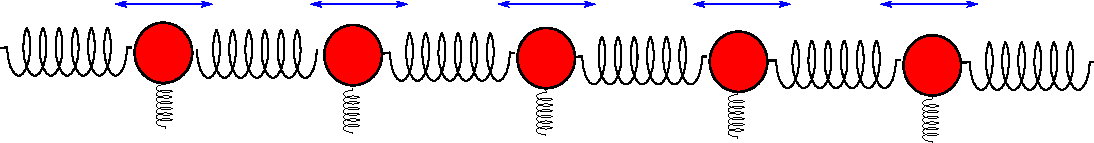
\includegraphics[width=8cm]{oscillator.pdf}
  \caption{}
  \label{fig:oscillator}
\end{figure}


物体間をつなぐバネのバネ定数を$r$、地面と物体をつないでいるバネのバネ定数を$\ell$とすると作用は、
\begin{align}
  S=\int dt L(\phi,\dot{\phi}),\qquad
  L(\phi,\dot{\phi})=\sum_{n=1}^{N}\qty(
    \frac12 m \dot{\phi}_n^2-\frac12 r (\phi_n-\phi_{n-1})^2
    -\frac12 \ell \phi_n^2
  )\label{oscillatorLagrangian}
\end{align}
となります。Lagrangianの中の和の中で$n=1$のとき$\phi_0$が出てきますが、これは周期境界条件
\eqref{periodicboundarycondition}から$\phi_N$と同じです。

ここから基準モードに分けると、単に多数の調和振動子になり、問題が解けるということも力学2の授業でやったと思います。これも後でやります。

物体間の距離を小さくしていく極限で、この系は連続的な波動を記述する系になります。物体間の距離を$a$として$a\to 0$の極限を考えます。ただし、
\begin{align}
  aN=:L,\quad \frac{m}{a}=:\rho,\quad ar=:c^2\rho,\quad \frac{\ell}{a}=:M^2c^4 \rho \label{classicalcontinuum}
\end{align}
を有限に保ったまま$a\to 0$の極限をとります。ラベルを$x:=an$とし、力学変数の書き方を少し変えて$\phi(x,t)$と書きます。$\phi_n(t)$との関係は
\begin{align}
  \phi(x=an,t)=\sqrt{\rho}\phi_n(t)
\end{align}
とします。そうすると周期境界条件\eqref{periodicboundarycondition}は
\begin{align}
  \phi(x=0,t)=\phi(x=L,t)
\end{align}
となり、また\eqref{oscillatorLagrangian}は
\begin{align}
  L=\sum_{n=1}^{N}a\qty[
    \frac12 \rho \dot{\phi}_n^2-\frac12 c^2\rho\qty(\frac{\phi_{n}-\phi_{n-1}}{a})^2-\frac12 M^2c^4 \rho \phi_n^2
  ]
\end{align}
となります。ここで$a\to 0$をとることを考えると、和のところは
\begin{align}
  \sum_{n=1}^{N}a\to\int_{0}^{L}dx
\end{align}
と積分で表示できます。また、$[]$の中の第2項めの$()$の中は
\begin{align}
  \frac{\phi_n-\phi_{n-1}}{a}=\frac{1}{\sqrt{\rho}}\pdv{x}\phi
\end{align}
と微分でかけます。したがって、この極限でLagrangianは、
\begin{align}
  L=\int dx \Lcal,\quad 
  \Lcal=
    \frac12 \dot{\phi}^2-\frac12 c^2 \phi'^2-\frac12 M^2 c^4 \phi^2
\end{align}
となります。積分範囲は省略しました。また$\phi':=\pdv{x}\phi$です。$\Lcal$は、積分してLangrangianになる量ですから\strong{Lagrangian密度}と呼ばれます。これを使うと作用は
\begin{align}
  S=\int d^2x \Lcal
  \quad \int d^2x :=\int dt dx,\qquad
  \Lcal=\frac12 \dot{\phi}^2-\frac12 c^2 \phi'^2-\frac12 M^2c^4 \phi^2\label{continuumaction}
\end{align}
と書けます。

さて作用\eqref{continuumaction}で表される理論について詳しく見てみるために、まず運動方程式を求めてみましょう。作用を停留値にさせるような関数$\phi(x,t)$が運動方程式になるのでした。停留値とは、$\phi(x,t)$を少しだけずらして$\phi(x,t)+\delta \phi(x,t)$にしても作用の値が変わらないようになることです。実際\eqref{continuumaction}で作用の変分を計算してみると
\begin{align}
  \delta S
  =\int d^2x( \dot{\phi}\delta\dot{\phi}-c^2\phi'\delta \phi'-M^2c^4\phi\delta \phi)
  =\int d^2x\delta \phi( -\ddot{\phi}+c^2\phi''-M^2c^4\phi)
\end{align}
となります。最後の変形では部分積分をしました。境界条件は表面項が消えるようにとっています。$\delta \phi$は任意の微小な変分ですから、$\delta S=0$から
\begin{align}
  \ddot{\phi}-c^2\phi''+M^2c^4\phi=0
  \label{eomKG2}
\end{align}
という方程式を得ます。これは、$M=0$のときは波動方程式になるというのは力学2の授業で習ったと思います。

さて、\eqref{eomKG2}で$c$を光速と思ってみると2次元のKlein-Gordon方程式になります。ですからこの理論にはLorentz対称性があります。これは、作用\eqref{continuumaction}がLorentz変換で不変であることからも言えます。後から見るように、この系を量子化すると「粒子」が現れ、状態によって粒子の数は様々です。連続極限をとる前の系はなんの変哲もない連成振動の系ですから、量子化したときに負の確率が現れたり、エネルギー固有値の下限がなくなったりというような病的なことは起こりません。つまり、Lorentz対称性をもち、数が変化する粒子を記述することができるわけです。これを素粒子を記述するのに用いるというのが場の理論のアイデアです。

ここで、少しだけ注意を述べます。\eqref{oscillatorLagrangian}の作用で表される系を量子化するのには何の困難もありません。実際に欲しいのは連続理論ですから、量子論で連続極限をとる必要があります。この連続極限には実際には微妙さがあります。場の理論の発散の問題について聞いたことがある人もいるかと思います。この連続極限をとる際に、うまくやらないと物理量が無限になってしまうことがあります。「極限」をとるのですから、うまくやらないと発散するのは当然ですね。しかし多くの場の理論の教科書では、連続理論の作用\eqref{continuumaction}から始めて量子化するという手続きをとっています。これは本当は微妙な手続きなのですが、ある程度のところまでは深く考えなくてもうまくいってしまいます。そして、あるときに突然発散が出てきて驚く、ということになります。

この講義では、実用的な計算手法を学ぶというよりは、場の理論についての正しいイメージを持ってもらうために、普通の場の理論の教科書ではとばされている\eqref{oscillatorLagrangian}の量子化から始めたいと思います。そこから連続極限をとるという正しい手続きをとって、どういう発散が出るのか、それをどう処理するのかということを簡単に説明したいと思います。

\section{量子化と粒子}
\label{sec:discretequantization}
では、\eqref{oscillatorLagrangian}の系の量子化をやっていきます。ここでは、特に新しいことをやっていないことに注意してください。

まずは、正準形式に直します。$\phi_n$に正準共役な運動量を$\pi_n$とすると
\begin{align}
  \pi_n=\pdv{L}{\dot{\phi}_n}=m\dot{\phi}_n
\end{align}
という関係があります。Hamiltonianは
\begin{align}
  H=\sum_{n}\pi_n \dot{\phi}_n-L=\sum_{n}\frac{1}{2m}\pi_n^2+V(\phi),\quad 
  V(\phi):=\sum_n\qty(\frac12 r (\phi_n-\phi_{n-1})^2
  +\frac12 \ell \phi_n^2
  )
\end{align}
となります。$n$の和は省略していますが、$1$から$N$までです。

さて、これを量子化しましょう。量子化とは、$\phi_n,\ \pi_n$などを演算子にすることでした。ちゃんと演算子にしたことを強調するために、しばらくは演算子を$\phih_n,\pih_n$と書くことにします\footnote{慣れてくると記号をだんだん区別しなくなります。教科書などを読むときには注意してください。}。これらの演算子は正準交換関係
\begin{align}
  [\phih_m,\pih_n]=i\hbar\delta_{mn},\quad
  [\phih_m,\phih_n]=[\pih_m,\pih_n]=0\label{canonicalcommutationrelation}
\end{align}
を満たします。新しいことをやっていないことを強調するために、この章では$\hbar$をあらわに書くことにします。Hamiltonianも演算子になり
\begin{align}
  \Hh=\sum_{n}\frac{1}{2m}\pih_n^2+V(\phih)
\end{align}
となります。一般に量子化のときには、演算子順序の問題があるのですが、今の場合素朴な置き換えを行ったとき、各項で掛け算されている演算子が可換なので、今のような素朴な置き換えでいくことにします。

さて、Heisenberg描像で時間発展を調べることにしましょう\footnote{みなさんはきっとSchrödinger描像の方が慣れているので、なぜSchrödinger描像で考えないのかと思うかもしれません。理由はHeisenberg描像の方がLorentz不変性が比較的見やすいからです。しかし、Schrödinger描像でScrödinger方程式を書いてみて解析するというのは、非常に良い練習問題だと思いますので、興味ある人はぜひ挑戦してみてください。}。Heisenberg方程式は
\begin{align}
  \dot{\phih}_n=\frac{i}{\hbar}[\Hh,\phih_n]=\frac{1}{m}\pih_n,\\
  \dot{\pih}_n=\frac{i}{\hbar}[\Hh,\pih_n]=-(2r+\ell)\phih_n+r \phih_{n-1}+r\phih_{n+1}
\end{align}
となります。これらから
\begin{align}
  m\ddot{\phih}_n=\frac{i}{\hbar}[\Hh,\pih_n]=-(2r+\ell)\phih_n+r \phih_{n-1}+r\phih_{n+1}\label{oscillatoreom}
\end{align}
という式を得ます。これは、古典的な運動方程式で$\phi_n$を形式的に演算子$\phih_n$に置き換えたものと同じですね。実は、この後の方程式を解くところも形式的に同じです。

さて、方程式\eqref{oscillatoreom}は古典論の場合と同じように、基準モードに展開することで解けます。今の場合は基準モードに展開するのは離散的なFourier変換をするのと同じです。つまり
\begin{align}
  \phih_n(t)=\sum_{u=N_{-}}^{N_{+}}e^{\frac{2\pi i u n}{N}}\chih_{u}(t)\label{modeexpansion}
\end{align}
となるように$\chih_{u}(t)$を導入します。ここで、$N_{\pm}$は、
\begin{align}
  &N_{-}=-\frac{N-1}{2},\ N_{+}=\frac{N+1}{2}\qquad &(N \text{が奇数}),\\ 
  &N_{-}=-\frac{N}{2},\ N_{+}=\frac{N}{2}+1\qquad &(N \text{偶数})
\end{align}
としています。これは単に整数$u$に対して$\chih_u(t)$が$\chih_{u+N}(t)=\chih_{u}(t)$を満たすので、代表元をどう取るかを指定しているだけです。$u=1,\dots, N$でも良いのですが、後で連続極限を取るときの都合上、だいたい$0$を真ん中にして左右で同じくらいになるようにしています。今後$u$の和の範囲を省略したら$N_{-}$から$N_{+}$までの和ということにします。\eqref{modeexpansion}を\eqref{oscillatoreom}に代入し整理すると
\begin{align}
  m\ddot{\chih}_{u}=-m\omega_{u}^2\chih_{u},\quad
  \omega_{u}:=\frac{1}{\sqrt{m}}\sqrt{\ell+4r\sin^2\frac{\pi u}{N}}\label{modeeom}
\end{align}
となり、独立した$N$個の調和振動子になります。調和振動子を生成消滅演算子で解く方法は、皆さん量子力学の授業で習ったと思います。ここでも生成消滅演算子を用いた形にします。

さて、\eqref{modeeom}は調和振動子ですから簡単に解けます。$\Ah_u,\ \Bh_u$を時間によらない演算子として、一般解は
\begin{align}
  \chih_{u}(t)=\Ah_{u}e^{-i\omega_u t}+\Bh_{u}e^{i\omega_u t}
\end{align}
となります。これを\eqref{modeexpansion}に代入すると
\begin{align}
  \phih_{n}(t)=\sum_{u}e^{\frac{2\pi i u n}{N}}
  (\Ah_{u}e^{-i\omega_u t}+\Bh_{u}e^{i\omega_u t})\label{tempmodeex}
\end{align}
となります。ところで、古典的には$\phi_n$は実数でしたから、量子論的には、$\phih_n$はエルミート演算子とすべきです。つまり$\phi_n(t)^{\dag}=\phi_n(t)$です。ここから
\begin{align}
  \sum_{u}e^{\frac{2\pi i u n}{N}}
  (\Ah_{u}e^{-i\omega_u t}+\Bh_{u}e^{i\omega_u t})
  &=\sum_{u}e^{\frac{-2\pi i u n}{N}}
  (\Ah_{u}^{\dag}e^{i\omega_u t}+\Bh_{u}^{\dag}e^{-i\omega_u t})\nonumber\\
  &=\sum_{u}e^{\frac{2\pi i u n}{N}}(\Ah_{-u}^{\dag}e^{i\omega_u t}+\Bh_{-u}^{\dag}e^{-i\omega_u t})
\end{align}
という条件を得ます。1行目から2行目への変換では、$u$を$-u$と書きました。また$\omega_{u}=\omega_{-u}$という関係を使っています。ここから両辺逆変換し、任意の$t$で成り立つことを用いると
\begin{align}
  \Ah_{u}^{\dag}=\Bh_{-u}
\end{align}
という関係式を得ます。これを\eqref{tempmodeex}に代入して変形していきます。
\begin{align}
  \phih_{n}(t)
  =\sum_{u}e^{\frac{2\pi i u n}{N}}\Ah_{u}e^{-i\omega_u t}+\sum_{u}e^{\frac{2\pi i u n}{N}}\Bh_{u}e^{i\omega_u t}\nonumber\\
  =\sum_{u}e^{\frac{2\pi i u n}{N}}\Ah_{u}e^{-i\omega_u t}+\sum_{u}e^{\frac{2\pi i u n}{N}}\Ah_{-u}^{\dag}e^{i\omega_u t}\nonumber\\
  =\sum_{u}e^{\frac{2\pi i u n}{N}}\Ah_{u}e^{-i\omega_u t}+\sum_{u}e^{\frac{-2\pi i u n}{N}}\Ah_{u}^{\dag}e^{i\omega_u t}\nonumber\\
  =\sum_{u}(\Ah_{u}e^{-i(\omega_u t-k_u x_n)}+\Ah_{u}^{\dag}e^{i(\omega_u t-k_u x_n)}).\label{tempmodeex2}
\end{align}
2行目から3行目に行くときに、2項目だけ$u\to -u$の変換を行いました。最後の行では、雰囲気を出すために
\begin{align}
  k_u:=\frac{2\pi u}{Na},\quad x_n:=na
\end{align}
という記号を導入しました。$a$はバネで繋がれた2つの物体の釣り合いの位置の間隔です。つまり、$x$はラベル$n$の物体の釣り合いの位置の座標です。最後の表式では、$u>0$の場合が右回り(x軸正の方向に進む)モード、$u<0$の場合が左回り(x軸負の方向に進む)モード、であることがあらわに見て取れます。

ここで出てきた$\Ah_u,\Ah_u^{\dag}$がだいたい生成消滅演算子です。ただし皆さんが習ったものとは、規格化が異なります。これを見ていきましょう。
正準交換関係\eqref{canonicalcommutationrelation}を用いるために、まず$\Ah_u,\ \Ah_u^{\dag}$を$\phih_n,\pih_n$で表すことを考えます。Heisenberg方程式の片方から$\pih_n(t)=m\dot{\phih}_n(t)$でしたから、\eqref{tempmodeex2}より
\begin{align}
  \pih_n(t)=m\sum_{u}(-i\omega_{u}\Ah_{u}e^{-i(\omega_u t-k_u x_n)}+i\omega_u\Ah_{u}e^{i(\omega_u t-k_u x_n)})
\end{align}
を得ます。ここから$\Ah_u,\ \Ah_u^{\dag}$について解くわけですが、これらは時間$t$によらないので式の簡単のために$t=0$として考えます。いつものように$t=0$のときの演算子を引数を省略して書くと
\begin{align}
  &\phih_n=\sum_{u}(\Ah_{u}+\Ah_{-u}^{\dag})e^{ik_u x_n},\\
  &\pih_n=m\sum_{u}(-i\omega_{u}\Ah_{u}+i\omega_u\Ah_{-u})e^{ik_u x_n}\label{tempmodeex3}
\end{align}
となります。両方の式とも、第2項目は$u\to -u$の変換を行っています。これを逆に解くには、両辺に$e^{-ik_{u'}x_n}$をかけて$n$について和をとるということをします。その際に便利な公式は$-N<u<N$の場合に
\begin{align}
  \sum_{n}e^{\frac{2\pi i u n}{N}}=N\delta_{u,0}
\end{align}
という式が成り立つことです。そうすると\eqref{tempmodeex3}から
\begin{align}
  N(\Ah_u+\Ah_{-u}^{\dag}) =\sum_{n}\phih_n e^{-ik_u x_n},\nonumber\\
  -iN\omega_{u}m(\Ah_u-\Ah_{-u}^{\dag})  =\sum_{n}\pih_n e^{-ik_u x_n}
\end{align}
という式を得ます。これらから
\begin{align}
  \Ah_u&=\frac{1}{2N}\sum_{n}(\phih_n+\frac{i}{\omega_u m}\pih_n)e^{-ik_ux_n}\nonumber\\
  \Ah_u^{\dag}&=\frac{1}{2N}\sum_{n}(\phih_n-\frac{i}{\omega_u m}\pih_n)e^{ik_ux_n}\label{tempmodeex4}
\end{align}
という表式を得ます。

さて、\eqref{tempmodeex4}から、$\Ah_u,\Ah_u^{\dag}$を含む交換関係を計算しましょう。
\begin{align}
[\Ah_u,\Ah_{u'}]
&=\frac{1}{4N^2}\sum_{n,n'}e^{-ik_ux_n-ik_{u'}x_{n'}}[\phih_n+\frac{i}{\omega_{u}m}\pih_n,\phih_{n'}+\frac{i}{\omega_{u'}m}\pih_{n'}]\nonumber\\
&=\frac{1}{4N^2}\sum_{n,n'}e^{-ik_ux_n-ik_{u'}x_{n'}}i\hbar\delta_{n,n'}\qty(\frac{i}{\omega_{u'}m}-\frac{i}{\omega_{u}m})\nonumber\\
&=\frac{1}{4N^2}\sum_{n}e^{-ik_ux_n-ik_{u'}x_{n}}i\hbar\qty(\frac{i}{\omega_{u'}m}-\frac{i}{\omega_{u}m})\nonumber\\
&=\frac{1}{4N}\delta_{u,-u'}i\hbar\qty(\frac{i}{\omega_{u'}m}-\frac{i}{\omega_{u}m})\nonumber\\
&=0
\end{align}
同様にして$[\Ah_u^{\dag},\Ah_{u'}^{\dag}]=0$です。$[\Ah_u,\Ah_{u'}^{\dag}]$も同様の方針で計算すると
\begin{align}
  [\Ah_u,\Ah_{u'}^{\dag}]=\frac{\hbar}{2N\omega_{u}m}\delta_{u,u'}
\end{align}
という結果を得ます。ですから
\begin{align}
  \ah_{u}=\sqrt{\frac{2N\omega_um}{\hbar}}\Ah_{u}
\end{align}
を導入すると
\begin{align}
  [\ah_u,\ah_{u'}]=[\ah_u^{\dag},\ah_{u'}^{\dag}]=0,\qquad
  [\ah_u,\ah_{u'}^{\dag}]=\delta_{u,u'}
\end{align}
となり、量子力学の授業で出てきた生成消滅演算子と同じ規格化になります。これを用いてHeisenberg演算子を表すと
\begin{important}
  \begin{align}
    \phih_n(t)&=\sum_{u}\sqrt{\frac{\hbar}{2N\omega_um}}
    (\ah_ue^{-i(\omega_u t -k_ux_n)}
    +\ah_u^{\dag}e^{i(\omega_u t -k_ux_n)})\label{discretefield}\\
    \pih_n(t)&=\sum_{u}\sqrt{\frac{\hbar}{2N\omega_um}}
    (-im\omega_{u})
    (\ah_ue^{-i(\omega_u t -k_ux_n)}
    -\ah_u^{\dag}e^{i(\omega_u t -k_ux_n)})\label{discretemomentum}
  \end{align}
\end{important}
となります。

さて、Hamiltonianを見てみましょう。今モード展開によって、系が調和振動子がたくさん集まったものであることはすでに見ました。したがってHamiltonianもたくさんの調和振動子のHamiltonianの和になっているはずです。これを確かめてみましょう。\eqref{modeexpansion}で導入した$\chih_u(t)$を考えるのが便利です。生成消滅演算子で書くと
\begin{align}
  \chih_u(t)=\sqrt{\frac{\hbar}{2N\omega_um}}(\ah_ue^{-i\omega_u t}
  +\ah_{-u}^{\dag}e^{i\omega_u t})
\end{align}
となります。これを用いると
\begin{align}
  \pih_n(t)=\sum_{u}m\dot{\chih}_u(t)e^{ik_ux_n}\label{modeexpansionpi}
\end{align}
となります。Hamiltonianは保存するので、時刻$t=0$で考えればよいのです。そのときの演算子を求めておきます。
\begin{align}
  \chih_u=\sqrt{\frac{\hbar}{2N\omega_um}}(\ah_u
  +\ah_{-u}^{\dag}),\quad
  \dot{\chih}_u=-i\omega_{u}\sqrt{\frac{\hbar}{2N\omega_um}}(\ah_u
  -\ah_{-u}^{\dag}).\label{tempmodeex5}
\end{align}
まず、\eqref{modeexpansion}、\eqref{modeexpansionpi}を用いてHamiltonianを変形していきます。
\begin{align}
  \Hh&=\sum_{n}\frac{1}{2m}\pih_n^2+V(\phih)
  =\sum_{n}\qty(
    \frac{1}{2m}\pih_n^2+\frac12(\phih_n-\phih_{n-1})^2
    +\frac12\ell \phih_n^2
  )\nonumber\\
  &=\sum_n\sum_{u,u'}e^{ik_ux_n+ik_{u'}x_n}\qty(
    \frac{1}{2m}m^2\dot{\chih}_u\dot{\chih}_{u'}
    +\frac12 r (1-e^{-ik_ua})(1-e^{-ik_{u'}a})\chih_u\chih_{u'}
    +\frac12\ell \chih_u\chih_{u'}
  )\nonumber\\
  &=\sum_{u}N\qty(
    \frac{1}{2m}m^2\dot{\chih}_u\dot{\chih}_{-u}
    +\frac12 r (1-e^{-ik_ua})(1-e^{ik_{u}a})\chih_u\chih_{-u}
    +\frac12\ell \chih_u\chih_{-u}
  )\nonumber\\
  &=\sum_{u}N\qty(
    \frac{1}{2m}m^2\dot{\chih}_u\dot{\chih}_{-u}
    +\frac12 m\omega_{u}^2 \chih_u\chih_{-u}
  )
\end{align}
となります。ここでさらに\eqref{tempmodeex5}を代入して整理していきます。
\begin{align}
  \Hh
  &=\sum_{u}N\frac{\hbar}{2N\omega_{u}}\qty(
    -\frac12 \omega_{u}^2(\ah_u-\ah_{-u}^{\dag})(\ah_{-u}-\ah_{u}^{\dag})
    +\frac12 \omega_{u}^2(\ah_u+\ah_{-u}^{\dag})(\ah_{-u}+\ah_{u}^{\dag})
  )\nonumber\\
  &=\sum_{u}\frac12 \hbar\omega_{u}(\ah_{u}\ah_{u}^{\dag}+\ah_{-u}^{\dag}\ah_{-u})=\sum_{u}\frac12 \hbar\omega_{u}(\ah_{u}\ah_{u}^{\dag}+\ah_{u}^{\dag}\ah_{u})\nonumber\\
  &=\sum_{u}\hbar\omega_{u}(\ah_{u}^{\dag}\ah_{u}+\frac12)
\end{align}
となって、予想通りたくさんの調和振動子のHamiltonianの和になりました。量子力学の授業でやったようにモード$u$にいる「粒子数」の演算子$\Nh_u:=\ah_u^{\dag}\ah_u$を導入すると
\begin{important}
\begin{align}
    \Hh = \sum_{u}\hbar
    \omega_{u}\Nh_{u}
    +\sum_{u}\frac12 \hbar\omega_{u}\label{oscillatorhamiltonian}
\end{align}
\end{important}
を得ます。

ここまで来れば、もう問題は解けています。量子力学の授業でやったように基底状態$\ket{0}$は、すべての$u$に対して
\begin{align}
  \ah_u\ket{0}=0
\end{align}
となる状態です。場の理論の文脈では、この状態は粒子が1つもない状態ですから\strong{真空}と呼ばれます。真空のエネルギーを求めてみると
\begin{align}
  \Hh\ket{0}=E_0\ket{0},\quad E_0=\sum_{u}\frac12 \hbar\omega_{u}
\end{align}
となります。これは、たくさんの調和振動子の基底状態のエネルギーを合わせたものです。今の場合は、$E_0$は有限の定数になりますので、何の問題もありません。

励起状態は真空$\ket{0}$に$\ah_{u}^{\dag}$をかけることにより作れます。このような励起状態を粒子がある状態と思う、というのがミソです。例えば
\begin{align}
  \ah_{u}^{\dag}\ket{0}
\end{align}
という状態は、波数$k_u$をもつ1粒子状態と思うことができます。そのエネルギーは真空に比べて$\hbar \omega_u$だけ大きくなるので、これを粒子のエネルギーと思うことができます。高校のときか、大学の1年生か2年生のときに「角振動数$\omega$の波は粒子描像があって、1つの粒子のエネルギーは$\hbar\omega$である」という話を聞いたことがあるのではないでしょうか。今、まさにそれを導出しました。さらに
\begin{align}
  \ah_{u}^{\dag}\ah_{u'}^{\dag}\ket{0}
\end{align}
は2粒子状態と思うことができます。$u$と$u'$を入れ替えても状態ベクトルに符号は出ませんから、この粒子は\strong{ボゾン}であることが分かります。さらに、この状態のエネルギーと真空のエネルギーとの差は、それぞれの粒子のエネルギー$\hbar\omega_u,\hbar\omega_{u'}$の単なる和になります。これは、この2粒子の間に相互作用が無いということです。つまり、今の系は自由な粒子を記述するので場の理論の文脈では「自由場の理論」と呼ばれます。

今の系で$\ell=0$として、さらに3次元的にしたものは、固体の格子振動を記述する良い模型です。口語的に言えば固体中を伝わる「音」のモデルです。そのときに出てくる粒子は\strong{フォノン}(phonon)と呼ばれます。フォノンとは「音の粒子」という意味です。

この講義の目的は、相対論的な粒子をあつかうことです。そのためには、連続極限を考えなければなりません。次の節では、連続極限を考え、これが相対論的な粒子を記述していることを見ます。

\section{連続極限}
\subsection{真空のエネルギー}
連続極限を考えます。素朴には\eqref{classicalcontinuum}のような量を有限に保って、$a\to 0$とすれば良いでしょう。これをやってみようとすると、次のような問題が発生します。\eqref{oscillatorhamiltonian}の真空のエネルギーの部分
\begin{align}
  E_0=\sum_{u}\frac12 \hbar \omega_{u}
\end{align}
が発散してしまいます。これについて少し考察してみましょう。

1つめの解決策は、$E_0$は観測量に現れないので気にしないというものです。Heisenberg描像では、Hamiltonian $\Hh$ はHeisenberg方程式に交換関係の形でのみ現れます。ですからc数のものが足し算してあったとしても、Heisenberg方程式からは消えてしまいます。Schrödinger描像でも、$E_0$はすべての状態に共通の位相としてのみ現れるので、期待値には出てきません。したがって、Hamiltonianから$E_0$を黙って引いて
\begin{align}
  \Hh=\sum_{u}\hbar \omega_{u}\Nh_{u}
\end{align}
とします。\footnote{この1つめの解決策には少しだけ心配なことがあります。重力がある場合、$E_0$は宇宙項として観測されてしまうのです。}

2つめの解決策は、現代での標準的な考え方です。そもそもLagrangian\eqref{oscillatorLagrangian}を書く段階で、エネルギーの基準を全く気にしていませんでした。それが悪かったのです。最初から、パラメータ$\Omega$として定数のポテンシャルエネルギーを入れて
\begin{align}
  L(\phi,\dot{\phi})=\sum_{n=1}^{N}\qty(
    \frac12 m \dot{\phi}_n^2-\frac12 r (\phi_n-\phi_{n-1})
    -\frac12 \ell \phi_n^2-\Omega
  )
\end{align}
としておきます。そうするとHamiltonianは
\begin{align}
  \Hh=\sum_{u}\hbar \omega_{u}\Nh_{u}+\sum_{u}\frac12 \hbar \omega_{u}+N\Omega
\end{align}
となります。連続極限をとるときには\eqref{classicalcontinuum}とともに
\begin{align}
  E_0=\sum_{u}\frac12\hbar\omega_{u}+N\Omega
\end{align}
を固定して$a\to 0$にします。この2つめの解決策のような手法を「繰り込み」と呼びます。今の場合は、真空のエネルギーについて考えましたが、相互作用のある場の理論では、他のパラメーターの繰り込みも考える必要があります。繰り込みについての詳しいことは、M1の場の理論の授業などで習います。

\subsection{連続極限での場}
次に連続極限で場がどうなるか考えてみましょう。古典論と同様にして考えることにします。
\begin{align}
  \phih(x,t):=\sqrt{\rho}\phih_{n}(t)\qquad (x=na,\ L=Na,\ \rho=\frac{m}{a})
\end{align}
と定義します。これに\eqref{discretefield}の表式を代入して
\begin{align}
  \phih(x,t)=\sum_{u=-\infty}^{\infty}\sqrt{\frac{\hbar}{2L\omega_{u}}}(\ah_{u}e^{-i(\omega_ut-k_ux)}
  +\ah^{\dag}_{u}e^{i(\omega_ut-k_ux)})
\end{align}
という表式を得ます。ここで
\begin{align}
  k_u=\frac{2\pi u}{L},\quad \omega_{u}=\frac{1}{\hbar}\sqrt{M^2c^4+(\hbar k_u)^2c^2},\quad \frac{M^2c^4}{\hbar^2}\rho=\frac{\ell}{a}
\end{align}
としました。$\hbar$をあらわに書いたので、$M$の表式が\eqref{classicalcontinuum}と少し変わっています。$c$を光速と思うなら、1粒子のエネルギー$\hbar \omega_{u}$と運動量$\hbar k_u$の関係が、相対論的なものになっていることが分かると思います。

正準運動量の方は、次のように連続的なものを定義します。
\begin{align}
  \pih(x,t):=\frac{1}{\sqrt{\rho}a}\pih_{n}(t).
\end{align}
こうすると、正準交換関係が
\begin{align}
  [\phih(x,t),\pih(x',t)]=[\sqrt{\rho}\phi_{n}(t),\frac{1}{a\sqrt{\rho}}\pih_{n'}(t)]=\frac{ih}{a}\delta_{n,n'}
  \label{tempcommutationrelationcontinuum}
\end{align}
となります。ここで、最後の$\frac{1}{a}\delta_{n,n'}$について考えてみましょう。$x=na,\ x'=n'a$ですから$a\to 0$の極限で
\begin{align}
  \frac{1}{a}\delta_{n,n'}\to
  \begin{cases}
    \infty & (x=x')\\
    0 & (x\ne x')
  \end{cases}
\end{align}
です。さらに
\begin{align}
  \sum_{n}a \frac{1}{a}\delta_{n,n'}=1
\end{align}
という関係と$a\to 0$で
\begin{align}
  \sum_{n=-\infty}^{\infty}a\to \int dx
\end{align}
ということを考え合わせると$a\to 0$で
\begin{align}
  \frac{1}{a}\delta_{n,n'}\to \delta(x-x')
\end{align}
となることが分かります。したがって式\eqref{tempcommutationrelationcontinuum}で連続極限をとると
\begin{important}
  \begin{align}
    [\phih(x,t),\pih(x',t)]=i\hbar\delta(x-x')
  \end{align}
\end{important}
という正準交換関係が得られます。

ここまでで、長さが$L$の円周を空間とする連続的な場の理論が出来ました。結果をまとめておきます。
\begin{important}
  \begin{align}
    \phih(x,t)=\sum_{u=-\infty}^{\infty}\sqrt{\frac{\hbar}{2L\omega_{u}}}(\ah_{u}e^{-i(\omega_ut-k_ux)}
    +\ah^{\dag}_{u}e^{i(\omega_ut-k_ux)}),
  \end{align}
  \begin{align}
    \Hh=\sum_{u=-\infty}^{\infty}\hbar \omega_{u}\ah_{u}^{\dag}\ah_{u}+E_0,
  \end{align}
  \begin{align}
    [\ah_{u},\ah_{u'}^{\dag}]=\delta_{u,u'},
  \end{align}
  \begin{align}
    k_u=\frac{2\pi u}{L},\qquad \omega_{u}=\frac{1}{\hbar}
    \sqrt{M^2c^4+(\hbar k_u)^2c^2}.
  \end{align}
\end{important}

\subsection{無限体積極限}
ここまででは、空間が長さ$L$の円周です。$L\to \infty$の極限をとることを考えましょう。この極限では、運動量$k$も連続的になります。$k_u=\frac{2\pi u}{L}$であったことを思い出すと、$L\to\infty$の極限で
\begin{align}
  \sum_{u=-\infty}^{\infty}\frac{2\pi}{L}\to \int dk
\end{align}
と積分になることが分かります。また生成消滅演算子を
\begin{align}
  \ah(k):=\sqrt{\frac{L}{2\pi}}\ah_{u}
\end{align}
と定義すると交換関係は
\begin{align}
  [\ah(k),\ah(k')^{\dag}]=\frac{L}{2\pi}\delta_{u,u'}\to \delta(k-k')
\end{align}
となります。

これらをまとめておきます。
\begin{important}
  \begin{align}
    \phih(x,t)=\int\frac{dk}{\sqrt{2\pi}}\sqrt{\frac{\hbar}{2\omega_k}}(\ah(k)e^{-i(\omega_{k}t-kx)} + \ah(k)^{\dag}e^{i(\omega_kt-kx)}),
  \end{align}
  \begin{align}
    \Hh=\int dk \hbar \omega_{k}\ah(k)^{\dag}\ah(k),
  \end{align}
  \begin{align}
    \omega_{k}=\frac{1}{\hbar}\sqrt{M^2c^4+(\hbar k)^2c^2}.
  \end{align}
\end{important}
これを見るとちゃんとこの系が相対論的な粒子を記述していることが分かります。

ここでは、\strong{波動を量子化すると粒子が出てくる}ことを飛躍なしに説明したつもりです。しかし、1つだけ説明を飛ばしたことがあります。それは、ここで$\hbar k$と書いたものが1つの粒子の運動量だということです。運動量とは、空間並進対称性に対する保存量でした。これはNoetherの定理を用いて得ることができます。場の理論でのNoetherの定理をちゃんと説明する時間がないので、結果だけ書くと、運動量の演算子$\Ph$は
\begin{align}
  \Ph=\int dk \,\hbar k \ah(k)^{\dag}\ah(k)
\end{align}
となります。ここから
\begin{align}
  [\Ph,\ah(k)^{\dag}]=\hbar k\ah(k)^{\dag}
\end{align}
という交換関係が導かれ、$\ah(k)^{\dag}$で生成される粒子が持つ運動量が$\hbar k$であることが分かります。特に1粒子状態に対して
\begin{align}
  \Ph \ah(k)^{\dag}\ket{0}=\hbar k\ah(k)^{\dag}\ket{0}
\end{align}
が成り立ちます。

\section{この章のまとめ}
この章では、波動を量子化すると粒子が出てくることを説明しました。
\begin{itemize}
  \item 波動のモデルとしてバネでつながったたくさんの物体を考えました。
  \item これを量子化すると粒子が現れました。理論には任意個の粒子を含むことができます。
  \item 連続極限では、真空のエネルギーに発散が現れましたが、繰り込みにより処理できます。
  \item 連続極限、無限体積極限で相対論的な粒子を記述する理論になりました。
\end{itemize}

\chapter{場の理論における作用と正準量子化}
前の章では、連成振動の系の量子論を考えると、粒子が出てくることを見ました。また、連続極限を考えると、$c$を光速とみなすと相対論的な粒子の系の記述になっていることを見ました。

この章では、古典的な連続理論を、連続理論のまま取り扱う方法を説明します。この方法では、計算などが楽になるので良いです。反面、場の理論の微妙な点を覆い隠してしまっているので、発散などが出た場合、改めて考え直す必要があります。

この章から、また4次元時空を考えます。また、$c=\hbar=1$の自然単位系に戻ります。


\section{場の理論の作用}
この講義では、簡単のためにスカラー場が1つだけの理論を考えます。$\phi(x)$をそのスカラー場として、その作用は、
\begin{align}
  S[\phi]=\int d^4x \Lcal(\phi(x),\del\phi(x)),\qquad \int d^4x :=\int dt\int d^3\xb\label{fieldtheoryaction}
\end{align}
とLagrangian密度$\Lcal(\phi,\del\phi)$を用いて書かれているとします。$\Lcal(\phi,\del\phi)$は$\phi,\del_{\mu}\phi\ (\mu=0,1,2,3)$の(汎関数ではなく)関数で、スカラー場であるとします。例えば$V(\phi)$を$\phi$の関数として
\begin{align}
  \Lcal=\frac12\del_{\mu}\phi \del^{\mu}\phi-V(\phi)
\end{align}
というものです。$\Lcal$がスカラー場ですから、その積分である$S$もスカラーです。したがって、あらわなLorentz不変性があります。

しつこいようですが、解析力学でやったこととつなげるために、空間を離散化してみます。$\xb=a\nb,\ \nb=(n_1,n_2,n_3)\in \Zb^3$とし、$\phi(x)=\phi_{\nb}(t)$と書いてみます。空間方向の微分は、$i$方向の単位ベクトル$\eb_i$を用いて$\del_i\phi(x)\to \frac{1}{a}(\phi_{\nb+\eb_i}(t)-\phi_{\nb}(t))$と置き換えるのが適当でしょう。作用は
\begin{align}
  S=\int dt L,\qquad L=\sum_{\nb}a^3 \Lcal(\phi_{\nb}(t),\dot{\phi}_{\nb}(t), \frac{1}{a}(\phi_{\nb+\eb_i}(t)-\phi_{\nb}(t)))
  \label{discreteaction}
\end{align}
とします。こうなれば沢山の物体がある普通の力学系になります。古典論の範囲では、適切に$a\to 0$の極限をとれば\eqref{fieldtheoryaction}に戻ります。

運動方程式は最小作用の原理から出します。これは、$\phi(x)\to \phi(x)+\delta\phi(x)$と任意の微小量$\delta\phi(x)$変化させたとき、作用の変化分$\delta S=S[\phi+\delta \phi]-S[\phi]$が
\begin{align}
  \delta S=0
\end{align}
となるような$\phi$が実際に起こる運動だという原理です。

少し、この変分計算の仕方を簡単に説明します。$\delta$はだいたい微分みたいな感じで作用します。つまり
\begin{align}
  \delta(A+B)=\delta A+\delta B,\quad \delta(AB)=(\delta A)B+A\delta B,\quad
  \delta(aA)=a\delta A\ (a\text{は$\phi$によらないもの})
\end{align}
のような計算が成り立ちます。特に微分や積分は足し算、引き算、$\phi$によらないものをかける、というようなもので出来ていますから
\begin{align}
  \delta(\del_{\mu}A)=\del_{\mu}(\delta A),\delta \int d^4x A=\int d^4x\delta A
\end{align}
などが成り立ちます。また、$V(A)$を$A$の関数とすると
\begin{align}
  \delta V(A)=V(A+\delta A)-V(A)=V'(A)\delta A
\end{align}
となります。同様に$V(A,B)$を$A,B$の関数とすると
\begin{align}
  \delta V(A,B)=\del_{A}V(A,B)\delta A+\del_{B}V(A,B)\delta B
\end{align}
などとなります。

これらを用いて\eqref{fieldtheoryaction}の作用の変分をとってみましょう。
\begin{align}
  \delta S=\int d^4x \delta \Lcal(\phi,\del \phi)
  =\int d^4 x \qty(
    \pdv{\Lcal}{\phi}\delta \phi+\pdv{\Lcal}{(\del_{\mu}\phi)}\delta(\del_{\mu}\phi)
  )\nonumber \\
  =\int d^4 x \delta \phi(x) \qty(
    \pdv{\Lcal}{\phi(x)}-\del_{\mu}\pdv{\Lcal}{(\del_{\mu}\phi(x))}
  )
\end{align}
となります。1行目から2行目へは、部分積分をしました。$\delta \phi(x)$は任意の微小な変分ですから、$\delta S=0$となるためには
\begin{align}
  \pdv{\Lcal}{\phi(x)}-\del_{\mu}\pdv{\Lcal}{(\del_{\mu}\phi(x))}=0
\end{align}
となる必要があります。これが運動方程式です。

\section{場の理論の正準形式}
さて、この系を正準形式で書いていきましょう。まず、大前提として正準形式では時間を特別扱いしますから、明白なLorentz不変性がなくなります\footnote{経路積分形式ですと、明白なLorentz不変性を保ったまま定式化できます。}。もちろん、今の系はLorentz不変ですから明白でないだけで物理はLorentz不変です。

まず、正準運動量を考えます。今の場合、$\xb$はただのラベルですから、気持ち的に正準運動量は
\begin{align}
  \pi(\xb)=\pdv{L}{\dot{\phi}(\xb)}
  \quad \mbox{\Huge ?}
\end{align}
としたい気がします。しかし、これでは$\xb$が連続的であるために記号の意味が分かりません。そこで一旦離散的な場合にもどって考えます。場を$\phi_{\nb}$として式\eqref{discreteaction}の作用を考えます。すると普通に
\begin{align}
  \pi_{\nb}:=\pdv{L}{\dot{\phi}_{\nb}}=a^3\pdv{\Lcal}{\dot{\phi}_{\nb}}
\end{align}
となります。しかし、これで素朴に$a\to 0$の極限をとってしまうと$\pi_{\nb}\to 0$となってしまいます。なので
\begin{align}
  \pi(\xb=a\nb):=\frac{1}{a^3}\pi_{\nb}=\pdv{\Lcal}{\dot{\phi}_{\nb}}
\end{align}
と定義します。すると連続理論にもどって
\begin{align}
  \pi(\xb)=\fdv{L}{(\dot{\phi}(\xb))}=\pdv{\Lcal}{(\dot{\phi}(\xb))}
\end{align}
となります。ここで、汎関数微分$\fdv{L}{(\dot{\phi}(\xb))}$の記号を導入しました。これは、偏微分の添字を連続的にしたようなもので
\begin{align}
  \fdv{L}{(\dot{\phi}(\xb))}=\lim_{a\to 0}\frac{1}{a^3}\pdv{L}{\dot{\phi}_{\nb}}
\end{align}
となるものです。

もう少し汎関数微分について説明します。一般的に$\phi(\xb)$の汎関数$A$に対して、$\phi(\xb)\to \phi(\xb)+\delta \phi(\xb)$としたときに
\begin{align}
  \delta A=\int d^3\xb \delta \phi(\xb)\fdv{A}{\phi(\xb)}
\end{align}
となるとして$\fdv{A}{\phi(\xb)}$を定義します。この定義にしたがうと例えば
\begin{align}
  \delta \phi(\xb')=\int d^3\xb \delta \phi(\xb)\delta^3(\xb-\xb')
\end{align}
ですから
\begin{align}
  \fdv{\phi(\xb')}{\phi(\xb)}=\delta^3(\xb-\xb')
\end{align}
となります。

ここで得た教訓は、場の理論の解析力学をやるには、次のような置き換えをやれば、大体良いということです。
\begin{itemize}
  \item $\xb$は連続的だが、ただのラベル。
  \item 偏微分は汎関数微分に置き換える。
  \item ラベルについての和は、積分に置き換える。
\end{itemize}

これを踏まえてPoisson括弧を考えてみましょう。$A,B$を$\pi(\xb),\phi(\xb)$の汎関数とします。上の処方をPoisson括弧でやると
\begin{align}
  \{A,B\}=\int d^3\xb\qty(
    \fdv{A}{\phi(\xb)}\fdv{B}{\pi(\xb)}
    -\fdv{A}{\pi(\xb)}\fdv{B}{\phi(\xb)}
  )
\end{align}
と定義するのが適当です。ここから例えば
\begin{align}
\{\phi(\xb'),\pi(\xb)\}=\delta^3(\xb-\xb'),\qquad  \{\phi(\xb'),\phi(\xb)\}=\{\pi(\xb'),\pi(\xb)\}=0
\end{align}
という式が得られます。

次にHamiltonianを考えます。上で見た置き換え、あるいは一旦離散的なものを考えてから連続極限をとって考えると
\begin{align}
  H=\int d^3\xb \pi(\xb)\dot{\phi}(\xb)-L=\int d^3\xb \Hcal,\nonumber\\
  \Hcal=\pi(\xb)\dot{\phi}(\xb)-\Lcal
\end{align}
となります。この$\Hcal$は積分してHamiltonianになるので、\strong{Hamiltonian密度}と呼びます。物理的には積分してエネルギーになるので、エネルギー密度です。

例をやってみましょう。
\begin{align}
  \Lcal
  =\frac{1}{2}\del_{\mu}\phi \del^{\mu}\phi-\frac12 m^2 \phi^2
  =\frac{1}{2}\dot{\phi}^2-\frac12 (\bnabla \phi)^2-\frac12 m^2 \phi^2\label{KGLagrangian}
\end{align}
を考えます。ここから導かれる運動方程式はKlein-Gordon方程式になります。正準運動量は
\begin{align}
  \pi(\xb)=\pdv{\Lcal}{\dot{\phi}(\xb)}=\dot{\phi}(\xb)
\end{align}
となります。Hamiltonianは
\begin{align}
  H=\int d^3\xb \Hcal,\qquad \Hcal=\frac12 \pi(\xb)^2+\frac12 (\bnabla \phi)^2+\frac12 m^2 \phi^2
\end{align}
となります。

\section{Klein-Gordon場の量子化}

最後に\eqref{KGLagrangian}で表されるKlein-Gordon場の量子化を考えましょう。既に正準形式を作ってあるので、あとはPoisson括弧を交換子に置きかえるだけです。特に
\begin{align}
  [\phih(\xb),\pih(\xb')]=i\delta(\xb-\xb')
\end{align}
となります。

\ref{sec:discretequantization}節でやったのと同様に解いていきます。Heisenberg方程式はKlein-Gordon方程式になります。
\begin{align}
  \ddot{\phih}(x)-\bnabla^2\phih(x)+ m^2\phih(x)=0.
\end{align}
これはモード展開するとたくさんの独立した調和振動子になります。
今の場合、モード展開はFourier変換です。
\begin{align}
  \phih(t,\xb)=\int\dk \chih(t,\kb)e^{i\kb\cdot\xb}
\end{align}
とすると運動方程式は
\begin{align}
  \ddot{\chih}(t,\kb)=-\omega(\kb)^2 \chih(t,\kb),\qquad
  \omega_{\kb}:=\sqrt{m^2+\kb^2}
\end{align}
と調和振動子になります。

一般解は
\begin{align}
  \chih(t,\kb)=\Ah(\kb)e^{-i\omega(\kb) t}+\Bh(\kb)e^{i\omega(\kb)t}
\end{align}
となります。$\phih(x)$がエルミート演算子であることを考え合わせると
\begin{align}
  \phih(x)=\int \dk (\Ah(\kb)e^{-ik\cdot x} +\Ah(\kb)^{\dag}e^{ik\cdot x})
\end{align}
となります。ここで4元ベクトル$k^{\mu}$を$\kb=(k^1,k^2,k^3),\ k^0=\omega(\kb)$として導入しました。また$k\cdot x=k_{\mu}x^{\mu}$です。

$\Ah(\kb)^{\dag},\Ah(\kb)$が生成消滅演算子になります。これの交換関係を計算しておくと
\begin{align}
  [\Ah(\kb),\Ah(\kb')]=[\Ah(\kb)^{\dag},\Ah(\kb')^{\dag}]=0,\qquad
  [\Ah(\kb),\Ah(\kb)]=\frac{1}{2\omega(\kb)}(2\pi)^3\delta^{3}(\kb-\kb')
\end{align}
となります。ですから
\begin{align}
  \ah(\kb):=\sqrt{\frac{2\omega(\kb)}{(2\pi)^3}}\Ah(\kb)
\end{align}
とすると
\begin{align}
  [\ah(\kb),\ah(\kb)^{\dag}]=\delta^3(\kb-\kb')
\end{align}
となります。

Hamiltonianも同様に計算できます。真空のエネルギーは無限になりますが、これは手で取り除くことにします。この結果をまとめておきます。
\begin{important}
  \begin{align}
    \phih(x)=\int\frac{d^3\kb}{\sqrt{(2\pi)^32\omega(\kb)}}
    (\ah(\kb)e^{-ik\cdot x} +\ah(\kb)^{\dag}e^{ik\cdot x})
  \end{align}
  \begin{align}
    \omega(\kb)=\sqrt{m^2+\kb^2}
  \end{align}
  \begin{align}
    [\ah(\kb),\ah(\kb')]=[\ah(\kb)^{\dag},\ah(\kb')^{\dag}]=0,\qquad
    [\ah(\kb),\ah(\kb')^{\dag}]=\delta^3(\kb-\kb')
  \end{align}
  \begin{align}
    \Hh=\int d^3\kb\omega(\kb)\ah(\kb)^{\dag}\ah(\kb).
  \end{align}
\end{important}
ここから、やはりこの理論には様々な数の粒子を含む理論であることが分かります。また、その粒子のエネルギーと運動量の関係は相対論的であることが分かります。さらに粒子の間に相互作用はなく、自由な粒子になっています。そして、粒子はスピン0でボゾンです。

\section{この先}

ここから先について、少しだけお話しします。

ここまでのところで、場を量子化すると粒子が出てくるということは分かってもらえたと思います。しかし、この粒子は相互作用のない粒子でした。つまり、状態はいくつかの粒子が自由に飛んているだけというものになっています。

粒子同士が互いに力を及ぼすような「相互作用」する物理を記述するためには、理論を少し変形する必要があります。これは、作用が場の2次だけでなく3次以上の項を入れることによって実現されます。例えば$\lambda$を定数として
\begin{align}
  \Lcal=\frac12 \del_{\mu}\phi\del^{\mu}\phi-\frac12 m^2\phi^2-\frac{\lambda}{4!}\phi^4
\end{align}
のようにします。この付け加えた項によって粒子同士の間に相互作用が生まれます。粒子同士の間に力がはたらいたり、時間発展で粒子が出来たり消えたりします。

自由場は完全に解くことができましたが、相互作用のある場の理論は一般的には解けません。したがって、相互作用のある理論で何か計算するためには近似法を用いる必要があります。このうち、最も広く使われている方法が摂動論です。

また、スカラー場$\phi(x)$だけで記述できるのは、スピン0のボゾンでした。ですから、電子や光子を記述するには、別の種類の場を用いる必要があります。
電子は、スピノールの場$\psi(x)$で記述されます。さらに電子はフェルミオンですから、$\psi(x)$は古典的にはGrassmann数という、掛け算が反交換するようなものになります。自由な電子を記述する作用は、
\begin{align}
  S=\int d^4x(\psib(i\gamma^{\mu}\del_{\mu}-m)\psi)
\end{align}
となります。運動方程式が自由なDirac方程式になることは確認できると思います。

また光子は電磁場ですから電磁ポテンシャル$A_{\mu}(x)$で記述されます。光子はボゾンなので、$A_{\mu}(x)$は古典的には交換する場です。この作用は
\begin{align}
  S=\int d^4x \qty(
    -\frac14 F_{\mu\nu}F^{\mu\nu}
  )
\end{align}
となります。

これらを合わせると、電子と光子が相互作用するような理論の作用は
\begin{align}
  S=\int d^4x\qty(
    -\frac14 F_{\mu\nu}F^{\mu\nu}+
    \psib(i\gamma^{\mu}D_{\mu}-m)\psi
  )
\end{align}
となります。この理論は\strong{量子電磁気学}(Quantum Electro-Dynamics, QED)と呼ばれます。物質を表す$\psi$と力を表す$A_{\mu}$が、どちらも場として理論の中にあらわれているのが分かってもらえると思います。

素粒子の標準模型と呼ばれる理論も、何種類かの場を用いて、作用が書けている場の理論です。(ニュートリノの部分を修正した)標準模型は今のところ素粒子のほぼすべての実験結果をよく説明しています。


\appendix
\chapter{特殊相対論でのテンソル算}
\label{app:tensor}
\section{Lorentz変換とEinsteinの規約}
Lorentz変換や、それに伴う様々な物理量の変換を記述するために、次のような記法を導入する。
まず、時空の座標$x^{\mu},\ (\mu=0,1,2,3)$ を
\begin{align}
x^{0}=ct,\quad x^{1}=x,\quad x^{2}=y,\quad x^{3}=z
\end{align}
とする。今後、$x^{\mu}$の$\mu$は上付きの添字であって、べき乗ではないことに注意する。
S系の座標$x^{\mu}$と\Sp 系の座標 $x'^{\mu}$の間が変換の行列成分を$\Lambda^{\mu}{}_{\nu}$とする1次変換
\begin{align}
 x'^{\mu}=\sum_{\nu=0}^{3}\Lambda^{\mu}{}_{\nu}x^{\nu}
\label{lorentz1}
\end{align}
で関係していて、さらに
\begin{align}
s^{2}
:=(x^{0})^{2}-(x^{1})^{2}-(x^{2})^{2}-(x^{3})^{2}
=s'^{2}
:=(x'^{0})^{2}-(x'^{1})^{2}-(x'^{2})^{2}-(x'^{3})^{2}
\end{align}
を満たすとき、この変換を Lorentz 変換と呼ぶのであった。これらの式を簡潔に表すために、まず次の Einstein の規約を導入する。
式\eqref{lorentz1}では、2回出てきている添字$\nu$について和をとっている。今後このような和がたくさん出てくるので、約束として
\emph{1つの項に2回同じ添字が出てきたら、和の記号を書かなくても、その添字が走る範囲で和を取る}ということにする。例えば
\begin{align}
 x'^{\mu}=\Lambda^{\mu}{}_{\nu}x^{\nu}
\label{lorentz2}
\end{align}
は、式\eqref{lorentz1}と全く同じ式である。注意することは、式\eqref{lorentz2}は、式\eqref{lorentz1}と同じであり、$\nu$は
和をとっている添字なので、別の文字にしても、全く同じである。
\begin{align}
\Lambda^{\mu}{}_{\nu}x^{\nu}
=\Lambda^{\mu}{}_{\rho}x^{\rho}
\end{align}
である。このことを利用して\emph{1つの項に同じ添字が3回以上出てこない}ように注意する。

さらに$s^{2}$の表式を簡潔に表すために、次の記号を導入する。
\begin{align}
\eta_{\mu\nu}=\eta^{\mu\nu}
=
\begin{cases}
+1&(\mu=\nu=0),\\
-1&(\mu=\nu=1,2,3),\\
0 &(\mu\ne\nu).
\end{cases}
\end{align}
そうすると$s^{2}$は
\begin{align}
s^{2}=
\eta_{\mu\nu}x^{\mu}x^{\nu}
\end{align}
という簡潔な形に書ける。ここでは、$\mu,\nu$ともに2回ずつ出てきているので、それぞれについて$0,1,2,3$の和をとっていることに
注意する。そうすると、Lorentz変換の条件$s^{2}=s'^{2}$は
\begin{align}
\eta_{\mu\nu}x^{\mu}x^{\nu}
=\eta_{\mu\nu}x'^{\mu}x'^{\nu}
\end{align}
と書ける。右辺の$x'$を\eqref{lorentz2}も用いて$x$で書き換え、先ほどの添字の置き換えの操作を駆使すると
\begin{align}
\eta_{\mu\nu}x^{\mu}x^{\nu}
=\eta_{\rho\sigma}\Lambda^{\rho}{}_{\mu}\Lambda^{\sigma}{}_{\nu}x^{\mu}x^{\nu}
\end{align}
となる。$x^{\mu}$は時空の任意の点なので$x^{\mu}x^{\nu}$の係数を比較して
\begin{important}
\begin{align}
\eta_{\mu\nu}
=\eta_{\rho\sigma}\Lambda^{\rho}{}_{\mu}\Lambda^{\sigma}{}_{\nu}
\label{l3}
\end{align}
\end{important}
を得る。これが変換\eqref{lorentz2}がLorentz変換になるための行列成分$\Lambda^{\mu}{}_{\nu}$に対する条件である。

次に、並進も含めて考えることにする。$b^{\mu}$を4成分ある定数として、S系と\Sp 系が
\begin{align}
x'^{\mu}=\Lambda^{\mu}{}_{\nu}x^{\nu}+b^{\mu}
\end{align}
で結びついている場合を考える。ただし$\Lambda^{\mu}{}_{\nu}$は条件\eqref{l3}を満たすとする。このような変換をPoincare変換と呼ぶ。
このときには、並進があるので、原点からの4次元的距離$s^{2}$は不変ではない。代わりに2つの時空点の座標の差$\Delta x^{\mu}$を用いて作ったこの2点の間の4次元的距離
\begin{align}
\Delta s^{2}=\eta_{\mu\nu}\Delta x^{\mu} \Delta x^{\nu}
\end{align}
が
\begin{align}
\Delta s^{2}=\Delta s'^{2}
\end{align}
を満たす。あるいは、無限小の場合を考えて
\begin{align}
ds^{2}=\eta_{\mu\nu}dx^{\mu}dx^{\nu}
\end{align}
が不変になる。

後のため、次の記号を導入しておく。1つめはクロネッカーのデルタで
\begin{align}
\delta^{\mu}_{\nu}
=
\begin{cases}
1&(\mu=\nu),\\
0 &(\mu\ne\nu).
\end{cases}
\end{align}
これを使うと、上付きの$\eta^{\mu\nu}$と下付きの$\eta_{\mu\nu}$の間には、
\begin{align}
\eta^{\mu\rho}\eta_{\rho\nu}=\delta^{\mu}_{\nu}
\end{align}
の関係があることが分かる。
もう1つは$\Lambda^{\mu}{}_{\nu}$の逆行列$\Lambda^{-1}{}^{\mu}{}_{\nu}$である。つまりこれは
\begin{align}
\Lambda^{\mu}{}_{\rho}\Lambda^{-1}{}^{\rho}{}_{\nu}=\Lambda^{-1}{}^{\mu}{}_{\rho}\Lambda^{\rho}{}_{\nu}=\delta^{\mu}_{\nu}
\end{align}
を満たす。
\section{スカラーとベクトル}
以下、上のPoincare変換を考え、S系から見た量と\Sp 系から見た量を$'$を付けて区別する。

\subsection{スカラー}
1成分の量$f$が、$f=f'$を満たすとき、$f$をスカラーと呼ぶ。例えば、2つの時空点間の4次元的距離の2乗$\Delta s^{2}$、光速$c$などはスカラーである。また、1成分の関数$f(x)$が、$f'(x')=f(x)$のとき、これをスカラー場と呼ぶ。

\subsection{反変ベクトル}
4成分の量$A^{\mu}$が
\begin{important}
\begin{align}
A'^{\mu}=\Lambda^{\mu}{}_{\nu}A^{\nu}
\end{align}
\end{important}
を満たすとき、これを(4元)\emph{反変ベクトル}と呼ぶ。$\Delta x^{\mu}$は反変ベクトルの例である。4成分の関数$A^{\mu}(x)$が、
\begin{important}
\begin{align}
A'^{\mu}(x')=\Lambda^{\mu}{}_{\nu}A^{\nu}(x)
\end{align}
\end{important}
を満たすとき、これを\emph{反変ベクトル場}と呼ぶ。

\subsection{共変ベクトル}
一方、4成分の量$A_{\mu}$が
\begin{important}
\begin{align}
A'_{\mu}\Lambda^{\mu}{}_{\nu}=A_{\nu}
\end{align}
\end{important}
を満たすとき、これを(4元)\emph{共変ベクトル}と呼ぶ。
4成分の関数$A^{\mu}(x)$が、
\begin{important}
\begin{align}
A'_{\mu}(x')\Lambda^{\mu}{}_{\nu}=A_{\nu}(x)
\end{align}
\end{important}
を満たすとき、これを\emph{共変ベクトル場}と呼ぶ。共変ベクトルの1つの重要な例は$A^{\mu}$を反変ベクトルとしたとき、$A_{\mu}:=\eta_{\mu\nu}A^{\nu}$で定義した$A_{\mu}$は共変ベクトルとなることである。これらは逆に、$A^{\mu}=\eta^{\mu\nu}A_{\nu}$とも書ける。このように$\eta_{\mu\nu}$, $\eta^{\mu\nu}$を使って添字を上げ下げし、共変ベクトルと反変ベクトルを行き来することができる。

共変ベクトル場のもう1つの重要な例は、$f(x)$をスカラー場としたとき
\begin{align}
\del_{\mu}f(x):=\frac{\del}{\del x^{\mu}} f(x)
\end{align}
は、共変ベクトル場となることである。別の見方をすると、ナブラの4次元バージョンである微分演算子$\del_{\mu}$は共変ベクトル演算子である。

\subsection{内積}
$A^{\mu}$、$B_{\mu}$をそれぞれ反変ベクトルと共変ベクトルとする。
この2つから作った\emph{$A^{\mu}B_{\mu}$はスカラーになる。}これを$A^{\mu}$と$B_{\mu}$の内積と呼ぶことにしよう。
特に自分との内積$A^{\mu}A_{\mu}=\eta_{\mu\nu}A^{\mu}A^{\nu}$は、「大きさの自乗」と呼んでもよさそうなものである。
ただしEuclid空間の場合と異なり、Minkowski空間の場合にはこの「大きさの自乗」は正にも負にもなりうる。
$A^{\mu}A_{\mu}<0$のベクトルを「空間的」、$A^{\mu}A_{\mu}>0$のベクトルを「時間的」、$A^{\mu}A_{\mu}=0$のベクトルを「光的」と呼ぶ。

\section{テンソル}
\subsection{2階反変テンソル}
上付きの足を二つもっている量$T^{\mu\nu}$が
\begin{important}
\begin{align}
 T'^{\mu\nu}=\Lambda^{\mu}{}_{\rho}\Lambda^{\nu}{}_{\sigma}T^{\rho\sigma}
\end{align}
\end{important}
と変換するとき、これを2階反変テンソルと呼ぶ。2階反変テンソル場も同様に定義する。

\subsection{対称(反対称)テンソル}
このテンソルが
\begin{important}
\begin{align}
T^{\mu\nu}=T^{\nu\mu}
\end{align}
\end{important}
という性質を満たす場合、\Sp 系から見ても$T'^{\mu\nu}=T'^{\nu\mu}$となるので、\emph{この性質は見る系によらない。}
このようなテンソルを\emph{対称テンソル}と呼ぶ。同様に
\begin{important}
\begin{align}
T^{\mu\nu}=-T^{\nu\mu}
\end{align}
\end{important}
の性質も系によらないので、この性質を持つテンソルを\emph{反対称テンソル}と呼ぶ。
例としては、$A^{\mu}, B^{\mu}$を反変ベクトルとしたとき
\begin{align}
T^{\mu\nu}=A^{\mu}B^{\nu}
\pm A^{\nu}B^{\mu}
\end{align}
は、それぞれ2階反変対称(反対称)テンソルである。

\subsection{一般のテンソル}
さらに一般に下付きの足や上付きの足をたくさん持っているテンソルを考えることができる。上付きの足を$p$個、下付きの足を$q$個
持っている量$T^{\mu_{1}\cdots \mu_{p}}{}_{\nu_{1}\cdots \nu_{q}}$が、変換性
\begin{important}
  \begin{align}
   T'^{\mu_{1}\cdots \mu_{p}}{}_{\nu_{1}\cdots \nu_{q}}
   =
   \Lambda^{\mu_{1}}{}_{\rho_{1}} \cdots
   \Lambda^{\mu_{p}}{}_{\rho_{p}}
   T^{\rho_{1}\cdots \rho_{p}}{}_{\sigma_{1}\cdots \sigma_{q}}
   \Lambda^{-1}{}^{\sigma_{1}}{}_{\nu_{1}} \cdots
   \Lambda^{-1}{}^{\sigma_{q}}{}_{\nu_{q}}
  \end{align}
\end{important}
を満たすとき(足の付き方から決まるタイプの)\emph{テンソル}と呼ぶ。テンソル場も同様に定義する。
テンソルには、次のような性質がある。
\begin{itemize}
\item スカラー、反変ベクトル、共変ベクトルはテンソルである。
\item $\eta_{\mu\nu}, \ \eta^{\mu\nu},\ \delta^{\mu}_{\nu}$は、テンソルである。
\item すべての成分が$0$の量はテンソルである。単に$0$と書く。
\item 同じタイプのテンソルの和はテンソルである。つまり、$T^{\mu_{1}\cdots \mu_{p}}{}_{\nu_{1}\cdots \nu_{q}}\ U^{\mu_{1}\cdots \mu_{p}}{}_{\nu_{1}\cdots \nu_{q}}$ がテンソルであるとすると
\begin{align}
V^{\mu_{1}\cdots \mu_{p}}{}_{\nu_{1}\cdots \nu_{q}}
:=T^{\mu_{1}\cdots \mu_{p}}{}_{\nu_{1}\cdots \nu_{q}} + U^{\mu_{1}\cdots \mu_{p}}{}_{\nu_{1}\cdots \nu_{q}}
\end{align}
もテンソルである。
\item テンソルの成分ごとの積もテンソルである。つまり$T^{\mu_{1}\cdots \mu_{p}}{}_{\nu_{1}\cdots \nu_{q}}\ U^{\mu_{1}\cdots \mu_{r}}{}_{\nu_{1}\cdots \nu_{s}}$がテンソルであるとすると
\begin{align}
V^{\mu_{1}\cdots \mu_{p+r}}{}_{\nu_{1}\cdots \nu_{q+s}}:=
T^{\mu_{1}\cdots \mu_{p}}{}_{\nu_{1}\cdots \nu_{q}}U^{\mu_{p+1}\cdots \mu_{p+r}}{}_{\nu_{q+1}\cdots \nu_{q+s}}
\end{align}
もテンソルである。
\item テンソルにおいて、次の「縮約」の操作をしたものもテンソルである。$T^{\mu_{1}\cdots \mu_{p}}{}_{\nu_{1}\cdots \nu_{q}}$ をテンソルとすると
\begin{align}
V^{\mu_{1}\cdots \mu_{p-1}}{}_{\nu_{1}\cdots \nu_{q-1}}
:=T^{\mu_{1}\cdots \mu_{p-1}\lambda}{}_{\nu_{1}\cdots \nu_{q-1}\lambda}
\end{align}
もテンソルである。
\item (テンソル)$=$(テンソル)という方程式が、S系で成り立っていたとすると同じ方程式が\Sp 系でも成り立つ。なので物理法則をこのような方程式の形に書くことができれば、それはどの慣性系でも同じ形になる。
\end{itemize}


\chapter{ガンマ行列}
\label{app:alphabeta}
ここでは、Dirac方程式に出てくる$\alpha_i,\beta, \gamma^{\mu}$などの行列に関する性質をまとめておく。

\section{言葉の定義}
式\eqref{alphabeta}の
\begin{align}
  \alpha_{i}\alpha_{j}+\alpha_{j}\alpha_{i}=0\ (i\ne j),\quad \beta \alpha_{i}+\alpha_{i}\beta=0,\quad
  \alpha_i^2=1,\quad \beta^2=1, \label{Clifford}
\end{align}
という関係を満たす$\alpha_i,\beta$から積、和、複素数倍などの演算で生成される代数を\strong{Clifford代数}と呼ぶ。このClifford代数の元を演算を尊重するように行列で表すことをClifford代数の\strong{表現}と呼ぶ。諸君は量子力学でSU(2)の表現を習ったと思うが、ここでも同様の戦略で作ることができる。それは、行列だけを考えるのではなく、その行列が作用するベクトル空間を合わせて考えることである。

ある表現が与えられたとする。その作用するベクトル空間$V$の部分空間$W$が、この表現の作用で閉じているとき、$W$を\strong{不変部分空間}と呼ぶ。不変部分空間が、全体$V$と$\{0\}$以外にないとき、この表現を\strong{既約表現}と呼ぶ。

\section{表現の構成}
まず、生成消滅演算子を定義する。
\begin{align}
  b_1=\frac12(\alpha_1+i\alpha_2),\quad b_1^{\dag}=\frac12(\alpha_1-i\alpha_2),\quad
  b_2=\frac12(\alpha_3+i\beta),\quad b_2^{\dag}=\frac12(\alpha_3-i\beta)
\label{fermionicoscillator}
\end{align}
とする。すると、反交換関係
\begin{align}
  \{b_A,b_B^{\dag}\}=\delta_{AB},\quad\{b_A,b_B\}=0,\quad\{b_A^{\dag},b_B^{\dag}\}=0,\quad (A,B=1,2)\label{lowestweight}
\end{align}
が成り立つ。$b_A$を消滅演算子、$b^{\dag}_A$を生成演算子と呼ぶことにする。

まずは、\strong{表現(空間)を構成する}という立場で解析を行う。すべての消滅演算子で消える状態$\ket{--}$を用意する。
\begin{align}
  b_A\ket{--}=0\quad (A=1,2).
\end{align}
ここから
\begin{align}
  \ket{-+}:=b_{1}^{\dag}\ket{--},\quad 
  \ket{+-}:=b_{2}^{\dag}\ket{--},\quad 
  \ket{++}:=b_{2}^{\dag}b_{1}^{\dag}\ket{--}
\end{align}
を作る。$(b_A^{\dag})^2=0$なので4つのベクトル$\ket{\pm\pm}$は$b_A,b_A^{\dag}$の作用で閉じている。こうして、4つのベクトル$\ket{\pm\pm}$で張られるベクトル空間への$b_A,b_A^{\dag}$の作用が得られた。4つのベクトル$\ket{\pm\pm}$を基底とすることにより$b_A,b_A^{\dag}$の行列表示が得られたことになる。また、ここで得られた表現は既約表現である。さらに作り方から既約表現はこれしかない。既約表現で作用するベクトル空間の次元は4なので表現行列は$4\times 4$行列である。このとき「表現の次元は4である」とか「4次元表現である」という。

また、$\braket{--}{--}=1$と規格化し、$\alpha_i,\beta$の表現行列がすべてエルミート行列であるとすれば、この4つのベクトル$\ket{\pm\pm}$は正規直交基底となる。

逆に任意の表現が与えられたとしよう。任意の1つのベクトルからはじめて消滅演算子$b_A$をかけていくことにより、必ず式\eqref{lowestweight}を満たすような$\ket{--}$を作ることができる。ここから始めて、上の操作で既約表現を作ることができる。この既約表現が、元々与えられた表現全体でなかったとすると、残りの部分から同様の操作で既約表現を作ることができる。これを繰り返すことにより、任意の表現は既約表現に分解できることが分かる。

まとめると
\begin{itemize}
  \item Clifford代数\eqref{Clifford}の既約表現は基底の取り替えを除いて1種類しかない。既約表現の次元は4である。
  \item Clifford代数\eqref{Clifford}の任意の表現は既約表現に分解できる。特に次元は4の倍数である。
\end{itemize}


% \section{ガンマ行列の計算}
% \label{app:gammacalc}

% ここでは、ガンマ行列を含む様々な計算を示します。

\end{document}